\documentclass{uva-inf-article}

% --- Global Preamble & Package Configuration ---
% ==============================================================================
% PREAMBLE: Packages, Mathematical Macros, and Styling Definitions
% ==============================================================================

% --- Typography & Spacing Fixes (parskip/inputenc are already in the .cls) ---
\usepackage{microtype}
\setlength{\headheight}{32pt}


% --- Bibliography Configuration ---
\usepackage[
    style=authoryear-comp,
    sorting=nyt,
    maxcitenames=2,
    mincitenames=1,
    maxbibnames=8,
    backend=biber,
    uniquelist=false,
    uniquename=false
]{biblatex}
\addbibresource{references.bib}

% --- Advanced Mathematics ---
\usepackage{amssymb}
\usepackage{amsfonts}
\usepackage{mathtools}
\usepackage{bm}

% --- Tables & Arrays ---
\usepackage{booktabs}
\usepackage{tabularx}
\usepackage{multirow}
\usepackage{makecell}
\usepackage{colortbl}
\usepackage{array}

% --- Figures & Subfigures ---
\usepackage{subcaption}
\usepackage{wrapfig}
\usepackage{xcolor}

% --- PGFPlots (voor de T(W) transmissiekromme) ---
\usepackage{pgfplots}
\pgfplotsset{compat=1.18}

% --- Algorithms & Pseudocode ---
\usepackage[ruled,vlined,linesnumbered]{algorithm2e}

% --- Code Snippets & Serialization ---
\usepackage{listings}
\definecolor{codegray}{rgb}{0.5,0.5,0.5}
\definecolor{codeblue}{rgb}{0.13,0.13,0.60}
\definecolor{codegreen}{rgb}{0.0,0.5,0.0}
\definecolor{backcolor}{rgb}{0.97,0.97,0.97}

\lstdefinestyle{mystyle}{
    backgroundcolor=\color{backcolor},   
    commentstyle=\color{codegreen},
    keywordstyle=\color{codeblue}\bfseries,
    numberstyle=\tiny\color{codegray},
    stringstyle=\color{orange!80!black},
    basicstyle=\ttfamily\footnotesize,
    breakatwhitespace=false,         
    breaklines=true,                 
    captionpos=b,                    
    keepspaces=true,                 
    numbers=left,                    
    numbersep=5pt,                  
    showspaces=false,                
    showstringspaces=false,
    showtabs=false,                  
    tabsize=2,
    frame=single,
    rulecolor=\color{gray!30}
}
\lstset{style=mystyle}

% --- Clever References (Must be loaded last) ---
\usepackage[capitalize,noabbrev]{cleveref}

% ==============================================================================
% MATHEMATICAL & PHYSICAL DOMAIN MACROS
% ==============================================================================

% State spaces & lattice
\newcommand{\Torus}{\mathbb{T}^2}
\newcommand{\Real}{\mathbb{R}}
\newcommand{\MassField}{A(\mathbf{x}, t)}

% Kernels & Potentials
\newcommand{\Kernel}{K_k}
\newcommand{\Potential}{U_k}
\newcommand{\Growth}{G_k(U_k)}
\newcommand{\GrowthTotal}{G(U)}
\newcommand{\EffectiveGrowth}{G_{\text{coupled}}}

% Velocities & Fluxes
\newcommand{\Velocity}{\mathbf{v}}
\newcommand{\Flux}{\mathbf{F}}
\newcommand{\vscale}{v_{\text{scale}}}
\newcommand{\adiff}{\alpha_{\text{diff}}}
\newcommand{\EnvMask}{M_{\text{env}}}

% 3D Metric Space
\newcommand{\MetricSpace}{\mathcal{B}}
\newcommand{\Motility}{v_{\text{CoM}}}
\newcommand{\EvoActivity}{\text{EA}}
\newcommand{\Complexity}{\mathcal{C}_{\text{gzip}}}
\newcommand{\Entropy}{H}
\newcommand{\CoreRatio}{R_{\text{core}}}
\newcommand{\MassRatio}{R_{\text{mass}}}
\newcommand{\GridCover}{C_{\text{grid}}}
\newcommand{\QualityScore}{\text{Score}_{\text{watertight}}}
\newcommand{\Transmission}{T(W_{\text{passage}})}

% --- UvA Metadata Variables ---
\title{Curiosity-Driven Exploration and Spatial Heterogeneity in Flow Lenia \\ Soft Biomechanics and Computational Limits in Continuous Artificial Life}
\assignment{Bachelor thesis}
\assignmenttype{}
\authors{Albert R. Dijkstra}
\uvanetids{14622556}
\thesissupervisor{Dr. S. de Rooij}
\degree{Bachelor \textit{Kunstmatige Intelligentie}}
\course{}
\courseid{}
\date{Semester 2, 2025-2026}

% --- Front Page Custom Commands ---
\newcommand{\theTitle}{Curiosity-Driven Exploration and Spatial Heterogeneity in Flow Lenia}
\newcommand{\theSubTitle}{Soft Biomechanics and Computational Limits in Continuous Artificial Life}
\newcommand{\theAuthor}{Albert R. Dijkstra}
\newcommand{\theStudentID}{14622556}
\newcommand{\theSupervisor}{Dr. S. de Rooij}

\newcommand{\theInstitute}{
Informatics Institute \\ 
Faculty of Science \\
University of Amsterdam \\
Science Park 900 \\ 
1098 XH Amsterdam 
}
\newcommand{\theDate}{Semester 2, 2025-2026}

\begin{document}

% --- MANDATORY UVA FRONT PAGE ---
\pagestyle{empty}
\justifying
\setlength{\RaggedRightParindent}{0pt} 
\setlength{\parindent}{0pt}            
\setlength{\parskip}{1em}    
\begin{center}

\vspace{2.0cm}

{\Huge \bfseries \theTitle} \\[0.5cm]

{\Large \theSubTitle}

\vspace{1.5cm}

{\large \textbf{\theAuthor}}\\
{\normalsize Student ID: \theStudentID}

\vspace{1.2cm}

\textbf{Bachelor Thesis} \\
Credits: 18 EC

\vspace{0.4cm}

Bachelor \textit{Kunstmatige Intelligentie} \\
\vspace{0.3cm}

\includegraphics[width=0.08\paperwidth]{images/uva_logo} \\
\vspace{0.2cm}

University of Amsterdam \\
Faculty of Science \\
Science Park 900 \\
1098 XH Amsterdam

\vspace{1.8cm}

\emph{Supervisor}\\
\textbf{\theSupervisor}

\vspace{0.2cm}

\theInstitute

\vspace{0.8cm}

\theDate

\end{center}
\newpage
% --- END FRONT PAGE ---

% --- ABSTRACT & PRE-BODY ---
\pagenumbering{roman}
\setcounter{page}{1}
\pagestyle{fancy}

\begin{abstract}
Continuous Cellular Automata (CCAs) provide an expressive continuous substrate for Artificial Life, yet computational simulations of Open-Ended Evolution (OEE) routinely encounter premature convergence, severe parameter fragility, and the simulation gap. Flow Lenia addresses numerical mass dissipation by coupling continuous cellular dynamics with mass-conserving fluid advection partial differential equations. However, unguided continuous parameter spaces remain over 99.9\% sterile, while uniform environments lack the selective friction necessary to drive functional morphological adaptation.

This thesis presents a GPU-accelerated research framework in native JAX that systematically evaluates the impact of structured spatial heterogeneity on phenotypic adaptation, soft biomechanics, and automated discovery in Flow Lenia. The simulation engine combines two-dimensional spectral Fourier convolutions, multi-shell concentric ring kernels, and semi-Lagrangian bilinear reintegration tracking \parencite{moroz2020reintegration, plantec2025flowlenia}; across our verification benchmarks, this formulation preserved global mass within floating-point precision with zero artificial coordinate damping. To navigate the continuous parameter space without human template bias, we deploy an Intrinsically Motivated Goal Exploration Process (IMGEP) across a three-dimensional metric space spanning center-of-mass motility, evolutionary activity, and compression complexity, evaluated through a sequential five-stage morphological quality filter.

Empirical evaluations across structured environmental assays indicate that spatial heterogeneity fosters structural plasticity and destabilizes trivial static equilibria in the evaluated regimes:
\begin{enumerate}
    \item \textbf{Chemotactic Phase Transitions:} Directional nutrient gradients expose a cohesion-fission transition governed by internal surface tension and external tensile pull, distinguishing unitary elastomeric migration from shear-induced amoeboid mitosis.
    \item \textbf{Elastomeric Aperture Transmission:} A soft-bodied barrier constriction assay measures the aperture transmission coefficient $T(W)$, showing a sigmoidal transmission profile from complete obstruction ($T(8\text{ px}) = 0.0\%$) to high-aperture chamber traversal ($T(64\text{ px}) = 77.0\%$) with an empirical necking interval near $W \approx 28\text{--}32\text{ px}$ in our sample ($n=3$).
    \item \textbf{Dynamic Niche Construction:} Localized resource depletion creates a negative feedback loop that eliminates static crystal attractors in our evaluated sample ($0.0\%$ resting equilibria), compelling continuous cyclic foraging trajectories.
    \item \textbf{Macro-Scale Ecology:} Across 22,500 continuous simulation steps in a multi-chamber arena benchmark, categorical Gumbel-Max flux sampling mitigates parameter homogenization and sustains distinct territorial lineages.
\end{enumerate}

Furthermore, we examine two practical failure modes in automated discovery: \textit{stochastic seed sensitivity} (where transient initialization gradients induce false-positive motility) and the \textit{solidity-motility trade-off} (where strict solidity thresholds favor static crystals over dynamic gliders). Finally, we establish a clear epistemological demarcation: in spatial navigation tasks, topological pathfinding is solved by external potential fields while Flow Lenia acts as the deformable soft-matter physical substrate. We conclude that while continuous cellular automata do not exhibit autonomous cognitive agency, coupling mass-conserving fluid mechanics with structured spatial friction provides a grounded, scalable framework for modeling soft-bodied dynamics, emergent morphology, and decentralized artificial life.
\end{abstract}
\newpage

% --- TABLE OF CONTENTS ---
\tableofcontents
\newpage

% --- MAIN BODY CHAPTERS ---
\pagenumbering{arabic}
\setcounter{page}{1}

\section{Introduction}
\label{sec:introduction}

\subsection{The Epistemological Landscape of Artificial Life}
\label{subsec:intro_alife_landscape}

The foundational objective of Artificial Life (ALife) is to decouple the fundamental organizational principles of living systems from their specific biochemical, carbon-based substrates \parencite{taylor2016open}. By formulating computational environments in which self-organization, reproduction, and adaptation emerge spontaneously from basic mathematical transition rules, researchers seek to determine whether biological macroscopic order is a universal, substrate-independent phenomenon \parencite{schrodinger1944what, ruiz2004universal}. Over past decades, computational paradigms within the domain have undergone profound structural transformations, transitioning from discrete, symbol-manipulating models to continuous field equations.

In the foundational era of ALife, discrete Agent-Based Models (ABMs) such as \textit{Tierra} \parencite{ray1992approach} and \textit{Avida} \parencite{adami1994evolutionary}, alongside classical discrete Cellular Automata (CAs) rooted in Conway's \textit{Game of Life} \parencite{gardner1970game}, dominated the field. In ABMs, digital organisms were conceptualized as explicit software programs or self-replicating machine-code instruction strings executing inside shared virtual memory spaces. Organisms competed directly for central processing unit (CPU) instruction cycles and memory addresses. Although ABMs demonstrated co-evolutionary arms races and the spontaneous emergence of parasitic code strains, their structural mechanics remained constrained. Interactions were fundamentally non-spatial or restricted to simplified topological lattices, relying heavily on sequential conditional branching ($if\text{--}else$ evaluations) and discrete state transitions. This programmatic discreteness created a profound dichotomy with biological reality: natural organisms are not isolated pieces of sequentially executed code, but rather continuous, soft, and spatially integrated physical systems embedded in dynamic, unbroken fluid environments.

To address this conceptual divide, continuous field representations have gained significant traction through Continuous Cellular Automata (CCAs), pioneered by systems such as \textit{Lenia} \parencite{chan2019lenia, chan2020lenia}. In continuous cellular systems, state spaces, spatial coordinates, and temporal progressions are generalized from discrete values ($\{0, 1\}$) to real-valued floating-point fields $A(\mathbf{x}, t) \in [0.0, 1.0]$. Lifeforms within continuous formulations manifest not as hardcoded procedural agents, but as localized, dynamic solitary wave solutions (solitons). These wave packets maintain spatial cohesion and complex locomotion through continuous neighborhood convolutions and nonlinear growth functions. Because continuous state updates are mathematically equivalent to spatial matrix convolutions, they execute with high parallel efficiency on modern Single Instruction, Multiple Data (SIMD) hardware accelerators, such as Graphics Processing Units (GPUs).

\subsection{The Simulation Gap in Open-Ended Evolution}
\label{subsec:intro_simulation_gap}

Despite significant computational scaling, computational models of evolutionary systems encounter a persistent theoretical barrier known as the \textit{simulation gap} \parencite{taylor2016open}. While natural biological evolution generates a seemingly boundless hierarchy of morphological complexity, ecological specialization, and functional innovation (Open-Ended Evolution, OEE), computational simulations almost invariably suffer from premature convergence. Digital ecologies routinely stagnate into static attractors, simple periodic oscillators, or total systemic dissolution.

In continuous cellular automata, this stagnation is driven primarily by extreme parameter sensitivity and mathematical fragility. In natural biology, organisms possess robust homeostatic buffers and cellular membranes that actively regulate internal biochemical states against external disturbances. In contrast, standard continuous cellular automata operate in an unforgiving parameter landscape. Over 99.9\% of the continuous parameter space represents an evolutionary desert: a minute perturbation in growth thresholds causes instantaneous numerical collapse into a uniform vacuum state or explosive expansion into unconstrained global chaos.

Consequently, automated search algorithms (such as Quality-Diversity or evolutionary algorithms) encounter a landscape characterized by steep mathematical discontinuities rather than smooth gradients. When objective functions or quality metrics are applied naively to continuous fields, algorithms fall into the \textit{metric trap} \parencite{lehman2011novelty}. Simple scalar proxies, such as mass preservation, are easily exploited by inert crystalline structures or trivial edge-vibrating oscillators that maximize numerical stability while completely devoid of morphological or functional dynamism.

\subsection{Flow Lenia and Mass-Conservative Fluid Mechanics}
\label{subsec:intro_flow_lenia}

A major structural deficiency in classical continuous models such as Lenia is the absence of physical conservation laws. In standard Lenia, mass is generated and annihilated freely at each coordinate based on local growth functions. If global parameters deviate even slightly from ideal equilibrium, virtual creatures rapidly evaporate into the background or explode exponentially across the lattice.

\textit{Flow Lenia} \parencite{plantec2025flowlenia} addresses this instability by embedding continuous cellular automata within the physical principles of computational fluid dynamics. Instead of allowing instantaneous local mass generation, Flow Lenia enforces mass conservation governed by the physical continuity equation:
\begin{equation}
\frac{\partial A}{\partial t} + \nabla \cdot (A \mathbf{v}) = 0
\label{eq:intro_continuity}
\end{equation}
where $A(\mathbf{x}, t)$ represents the continuous physical mass density, and $\mathbf{v}$ denotes a continuous velocity vector field computed from the spatial gradients of local biological growth potentials and density distributions. Under this formulation, matter can only flow smoothly between adjacent spatial coordinates.

By combining fluid advection with conservative semi-Lagrangian transport schemes \parencite{moroz2020reintegration, plantec2025flowlenia}, Flow Lenia is algebraically mass-conservative; in our floating-point benchmark runs, global mass is preserved at machine-precision limits with zero artificial coordinate damping. This reduces structural dissipation and provides a mathematically grounded physical substrate where emergent solitons behave as viscous, elastomeric droplets possessing internal surface tension and soft-bodied elasticity.

\subsection{Spatial Heterogeneity and Niche Construction}
\label{subsec:intro_spatial_heterogeneity}

While mass-conserving fluid mechanics provide structural stability, homogeneous environments offer no selective friction to drive adaptive divergence. In a uniform, isotropic space, a solitary glider encounters zero environmental resistance; it requires no sensory feedback, no shape deformation, and no metabolic resource harvesting to persist indefinitely.

In natural ecosystems, structural complexity is driven by environmental heterogeneity, physical barriers, and reciprocal niche construction. Organisms must navigate complex spatial topographies, squeeze through narrow passages, and constantly migrate as local resource pools are consumed. Introducing structured spatial friction into continuous cellular automata transforms the evolutionary dynamic:

\begin{enumerate}
    \item \textbf{Geometric Barrier Constrictions:} Hard, impassable boundary walls force soft-bodied fluid solitons to undergo elastomeric deformation, establishing mechanical regimes between coherent passage and physical blocking.
    \item \textbf{Dynamic Resource Depletion (Niche Construction):} Coupling local growth potentials to a finite, depletable scalar resource field creates a negative feedback loop: stationary organisms exhaust their local substrate, forcing continuous locomotion, cyclic foraging trajectories, and collective territorial division.
    \item \textbf{Directional Chemotaxis:} Coupling velocity fields to external nutrient gradients provides an active directional drive, enabling systematic investigation of soft-bodied biomechanics, surface tension, and amoeboid fission.
\end{enumerate}

\subsection{Research Question and Scope}
\label{subsec:intro_research_questions}

This thesis investigates the computational, physical, and evolutionary dynamics of GPU-accelerated Flow Lenia under structured environmental friction. The primary research question is formulated as follows:

\begin{quote}
\textbf{Central Research Question:} \textit{To what extent does structured spatial heterogeneity drive phenotypic adaptation, structural plasticity, and behavioral divergence in continuous mass-conserving cellular automata?}
\end{quote}

To answer this question systematically, the investigation is structured around three specific sub-questions:

\begin{itemize}
    \item \textbf{Sub-Question 1 (Computational Mechanics \& Curiosity Search):} How does intrinsic goal exploration (IMGEP) operating over a multidimensional metric space $\mathcal{B} = [\Motility, \EvoActivity, \Complexity]$ perform in discovering diverse, stable fluid solitons compared to unguided random baselines, and what computational failure modes arise during autonomous multi-generation discovery?
    \item \textbf{Sub-Question 2 (Soft Biomechanics \& Aperture Transmission):} How do the physical parameters of surface tension and growth tolerance govern the elastomeric transmission coefficient $T(W)$ when continuous solitons are forced through narrow geometric apertures?
    \item \textbf{Sub-Question 3 (Dynamic Niche Construction \& Macro Ecology):} In what ways does dynamic, localized resource exhaustion eliminate static equilibria, and how do multi-species gene-mixing dynamics scale across long-duration ecological horizons?
\end{itemize}

\subsection{Pragmatic and Methodological Demarcation}
\label{subsec:intro_demarcation}

To maintain scientific integrity, it is essential to establish a clear epistemological demarcation regarding the scope of this research:

\begin{itemize}
    \item \textbf{No Claims of Biological Equivalence:} This work does not claim to simulate authentic living biology or create synthetic organisms. Continuous cellular automata are abstract mathematical models governed by partial differential equations; they lack metabolic energy accounting, genetic transcription machinery, and physical lipid membranes.
    \item \textbf{Demarcation of Problem-Solving Agency:} When continuous solitons navigate geometric labyrinths or solve routing problems, the navigational intelligence resides in the external potential fields (such as geodesic distance diffusion), whereas Flow Lenia provides the continuous soft-matter physical substrate. Making this distinction explicit prevents misleading claims of emergent cognitive pathfinding.
    \item \textbf{Focus on Physical Limits and Failure Modes:} The primary scientific contribution of this thesis lies in mapping the mathematical boundaries, failure modes, and hardware constraints of continuous artificial life frameworks. Identifying why continuous systems stagnate, diagnosing stochastic seed sensitivity, and quantifying physical transmission dynamics provides a grounded benchmark for future research.
\end{itemize}

\subsection{Thesis Outline}
\label{subsec:intro_outline}

The remainder of this thesis is structured as follows:
\begin{itemize}
    \item \textbf{\Cref{sec:theoretical_background}} reviews the theoretical foundations of artificial life, continuous cellular automata, mass conservation laws, and intrinsically motivated curiosity algorithms.
    \item \textbf{\Cref{sec:model_and_physics}} formalizes the mathematical framework of Flow Lenia, detailing multi-shell Fourier convolutions, semi-Lagrangian bilinear reintegration advection, and multi-species gene-mixing operators, with explicit attribution to foundational literature.
    \item \textbf{\Cref{sec:automated_discovery}} presents the Intrinsically Motivated Goal Exploration Process (IMGEP), defines the 3D behavioral metric space, details the sequential five-stage morphological quality filter, and analyzes seed sensitivity and solidity-motility trade-offs.
    \item \textbf{\Cref{sec:experimental_setup}} outlines the experimental protocols, including physical verification benchmarks, chemotaxis assays, aperture constriction sweeps, and macro-scale ecological environments.
    \item \textbf{\Cref{sec:results}} presents empirical quantitative and qualitative findings across all core experimental setups.
    \item \textbf{\Cref{sec:discussion}} provides an epistemological critique of continuous cellular automata, analyzing the metric trap, the parameter desert, and missing physical constraints.
    \item \textbf{\Cref{sec:conclusion}} summarizes the primary findings and outlines directions for future research in hybrid computational architectures.
    \item \textbf{Appendices} provide documentation for supplementary exploratory modules (predator-prey trophic dynamics, topological transport networks, autonomous traveling salesperson optimization, and collective bridge construction), complete hyperparameter tables, and reproducibility guidelines.
\end{itemize}
\section{Theoretical Background and Related Work}
\label{sec:theoretical_background}

\subsection{From Discrete Automata to Continuous Fields}
\label{subsec:bg_discrete_to_continuous}

The computational study of emergent macroscopic behavior in decentralized systems originates with discrete Cellular Automata (CAs). The canonical foundation was established by John Conway's \textit{Game of Life} \parencite{gardner1970game}, which demonstrated that an extremely minimal set of deterministic local transition rules operating on a two-dimensional binary grid ($\{0, 1\}$) can yield universal computation, self-replicating patterns, and complex localized oscillators. 

Despite its theoretical expressiveness, discrete binary cellular dynamics suffer from extreme structural brittleness. Because cell states are strictly binary and spatial updates occur in discrete integer steps, small local perturbations or single bit flips routinely trigger catastrophic structural collapse. Furthermore, patterns are rigidly coupled to the discrete grid topology, resulting in non-isotropic artifacts where pattern propagation speeds and rotational symmetries are strictly constrained by the underlying orthogonal lattice.

To overcome these structural limitations, continuous generalizations of cellular automata were introduced. Pioneered by \textcite{chan2019lenia, chan2020lenia}, the \textit{Lenia} framework generalizes the discrete state space, spatial lattice, and temporal updates into a continuous mathematical continuum:
\begin{itemize}
    \item \textbf{Continuous State Space:} Cell states are defined as real-valued continuous mass densities $A(\mathbf{x}, t) \in [0.0, 1.0]$.
    \item \textbf{Continuous Space and Circular Kernels:} Neighborhood potentials are computed via continuous, radially symmetric, multi-shell annular kernels $K(\mathbf{x})$, eliminating directional lattice bias and supporting rotational invariance.
    \item \textbf{Continuous Time and Smooth Growth Mappings:} State evolution is governed by smooth, nonlinear growth functions $G(U) \in [-1.0, 1.0]$ integrated over differential time steps $\Delta t$.
\end{itemize}

Within this continuous formulation, virtual organisms manifest as localized, dynamic solitary wave solutions known as solitons. These solitons exhibit continuous translational locomotion, organic deformations, and self-repair capabilities that closely resemble biological microorganisms \parencite{chan2019lenia}. Because continuous spatial updates are formulated as matrix convolutions, they can be computed with extreme efficiency in the frequency domain using the Fast Fourier Transform (FFT), enabling parallelized execution across high-performance GPU tensor cores \parencite{chan2023towards}.

\subsection{Mass Conservation and Hydrodynamic Transport in ALife}
\label{subsec:bg_mass_conservation}

While classical Lenia produces visually compelling dynamic solitons, it possesses a fundamental theoretical vulnerability regarding physical mass conservation. In standard Lenia, the update rule updates cell values directly via local growth mappings:
\begin{equation}
A(\mathbf{x}, t + \Delta t) = \text{clip}\left(A(\mathbf{x}, t) + \Delta t \cdot G(U(\mathbf{x}, t)), \, 0.0, \, 1.0\right)
\label{eq:bg_standard_lenia}
\end{equation}
Because the growth function $G(U)$ adds or subtracts mass locally without regard for global mass balance, material is created or annihilated freely. Consequently, standard Lenia systems are volatile: minor deviations from the viable parameter space cause creatures to explode exponentially across the lattice or completely evaporate into the zero-state background \parencite{plantec2025flowlenia}.

To establish physical plausibility and structural robustness, \textcite{plantec2025flowlenia} formulated \textit{Flow Lenia}, integrating continuous cellular automata with computational fluid dynamics. Flow Lenia enforces strict mass conservation by requiring that mass cannot be created or destroyed, but can only be transported through continuous advection. The temporal evolution of the scalar density field $A(\mathbf{x}, t)$ is governed by the physical continuity equation:
\begin{equation}
\frac{\partial A}{\partial t} + \nabla \cdot (A \mathbf{v}) = 0
\label{eq:bg_continuity_law}
\end{equation}
where $\mathbf{v}(\mathbf{x}, t)$ defines a two-dimensional velocity vector field derived directly from the spatial gradients of local biological growth potentials and internal mass density. Alternative mass-conserving formulations, such as \textit{MaCE} \parencite{papadopoulos2025mace}, have similarly highlighted the stabilizing power of conservative transport across diverse continuous and discrete CA families.

By coupling spatial growth gradients with conservative semi-Lagrangian transport algorithms, such as the bilinear reintegration tracking proposed by \textcite{moroz2020reintegration} and adapted by \textcite{plantec2025flowlenia}, Flow Lenia preserves total grid mass at machine-precision scales in exact arithmetic. This mass-conserving framework transforms continuous solitons into cohesive, fluid droplets with internal surface tension and elastomeric elasticity, providing a robust physical substrate for open-ended evolutionary dynamics.

\subsection{Open-Ended Evolution and the Simulation Gap}
\label{subsec:bg_oee_simulation_gap}

A central goal in Artificial Life is achieving Open-Ended Evolution (OEE), defined as the capacity of an algorithmic system to continuously generate an expanding hierarchy of novel, diverse, and increasingly complex organizational structures without human intervention \parencite{taylor2016open}. In the natural biosphere, evolution has generated a continuous trajectory of innovation over billions of years, producing major evolutionary transitions, complex multicellularity, and diverse ecological niches \parencite{schrodinger1944what, ruiz2004universal}.

In contrast, artificial evolutionary systems encounter the \textit{simulation gap}: computational simulations almost universally reach an evolutionary plateau or collapse into trivial attractors after short runtimes \parencite{taylor2016open}. Several factors drive this stagnation in continuous cellular systems:
\begin{enumerate}
    \item \textbf{The Parameter Desert:} The viable parameter regime where stable solitons exist represents an infinitesimally small fraction (less than 0.1\%) of the continuous parameter space. Random parameter modifications almost invariably push offspring into sterile zones, resulting in immediate structural disintegration \parencite{plantec2025flowlenia}.
    \item \textbf{Mathematical Discontinuity:} Unlike optimization problems in deep learning that feature smooth loss landscapes, the transition from amorphous, formless fluid noise to a self-organizing, locomotive soliton represents a sharp mathematical discontinuity with no intermediate gradient \parencite{chan2023towards}.
    \item \textbf{The Metric Trap:} Standard evolutionary algorithms optimize a scalar objective function. In continuous fields, simple proxies for biological quality (such as mass homeostasis) are easily exploited by motionless crystalline lumps or trivial edge-vibrating spots that maximize the mathematical formula while remaining devoid of biological complexity \parencite{lehman2011novelty}.
\end{enumerate}

\subsection{Automated Discovery: Quality-Diversity and Curiosity Search}
\label{subsec:bg_automated_discovery}

To escape the local minima inherent to objective optimization, non-objective search paradigms have become prominent in ALife and evolutionary computation:

\subsubsection{Quality-Diversity and MAP-Elites}
Quality-Diversity (QD) algorithms, such as Multi-dimensional Archive of Phenotypic Elites (MAP-Elites) \parencite{mouret2015illuminating}, explicitly decouple behavioral exploration from objective fitness. Instead of searching for a single optimal solution, MAP-Elites partitions a predefined low-dimensional behavioral feature space into a discrete tessellation of niches. The algorithm seeks to illuminate the search space by finding the highest-performing individual within every behavioral cell. Recent work, such as \textit{Leniabreeder} \parencite{faldor2024leniabreeder}, applied Quality-Diversity to standard Lenia using restricted genotype variations and directional mutation operators to discover diverse glider morphologies.

However, when applied to mass-conserving systems like Flow Lenia, standard QD algorithms encounter structural challenges. In early implementations, defining behavioral axes based on global grid statistics caused behavioral archive collapse due to global mass invariance. Furthermore, fixed grid discretizations struggle to scale when the true intrinsic dimensionality of the continuous behavior space is unknown.

\subsubsection{Intrinsically Motivated Goal Exploration Processes (IMGEP)}
To explore continuous, high-dimensional spaces without rigid grid discretization, developmental robotics and curiosity-driven machine learning formulated the Intrinsically Motivated Goal Exploration Process (IMGEP) \parencite{oudeyer2007intrinsic}. 

Rather than relying on fixed archive bins, an IMGEP agent explores its environment through iterative goal babbling:
\begin{enumerate}
    \item \textbf{Goal Sampling:} The agent samples a target goal vector $\mathbf{g}$ uniformly from a continuous multi-dimensional behavioral metric space $\mathcal{B}$.
    \item \textbf{Parent Selection:} The agent queries its historical archive $\mathcal{A}$ to find the parameter configuration whose observed behavior $\mathbf{b}$ is closest in Euclidean distance to the sampled goal $\mathbf{g}$:
    \begin{equation}
    \boldsymbol{\theta}_{\text{parent}} = \arg\min_{(\boldsymbol{\theta}, \mathbf{b}) \in \mathcal{A}} \|\mathbf{b} - \mathbf{g}\|_2
    \label{eq:bg_imgep_parent}
    \end{equation}
    \item \textbf{Parameter Mutation and Rollout:} The parent parameters are mutated via stochastic perturbation ($\boldsymbol{\theta}_{\text{child}} = \boldsymbol{\theta}_{\text{parent}} + \boldsymbol{\epsilon}$), simulated in the forward environment, evaluated through rigorous quality filters, and appended to the archive.
\end{enumerate}

Recent work by \textcite{michel2025exploring}, alongside related foundation model and semantic search frameworks (e.g., ASAL \parencite{kumar2025asal} and Expedition \& Expansion \parencite{khajehabdollahi2025expedition}), demonstrated that IMGEP architectures combined with automated AI scientist feedback loops can discover diverse families of solitons in Flow Lenia across multi-dimensional metric spaces spanning motility, evolutionary activity, and compression complexity \parencite{cisneros2019evolving}.

\subsection{Environmental Heterogeneity and Soft Biomechanics}
\label{subsec:bg_heterogeneity_biomechanics}

A critical limitation in existing continuous CA literature is the near-universal reliance on homogeneous, isotropic simulation domains \parencite{chan2019lenia, plantec2025flowlenia}. In a uniform vacuum, an emergent soliton faces no selective pressure to adapt, deform, or regulate its internal mass flow.

In theoretical biology, environmental heterogeneity and physical barriers are fundamental drivers of evolutionary divergence and morphological specialization. By introducing spatial friction, the environment actively tests the physical and computational resilience of emergent lifeforms:
\begin{itemize}
    \item \textbf{Geometric Constrictions and Soft Biomechanics:} In active matter physics and microfluidics, measuring the passage of soft droplets through narrow apertures is a standard benchmark for quantifying surface tension, elasticity, and viscous dissipation. Applying geometric slit constrictions to Flow Lenia enables formal measurement of the transmission coefficient $T(W)$ as a function of passage width.
    \item \textbf{Dynamic Niche Construction:} Organisms in natural ecosystems do not merely adapt to static environments; they actively modify their physical and chemical surroundings through resource consumption and metabolic waste production. Embedding dynamic, depletable resource fields into continuous cellular automata introduces localized negative feedback, preventing static resting equilibria and compelling continuous migratory foraging trails.
    \item \textbf{Multi-Species Genome Mixing:} In multi-organism ecologies, spatial collisions between distinct lineages test territorial competition. Without proper mixing rules, overlapping continuous fields blend into inert numerical averages. Implementing discrete categorical sampling (such as Gumbel-Max flux selection) or growth negotiation dynamics preserves genetic diversity across extended ecological horizons \parencite{plantec2025flowlenia, michel2025exploring}.
\end{itemize}

By synthesizing continuous mass-conservative fluid mechanics, curiosity-driven goal exploration, and structured environmental heterogeneity, this thesis provides a systematic computational framework to evaluate the physical and evolutionary limits of open-ended artificial life within a rigorous, reproducible experimental setting.
\section{The Continuous Physics Engine and Transport Mechanics}
\label{sec:model_and_physics}

\subsection{Mathematical Foundations and Theoretical Provenance}
\label{subsec:model_provenance}

The mathematical formulation of the simulation engine builds directly upon established models in the continuous cellular automata and artificial life literature. Specifically:
\begin{itemize}
    \item The continuous field representation, multi-shell annular kernels, and Gaussian growth mappings are adopted from the foundational \textit{Lenia} framework developed by \textcite{chan2019lenia, chan2020lenia}.
    \item The mass-conservative advection formulation governed by the fluid continuity equation is adopted from \textit{Flow Lenia} as formulated by \textcite{plantec2025flowlenia}.
    \item The semi-Lagrangian bilinear flux reintegration tracking algorithm originates from \textcite{moroz2020reintegration} and was incorporated into continuous cellular automata by \textcite{plantec2025flowlenia}.
    \item The multi-species collision operators (stochastic Gumbel-Max flux sampling and Softmax growth negotiation) are adopted from \textcite{plantec2025flowlenia} and \textcite{michel2025exploring}.
\end{itemize}
Our engineering contribution consists of re-implementing and integrating these mathematical components into a unified, vectorized functional pipeline in JAX compiled via XLA, enabling hardware-accelerated exploration and spatial assays.

\subsection{Continuous Lattice and Parameter Representation}
\label{subsec:model_lattice_parameters}

Following \textcite{plantec2025flowlenia}, the simulation environment is formulated as a two-dimensional continuous toroidal lattice $\Torus = [0, H) \times [0, W)$ with periodic boundary conditions, discretized onto a regular grid of resolution $H \times W$. The physical state of the system at time $t$ is represented by a scalar mass density field:
\begin{equation}
A(\mathbf{x}, t) \in [0.0, 1.0], \quad \mathbf{x} = (y, x) \in \Torus
\label{eq:mass_density_field}
\end{equation}
where $A(\mathbf{x}, t)$ denotes the continuous concentration of fluid matter at coordinate $\mathbf{x}$.

To support localized morphological differentiation and evolutionary adaptation, each lattice site $\mathbf{x}$ carries a localized parameter genome defining its physiological transition dynamics:
\begin{equation}
\boldsymbol{\theta}(\mathbf{x}, t) = \Big( \boldsymbol{\mu}(\mathbf{x}, t), \, \boldsymbol{\sigma}(\mathbf{x}, t), \, \mathbf{w}(\mathbf{x}, t) \Big)
\label{eq:parameter_genome}
\end{equation}
where $K = 9$ represents the number of concentric neighborhood kernels. The vectors $\boldsymbol{\mu}, \boldsymbol{\sigma}, \mathbf{w} \in \Real^K$ specify the optimal growth centers, tolerance widths, and linear combination weights for each respective kernel channel.

\subsection{Multi-Shell Concentric Ring Kernels}
\label{subsec:model_multishell_kernels}

Continuous cellular automata operating with single isotropic Gaussian kernels typically collapse into static, circular droplets. To enable complex, asymmetric solitary waves capable of autonomous locomotion, internal respiration, and division, continuous neighborhood filters are formulated as multi-shell concentric Gaussian ring kernels \parencite{chan2019lenia, plantec2025flowlenia}.

For each kernel index $k \in \{0, 1, \dots, K-1\}$, the radial profile $K_k(r)$ as a function of Euclidean distance $r = \|\mathbf{x}\|_2$ is defined as a linear superposition of $M = 3$ concentric Gaussian shells \parencite{plantec2025flowlenia}:
\begin{equation}
K_k(r) = \sum_{m=1}^{M} b_m \cdot \exp\left( -\frac{\left(r - r_m \cdot R_k\right)^2}{2 \left(w_{\text{width}} \cdot R_k\right)^2} \right)
\label{eq:multishell_kernel_formula}
\end{equation}
where:
\begin{itemize}
    \item $R_k \in [6.0, 15.0]\text{ pixels}$ specifies the outer spatial radius of kernel $k$.
    \item $\mathbf{b} = [1.0, 0.50, 0.33]$ defines the relative peak amplitude weights across concentric shells.
    \item $\mathbf{r}_{\text{peaks}} = [0.50, 0.25, 0.75]$ specifies the normalized radial peak positions.
    \item $w_{\text{width}} = 0.12$ defines the normalized Gaussian standard deviation of each ring.
\end{itemize}

Each kernel matrix is normalized to unit integral over the continuous domain to ensure spatial scale invariance:
\begin{equation}
\iint_{\Real^2} K_k(\mathbf{x}) \, d\mathbf{x} = 1.0
\label{eq:kernel_normalization}
\end{equation}

\subsection{Spectral Circular Convolutions in the Frequency Domain}
\label{subsec:model_spectral_convolutions}

Evaluating local neighborhood potentials directly in the spatial domain incurs a computational complexity of $\mathcal{O}(N^2 \cdot W_k^2)$, where $N \times N$ represents grid resolution and $W_k$ denotes kernel width. For multi-kernel configurations ($K = 9$), direct spatial matrix convolution becomes a memory bandwidth bottleneck on SIMD accelerators.

To maximize parallel throughput, continuous convolutions are evaluated in the spectral domain \parencite{chan2023towards}. By the discrete convolution theorem on a periodic torus, spatial convolution is equivalent to pointwise Hadamard multiplication of Fourier transforms:
\begin{equation}
U_k(\mathbf{x}, t) = (A *_{\text{circ}} K_k)(\mathbf{x}, t) = \mathcal{F}^{-1}\left( \mathcal{F}(A(\mathbf{x}, t)) \odot \widehat{K}_k \right)
\label{eq:fourier_convolution}
\end{equation}
where $\mathcal{F}$ and $\mathcal{F}^{-1}$ denote the two-dimensional forward and inverse Real Fast Fourier Transforms (RFFT2 / IRFFT2), and $\widehat{K}_k = \mathcal{F}(K_k)$ represents the precomputed frequency-domain kernel tensor cached in device memory. This formulation reduces computational complexity to $\mathcal{O}(N^2 \log N)$, making execution time largely independent of spatial kernel support.

\subsection{Continuous Growth Mappings and Stability Bounds}
\label{subsec:model_growth_mappings}

The computed neighborhood potentials $U_k(\mathbf{x}, t)$ are mapped to local growth tendencies via unimodal Gaussian growth functions \parencite{chan2019lenia, plantec2025flowlenia}:
\begin{equation}
G_k(U_k) = 2 \cdot \exp\left( -\frac{(U_k - \mu_k)^2}{2\sigma_k^2} \right) - 1.0
\label{eq:gaussian_growth_mapping}
\end{equation}
where $\mu_k \in [0.13, 0.22]$ defines the optimal neighborhood density center and $\sigma_k \in [0.011, 0.024]$ specifies the growth tolerance window. The mapping produces values bounded on $[-1.0, 1.0]$: positive values ($G_k > 0$) generate attractive potential wells promoting mass accumulation, whereas negative values ($G_k < 0$) act as repulsive barriers.

The aggregate growth potential field $G(U)(\mathbf{x})$ across all $K$ channels is computed via normalized linear combination \parencite{plantec2025flowlenia}:
\begin{equation}
G(U)(\mathbf{x}) = \frac{\sum_{k=0}^{K-1} w_k(\mathbf{x}) \cdot G_k(U_k(\mathbf{x}))}{\sum_{k=0}^{K-1} w_k(\mathbf{x})}
\label{eq:total_growth_field}
\end{equation}

\paragraph{Negative Growth Bounds:} In continuous fluid dynamics, high-density cores risk numerical collapse into static singularities (droplet melting). To prevent this instability, negative growth is strictly enforced in regions of severe overpopulation \parencite{plantec2025flowlenia}:
\begin{equation}
G(U)(\mathbf{x}) < 0 \quad \forall \, U_k(\mathbf{x}) > \mu_k + 1.2\sigma_k
\label{eq:negative_growth_bound}
\end{equation}
This condition creates an outward repulsive pressure in dense soliton nuclei, preserving fluid elasticity.

\subsection{Flux Advection and Velocity Vector Fields}
\label{subsec:model_flux_advection}

Mass transport in Flow Lenia is governed by the physical continuity equation \parencite{plantec2025flowlenia}:
\begin{equation}
\frac{\partial A}{\partial t} + \nabla \cdot (A \mathbf{v}) = 0
\label{eq:continuity_advection}
\end{equation}

Following \textcite{plantec2025flowlenia}, the unconstrained directional flux field $\mathbf{F}(\mathbf{x}) = (F_y, F_x)$ is determined by the spatial gradients of the biological growth potential and the mass density:
\begin{equation}
\mathbf{F}(\mathbf{x}) = \vscale \cdot \Big( (1 - \adiff) \nabla G(U)(\mathbf{x}) - \adiff \nabla A(\mathbf{x}) \Big)
\label{eq:unconstrained_flux}
\end{equation}
where $\vscale \in [4.2, 6.5]$ denotes the global velocity scaling parameter, and $\adiff \in [0.04, 0.08]$ represents the entropic mass diffusion coefficient. The positive growth gradient $\nabla G(U)$ propels fluid mass toward optimal growth zones, while the density gradient $-\nabla A$ exerts a regularizing pressure that prevents shockwave discontinuities.

Spatial derivatives are computed using two-dimensional Sobel operators with periodic toroidal boundary rolls:
\begin{align}
\nabla_x f(y, x) &= \frac{1}{8} \Big[ (f_{y-1, x+1} + 2f_{y, x+1} + f_{y+1, x+1}) - (f_{y-1, x-1} + 2f_{y, x-1} + f_{y+1, x-1}) \Big] \label{eq:sobel_x} \\
\nabla_y f(y, x) &= \frac{1}{8} \Big[ (f_{y+1, x-1} + 2f_{y+1, x} + f_{y+1, x+1}) - (f_{y-1, x-1} + 2f_{y-1, x} + f_{y-1, x+1}) \Big] \label{eq:sobel_y}
\end{align}

When an environmental obstacle mask $\EnvMask(\mathbf{x}) \in \{0.0, 1.0\}$ is present, fluxes into impermeable boundaries are zeroed ($\mathbf{F}(\mathbf{x}) \leftarrow \mathbf{F}(\mathbf{x}) \cdot \EnvMask(\mathbf{x})$), strictly enforcing zero-flux Neumann boundary conditions.

\subsection{Semi-Lagrangian Bilinear Reintegration Tracking}
\label{subsec:model_moroz_advection}

In discrete approximations of fluid advection, standard four-way orthogonal flux clipping introduces artificial numerical drag proportional to $(1 - |v_x| - |v_y|)$. This artificial viscous damping rapidly dissipates kinetic energy, causing moving gliders to freeze into stationary rings.

To eliminate artificial coordinate drag while preserving conservative transport, our framework implements the semi-Lagrangian Bilinear Reintegration Tracking scheme proposed by \textcite{moroz2020reintegration} and adapted for continuous cellular automata by \textcite{plantec2025flowlenia}.

Given a bounded local displacement vector $\mathbf{v}(\mathbf{x}) = (v_y, v_x) \in [-1.0, 1.0]^2$, directional transport fractions along orthogonal axes are decomposed:
\begin{align}
f_{x,+} &= \max(0, v_x), & f_{x,-} &= \max(0, -v_x), & f_{x,0} &= 1 - f_{x,+} - f_{x,-} \label{eq:fractions_x} \\
f_{y,+} &= \max(0, v_y), & f_{y,-} &= \max(0, -v_y), & f_{y,0} &= 1 - f_{y,+} - f_{y,-} \label{eq:fractions_y}
\end{align}

Each source lattice site $(y, x)$ distributes its mass $A(y, x)$ across its nine local spatial neighbors via exact outer tensor products \parencite{moroz2020reintegration}:
\begin{equation}
\begin{alignedat}{3}
m_{0,0} &= A \cdot f_{y,0} f_{x,0}, &\quad m_{0,R} &= A \cdot f_{y,0} f_{x,+}, &\quad m_{0,L} &= A \cdot f_{y,0} f_{x,-} \\
m_{D,0} &= A \cdot f_{y,+} f_{x,0}, &\quad m_{U,0} &= A \cdot f_{y,-} f_{x,0}, & & \\
m_{DR} &= A \cdot f_{y,+} f_{x,+}, &\quad m_{DL} &= A \cdot f_{y,+} f_{x,-}, &\quad m_{UR} &= A \cdot f_{y,-} f_{x,+}, &\quad m_{UL} = A \cdot f_{y,-} f_{x,-}
\end{alignedat}
\label{eq:bilinear_splatting}
\end{equation}

Incoming mass contributions are accumulated at target cells using periodic torus roll operations:
\begin{equation}
\begin{split}
A(\mathbf{x}, t + \Delta t) &= m_{0,0} + \text{roll}(m_{0,R}, +1, x) + \text{roll}(m_{0,L}, -1, x) \\
&\quad + \text{roll}(m_{D,0}, +1, y) + \text{roll}(m_{U,0}, -1, y) \\
&\quad + \text{roll}(m_{DR}, (+1, +1), (y, x)) + \text{roll}(m_{DL}, (+1, -1), (y, x)) \\
&\quad + \text{roll}(m_{UR}, (-1, +1), (y, x)) + \text{roll}(m_{UL}, (-1, -1), (y, x))
\end{split}
\label{eq:mass_accumulation_roll}
\end{equation}

Because $\sum_{i,j} m_{i,j}(\mathbf{x}) \equiv A(\mathbf{x}, t)$ holds identically for each cell prior to spatial redistribution (as $\sum f_x = 1$ and $\sum f_y = 1$), this semi-Lagrangian transport scheme is algebraically mass-conservative in exact arithmetic. In standard 32-bit floating-point arithmetic without external source or sink terms, observed relative mass drift remains bounded within numerical round-off limits ($\sim 10^{-7}$).

\subsection{Genome Mixing and Collision Mechanics}
\label{subsec:model_genome_mixing}

In multi-organism ecologies, spatial collisions between distinct lineages present a fundamental challenge. Under naive linear interpolation, overlapping parameter fields $(\boldsymbol{\mu}, \boldsymbol{\sigma}, \mathbf{w})$ rapidly blend into homogeneous numerical averages, resulting in total loss of genotypic identity and evolutionary sterility \parencite{plantec2025flowlenia, michel2025exploring}.

To preserve discrete genomic identities across spatial collisions, two complementary genome-mixing operators are implemented:

\subsubsection{Stochastic Gene-Wise Sampling via Gumbel-Max}
As formulated by \textcite{plantec2025flowlenia}, parameters at each spatial location are sampled categorically from incoming directional mass fluxes using perturbed Gumbel-Max selection:
\begin{equation}
s^*(\mathbf{x}) = \arg\max_{s \in \{0, \dots, S_{\text{flux}}-1\}} \Big( \log(\text{Flux}_s(\mathbf{x}) + 10^{-6}) + g_s \Big), \quad g_s \sim \text{Gumbel}(0, 1)
\label{eq:gumbel_max_mixing}
\end{equation}
where $\text{Flux}_s(\mathbf{x})$ denotes the incoming fluid mass contribution from directional neighbor $s$. By assigning the child genome $\boldsymbol{\theta}(\mathbf{x}, t + \Delta t) \leftarrow \boldsymbol{\theta}_{s^*}(\mathbf{x}, t)$ categorically rather than arithmetically averaging parameter values, lineages maintain sharp genetic boundaries during spatial collisions.

\subsubsection{Growth Negotiation via Softmax Competition}
Following \textcite{plantec2025flowlenia}, when multi-species fluid masses overlap, local physiological dominance is determined by competitive growth negotiation:
\begin{equation}
w_{\text{eff}, s}(\mathbf{x}) = \frac{\exp\Big(\beta \cdot G_s(U(\mathbf{x}))\Big) \cdot A_s(\mathbf{x})}{\sum_{j=1}^{S} \exp\Big(\beta \cdot G_j(U(\mathbf{x}))\Big) \cdot A_j(\mathbf{x})}
\label{eq:softmax_negotiation}
\end{equation}
where $\beta \ge 0$ represents territorial growth aggressiveness. Lineages that generate superior local growth potential exponentially suppress competing parameter fields, establishing dynamic territorial boundaries across the continuous medium.
\section{Curiosity-Driven Automated Discovery and Quality Gating}
\label{sec:automated_discovery}

\subsection{\texorpdfstring{The Three-Dimensional Behavioral Metric Space $\mathcal{B}$}{The Three-Dimensional Behavioral Metric Space}}
\label{subsec:discovery_metric_space}

To discover stable morphological structures across the parameter space of Flow Lenia without relying on fixed human templates, candidate rollouts are evaluated within a three-dimensional behavioral metric space \parencite{michel2025exploring}:
\begin{equation}
\MetricSpace = \Big[ \Motility, \, \EvoActivity, \, \Complexity \Big] \in \Real^3
\label{eq:metric_space_definition}
\end{equation}

Each dimension captures an orthogonal dynamical characteristic of the continuous medium:

\subsubsection{\texorpdfstring{Center of Mass Motility ($\Motility$)}{Center of Mass Motility}}
Motility quantifies the net translational displacement of the biomass center across simulation horizon $T$:
\begin{equation}
\mathbf{x}_{\text{CoM}}(t) = \frac{\sum_{\mathbf{x}} \mathbf{x} \cdot A(\mathbf{x}, t)}{\sum_{\mathbf{x}} A(\mathbf{x}, t)}
\label{eq:com_definition}
\end{equation}
\begin{equation}
\Motility = \left\| \mathbf{x}_{\text{CoM}}(t_{\text{end}}) - \mathbf{x}_{\text{CoM}}(0) \right\|_2 \quad (\text{pixels})
\label{eq:motility_metric}
\end{equation}
This metric separates stationary structures and localized breathers from propagating solitary waves.

\subsubsection{\texorpdfstring{Non-Neutral Quadratic Evolutionary Activity ($\EvoActivity$)}{Non-Neutral Quadratic Evolutionary Activity}}
Evolutionary activity measures persistent kinetic transformations, lineage turnover, and internal mass circulation over time \parencite{bedau2019openended}. In multi-species populations with $G$ lineages, activity is computed from changes in per-genome biomass shares $s_g(t) = \frac{M_g(t)}{M_{\text{total}}(t)}$:
\begin{equation}
\EvoActivity_{\text{shares}} = \sum_{t=1}^{T} \sum_{g=1}^{G} \max\left(0, \, s_g(t) - s_g(t - \Delta t)\right)^2
\label{eq:evolutionary_activity_shares}
\end{equation}
In single-lineage settings, spatio-temporal kinetic activity is recorded as the mean quadratic difference across frames:
\begin{equation}
\EvoActivity_{\text{kinetic}} = \frac{1}{T} \sum_{t=1}^{T} \left( \frac{1}{HW} \sum_{\mathbf{x}} \left( A(\mathbf{x}, t) - A(\mathbf{x}, t - \Delta t) \right)^2 \right)
\label{eq:evolutionary_activity_metric}
\end{equation}
Static equilibria yield $\EvoActivity \to 0$, whereas swimming, pulsating, or dividing solitons maintain non-zero activity.

\subsubsection{\texorpdfstring{Compression Complexity ($\Complexity$) and Spatial Entropy}{Compression Complexity and Spatial Entropy}}
Algorithmic complexity is approximated by the byte length of the gzip-compressed spatio-temporal mass occupancy \parencite{cisneros2019evolving}:
\begin{equation}
\Complexity = \text{len}\left( \text{gzip}\left( \text{uint8}\left(\text{clip}(A(\mathbf{x}, t_{\text{end}}) \cdot 255, \, 0, \, 255)\right) \right) \right) \quad (\text{bytes})
\label{eq:compression_complexity}
\end{equation}
Additionally, spatial Shannon entropy is recorded across discretized density histograms:
\begin{equation}
\Entropy(A) = -\sum_{i=1}^{B} p_i \log_2(p_i), \quad p_i = \frac{\text{count}(A \in \text{bin}_i)}{HW}
\label{eq:spatial_entropy}
\end{equation}

\subsubsection{Morphological Integrity Metrics}
To assess droplet cohesion and filter diffuse mass distributions, two structural ratios are defined:
\begin{itemize}
    \item \textbf{Solid Core Ratio ($\CoreRatio$):} Evaluates the fraction of total biomass situated within dense regions ($A \ge 0.15$):
    \begin{equation}
    \CoreRatio = \frac{\sum_{\mathbf{x}} A(\mathbf{x}, t_{\text{end}}) \cdot \mathbb{I}(A(\mathbf{x}, t_{\text{end}}) \ge 0.15)}{\sum_{\mathbf{x}} A(\mathbf{x}, t_{\text{end}})}
    \label{eq:core_ratio}
    \end{equation}
    \item \textbf{Mass Preservation Ratio ($\MassRatio$):} Measures mass retention relative to initialization:
    \begin{equation}
    \MassRatio = \frac{\sum_{\mathbf{x}} A(\mathbf{x}, t_{\text{end}})}{\sum_{\mathbf{x}} A(\mathbf{x}, 0)}
    \label{eq:mass_ratio}
    \end{equation}
\end{itemize}

\subsection{The Sequential Five-Stage Morphological Quality Filter}
\label{subsec:discovery_watertight_filter}

Automated searches in continuous dynamical systems are susceptible to trivial numerical attractors. Naive objectives can be satisfied by hollow boundary loops, explosive turbulent noise, or static mass clumps. To filter out degenerate rollouts, candidates are evaluated against a sequential five-stage morphological filter (\Cref{tab:watertight_gates}).

\begin{table}[htbp]
\centering
\footnotesize
\caption{The Five Sequential Gating Stages of the Morphological Quality Filter.}
\label{tab:watertight_gates}
\begin{tabularx}{\textwidth}{lp{3.2cm}p{3.2cm}X}
\toprule
\textbf{Stage} & \textbf{Criterion} & \textbf{Operational Bound} & \textbf{Failure Mode Filtered} \\
\midrule
\textbf{Gate 1} & Mass Conservation & $\MassRatio \in [0.60, 5.00]$ & Severe numerical instability or mass annihilation. \\
\textbf{Gate 2} & Solid Core Ratio & $\CoreRatio \ge 0.50$ & Diffuse, hollow outlines lacking a dense nucleus. \\
\textbf{Gate 3} & Minimum Motility & $\Motility \ge 5.0\text{ px}$ & Motionless crystal lattices and static breathers. \\
\textbf{Gate 4} & Spatial Bounding & $\GridCover \le 0.25$ & Unbounded chaotic patterns filling the grid. \\
\textbf{Gate 5} & Non-Trivial Mass & $\sum_{\mathbf{x}} A(\mathbf{x}) \ge 10.0$ & Evaporated structures and empty background states. \\
\bottomrule
\end{tabularx}
\end{table}

Here, $\GridCover = \frac{1}{HW} \sum_{\mathbf{x}} \mathbb{I}(A(\mathbf{x}, t_{\text{end}}) \ge 0.05)$. Candidates failing any stage receive a score of zero ($\QualityScore \leftarrow 0.0$). For candidates satisfying all criteria, a continuous composite quality score is computed:
\begin{equation}
\QualityScore = \left( \frac{\Motility}{50.0} \right) \cdot \left( \frac{\EvoActivity}{0.010} \right) \cdot \CoreRatio \cdot \left( 1.0 - \GridCover \right)
\label{eq:watertight_score}
\end{equation}

\subsection{Intrinsically Motivated Goal Exploration Process (IMGEP)}
\label{subsec:discovery_imgep_algorithm}

To autonomously navigate the continuous parameter space $\Theta$, we implement an Intrinsically Motivated Goal Exploration Process \parencite{oudeyer2007intrinsic, michel2025exploring}. Unlike traditional Quality-Diversity grids that require manual bin discretization, IMGEP performs goal-directed exploration in continuous metric space through iterative goal babbling.

The exploration protocol is formalized in \Cref{alg:imgep_discovery}.

\begin{algorithm}[htbp]
\DontPrintSemicolon
\caption{IMGEP Goal Exploration with Morphological Quality Gating}
\label{alg:imgep_discovery}
\KwIn{Total budget $N_{\text{trials}}$, bootstrap budget $N_{\text{bootstrap}}$, parameter bounds $[\Theta_{\min}, \Theta_{\max}]$, metric bounds $\MetricSpace_{\text{bounds}}$}
\KwOut{Discovered elite archive $\mathcal{A} = \{ (\boldsymbol{\theta}_i, \mathbf{b}_i, q_i) \}$}
Initialize empty archive $\mathcal{A} \leftarrow \emptyset$\;
\BlankLine
\tcp{Phase 1: Uniform Random Bootstrap}
\For{$i \leftarrow 1$ \KwTo $N_{\text{bootstrap}}$}{
    Sample genome $\boldsymbol{\theta}_i \sim \mathcal{U}(\Theta_{\min}, \Theta_{\max})$\;
    Rollout state trajectory $\mathbf{X}_i \leftarrow \text{Simulate}(\boldsymbol{\theta}_i)$\;
    Compute behavioral descriptor $\mathbf{b}_i \leftarrow \text{ExtractMetrics}(\mathbf{X}_i)$\;
    Compute quality score $q_i \leftarrow \text{QualityFilter}(\mathbf{X}_i)$\;
    \If{$q_i > 0$}{
        $\mathcal{A} \leftarrow \mathcal{A} \cup \{ (\boldsymbol{\theta}_i, \mathbf{b}_i, q_i) \}$\;
    }
}
\BlankLine
\tcp{Phase 2: Goal-Directed Curiosity Exploration}
\For{$i \leftarrow N_{\text{bootstrap}} + 1$ \KwTo $N_{\text{trials}}$}{
    Sample random behavioral target $\mathbf{g} \sim \mathcal{U}(\MetricSpace_{\text{bounds}})$\;
    \eIf{$\mathcal{A} \neq \emptyset$}{
        Select parent $\boldsymbol{\theta}_{\text{parent}} \leftarrow \arg\min_{(\boldsymbol{\theta}, \mathbf{b}) \in \mathcal{A}} \|\mathbf{b} - \mathbf{g}\|_2$\;
        Generate child genome $\boldsymbol{\theta}_{\text{child}} \leftarrow \boldsymbol{\theta}_{\text{parent}} + \mathcal{N}(0, \boldsymbol{\Sigma}_{\text{mut}})$\;
    }{
        Sample random genome $\boldsymbol{\theta}_{\text{child}} \sim \mathcal{U}(\Theta_{\min}, \Theta_{\max})$\;
    }
    Rollout state trajectory $\mathbf{X}_{\text{child}} \leftarrow \text{Simulate}(\boldsymbol{\theta}_{\text{child}})$\;
    Compute descriptor $\mathbf{b}_{\text{child}} \leftarrow \text{ExtractMetrics}(\mathbf{X}_{\text{child}})$\;
    Compute quality score $q_{\text{child}} \leftarrow \text{QualityFilter}(\mathbf{X}_{\text{child}})$\;
    \If{$q_{\text{child}} > 0$}{
        $\mathcal{A} \leftarrow \mathcal{A} \cup \{ (\boldsymbol{\theta}_{\text{child}}, \mathbf{b}_{\text{child}}, q_{\text{child}}) \}$\;
    }
}
\Return{$\mathcal{A}$}\;
\end{algorithm}

\subsubsection{Farthest-Point Sampling Archive Maintenance}
When scaling discovery runs across thousands of trials, downsampling the elite archive while preserving maximum behavioral diversity is essential. We apply Farthest-Point Sampling (FPS) in the normalized behavioral space. Given an archive $\mathcal{A}$ and a target subset size $M$, FPS iteratively selects candidate points that maximize the minimum Euclidean distance to all previously selected elites:
\begin{equation}
\mathbf{x}_{k+1} = \arg\max_{\mathbf{x} \in \mathcal{A} \setminus \mathcal{S}_k} \min_{\mathbf{s} \in \mathcal{S}_k} \|\mathbf{b}(\mathbf{x}) - \mathbf{b}(\mathbf{s})\|_2
\label{eq:fps_sampling}
\end{equation}
This promotes uniform behavioral coverage across $[\Motility, \EvoActivity, \Complexity]$ without clustering around dense attractor regions.

\subsection{Autonomous Closed-Loop Pipeline}
\label{subsec:discovery_ai_scientist}

Inspired by automated exploration architectures \parencite{michel2025exploring, kumar2025asal}, the discovery engine is orchestrated in an autonomous loop:
\begin{enumerate}
    \item \textbf{Generational Batched Exploration:} Rollouts are simulated in vectorized parallel batches via compiled JAX graphs.
    \item \textbf{Multimodal Trajectory Inspection:} For every candidate surviving the morphological filter, dual-panel composite filmstrips ($t = 0\%, 20\%, 40\%, 60\%, 80\%, 100\%$) and cumulative motion heatmaps ($\sum |\Delta A|$) are automatically generated.
    \item \textbf{Adaptive Parameter Bound Refinement:} Generational statistics guide the dynamic contraction of mutation scales around active, high-performing evolutionary corridors.
\end{enumerate}

\subsection{Methodological Diagnostics: Seed Sensitivity and Solidity Trade-offs}
\label{subsec:discovery_theoretical_diagnostics}

Long-horizon search campaigns highlighted two practical methodological considerations in continuous cellular automata exploration:

\subsubsection{Stochastic Seed Sensitivity and Parent Selection Bias}
In continuous simulations, rollouts are initialized from stochastic multi-blob Gaussian configurations with random spatial phase offsets. 

During single-instance evaluations, an evolutionary candidate may register a high motility score ($\Motility > 50\text{ px}$) purely because its initial random seed generated an asymmetric density gradient, inducing transient directional flow. When this candidate is selected as an elite parent, subsequent offspring evaluated on new pseudo-random seeds often fail if the underlying genome $(\boldsymbol{\mu}, \boldsymbol{\sigma}, \mathbf{w})$ corresponds to a stationary breather. 

The search algorithm risks becoming biased toward false-positive parents. To mitigate this effect, our framework incorporates \textit{Multi-Seed Ensemble Gating}, evaluating candidate parameter vectors across $N \ge 3$ distinct random seeds before admission to the permanent elite archive.

\subsubsection{Solidity-Motility Trade-off}
To filter diffuse fluid debris and unconstrained mass explosions, quality functions enforce strict solidity thresholds ($\CoreRatio \ge 0.50$). 

However, this constraint introduces an inherent bias toward static crystalline structures. Motionless crystal breathers easily maintain solid core ratios of $\CoreRatio \approx 0.99$ without mass dissipation. In contrast, active fluid gliders dynamically shed microscopic fluid ripples and undergo shape deformation during locomotion, yielding lower core ratios ($\CoreRatio \approx 0.60\text{--}0.75$). 

Unconstrained optimization on raw scalar quality scores can inadvertently select for static crystal lattices over active, swimming solitary waves. Balancing this trade-off requires decoupling behavioral novelty from scalar fitness, grounding exploration in hydrodynamic parameter regimes ($\vscale \approx 5.2\text{--}6.5$, $\adiff \approx 0.05\text{--}0.07$) that preserve fluid locomotion.
\section{Experimental Setup and Environmental Protocols}
\label{sec:experimental_setup}

\subsection{Physics Engine Verification: Canonical Orbium Benchmark}
\label{subsec:exp_physics_verification}

To ensure that experimental results reflect authentic physical and evolutionary dynamics rather than numerical drift or algorithmic bugs, the JAX simulation engine is verified against the canonical \textit{Orbium unicaudatus} glider \parencite{chan2019lenia, plantec2025flowlenia}. The Orbium glider is a known, analytically stable soliton solution within continuous cellular automata that maintains steady linear locomotion only when spatial convolutions, continuous growth evaluations, and advection updates are executed with exact numerical fidelity.

The verification benchmark is initialized on a $256 \times 256$ toroidal lattice using decoded Run-Length Encoded (RLE) mass arrays. Canonical physiological parameters are assigned according to the stable glider regime:
\begin{equation}
\mu = 0.150, \quad \sigma = 0.015, \quad \vscale = 5.20, \quad \adiff = 0.060
\label{eq:orbium_parameters}
\end{equation}
The simulation is executed over an isolated horizon of $T = 3000\text{ steps}$. Exact mass conservation is monitored at each time step by tracking the relative mass drift:
\begin{equation}
\Delta M_{\text{rel}}(t) = \frac{\left| \sum_{\mathbf{x}} A(\mathbf{x}, t) - \sum_{\mathbf{x}} A(\mathbf{x}, 0) \right|}{\sum_{\mathbf{x}} A(\mathbf{x}, 0)}
\label{eq:mass_drift_metric}
\end{equation}
This standalone verification serves as a positive control, providing evidence that the spectral Fourier solver and semi-Lagrangian bilinear advection scheme \parencite{moroz2020reintegration} operate with machine-level precision before introducing evolutionary exploration or environmental obstacles.

\subsection{Genome-Mixing Rule Ablation Protocols}
\label{subsec:exp_mixing_ablations}

To evaluate how genetic collision operators affect multi-species evolutionary dynamics and prevent parameter homogenization, two distinct ablation setups are tested across $T = 3600\text{ steps}$ on a $256 \times 256$ domain seeded with $S = 6$ interacting Gaussian patches:

\begin{enumerate}
    \item \textbf{Ablation A (Stochastic Gene-Wise Sampling):} Lineages interact via Gumbel-Max categorical sampling over incoming directional mass fluxes (\Cref{eq:gumbel_max_mixing}). Periodic local mutations ($\sigma_{\text{mut}} = 0.01, R_{\text{mut}} = 10\text{ px}$) are applied every $T_{\text{mut}} = 50\text{ steps}$.
    \item \textbf{Ablation B (Softmax Growth Negotiation):} Overlapping parameter fields are updated dynamically via temperature-scaled competitive growth negotiation (\Cref{eq:softmax_negotiation}) across aggressiveness values $\beta \in \{1.0, 2.0, 3.0, 4.0\}$.
\end{enumerate}

These ablations quantify the degree to which discrete parameter sampling versus continuous growth competition preserves phenotypic diversity and prevents collapse into undifferentiated parameter averages.

\subsection{Curiosity-Driven Discovery vs. Uniform Random Search}
\label{subsec:exp_imgep_vs_random}

To evaluate the exploration efficiency of Intrinsically Motivated Goal Exploration Processes (IMGEP), we establish a comparative benchmark against an unguided Uniform Random Search baseline:

\begin{itemize}
    \item \textbf{IMGEP Exploration:} Executes $N_{\text{trials}} = 50$ iterations per run, beginning with $N_{\text{bootstrap}} = 10$ uniform bootstrap rollouts. Subsequent trials sample random behavioral goals uniformly across the 3D metric bounds:
    \begin{equation}
    \Motility \in [0.0, 150.0]\text{ px}, \quad \EvoActivity \in [0.0, 0.050], \quad \Complexity \in [0, 50000]\text{ bytes}
    \label{eq:metric_bounds}
    \end{equation}
    Parents are selected via nearest-neighbor Euclidean distance in normalized metric space, followed by Gaussian genome perturbation ($\sigma_{\text{mut}} = 0.010$).
    \item \textbf{Uniform Random Search Baseline:} Samples all $N_{\text{trials}} = 50$ candidate genomes independently and uniformly from the full hyperparameter bounding box ($\mu_k \in [0.10, 0.28]$, $\sigma_k \in [0.008, 0.030]$, $R_k \in [6.0, 15.0]\text{ px}$).
\end{itemize}

Both search regimes are evaluated under the five-stage watertight quality filter across three independent pseudo-random seeds ($\text{seeds} \in \{42, 101, 2024\}$) to ensure statistical validity.

\subsection{Chemotactic Foraging and Cohesion-Fission Assay}
\label{subsec:exp_chemotaxis_protocol}

To study soft-bodied locomotion and surface tension under active directional forces, an open toroidal domain ($256 \times 256$) is configured with a static horizontal nutrient gradient $R(\mathbf{x})$:
\begin{equation}
R(y, x) = \frac{x}{W - 1} \in [0.0, 1.0]
\label{eq:chemotaxis_ramp}
\end{equation}
Organisms are initialized at the nutrient-poor left boundary ($x_0 = 50\text{ px}$) facing an attractive gradient toward the nutrient-rich right boundary ($x_{\text{target}} = 200\text{ px}$). The total advection velocity field couples continuous growth gradients to the external chemotactic pull:
\begin{equation}
\mathbf{v}_{\text{total}}(\mathbf{x}) = \vscale \cdot \Big( (1 - \adiff) \nabla G(U)(\mathbf{x}) - \adiff \nabla A(\mathbf{x}) \Big) + \chi \cdot \nabla R(\mathbf{x})
\label{eq:chemotaxis_velocity_coupling}
\end{equation}
\begin{equation}
\mathbf{v}_{\text{bounded}}(\mathbf{x}) = \tanh\left( \mathbf{v}_{\text{total}}(\mathbf{x}) \right)
\label{eq:chemotaxis_velocity_bounded}
\end{equation}

A systematic parameter sweep is conducted across chemotactic sensitivity $\chi \in [0.0, 25.0]$, diffusion regularizer $\adiff \in [0.030, 0.080]$, and growth tolerance $\sigma \in [0.010, 0.020]$ to map the boundary between cohesive droplet migration, structural tearing, and amoeboid fission.

\subsection{Soft-Bodied Barrier Constriction Assay}
\label{subsec:exp_barrier_constriction}

To quantify the mechanical elasticity of Flow Lenia solitons encountering rigid geometric obstacles, we formulate a two-chamber barrier constriction assay (\Cref{fig:diagram_barrier_constriction_setup}).

A solid, impermeable vertical wall of thickness $d = 8\text{ pixels}$ is placed at $x = W/2 = 128\text{ pixels}$, partitioning the lattice into:
\begin{itemize}
    \item \textbf{Chamber 1 (Spawn Zone, $x < 124$):} Initial spawn region where a cohesive soliton is initialized at $(y_0, x_0) = (128, 50)$ with an equilibrium radius of $r_0 = 14.0\text{ pixels}$.
    \item \textbf{Chamber 2 (Target Reservoir, $x > 132$):} Destination chamber containing a rich nutrient pool.
\end{itemize}

A central passage corridor of width $W_{\text{passage}}$ connects the two chambers:
\begin{equation}
\EnvMask(y, x) = 
\begin{cases}
1.0 & \text{if } |x - 128| > 4 \quad (\text{Chamber interiors}) \\
1.0 & \text{if } |x - 128| \le 4 \text{ and } |y - 128| \le \frac{W_{\text{passage}}}{2} \quad (\text{Aperture corridor}) \\
0.0 & \text{otherwise} \quad (\text{Rigid barrier wall})
\end{cases}
\label{eq:barrier_mask_definition}
\end{equation}

\begin{figure}[htbp]
\centering
\begin{tikzpicture}[scale=0.035]
    % Chamber 1
    \draw[thick, fill=gray!10] (0, 0) rectangle (124, 256);
    \node at (62, 235) {\textbf{Chamber 1 (Spawn)}};
    % Soliton initial
    \draw[fill=blue!40, draw=blue!80, thick] (50, 128) circle (14);
    \node at (50, 128) {\footnotesize $r_0=14$};
    \draw[->, very thick, blue!80] (66, 128) -- (105, 128) node[midway, above] {\footnotesize $\chi \nabla R$};
    
    % Barrier Wall Top
    \draw[thick, fill=black!70] (124, 150) rectangle (132, 256);
    % Barrier Wall Bottom
    \draw[thick, fill=black!70] (124, 0) rectangle (132, 106);
    
    % Corridor
    \draw[<->, thick, red] (136, 106) -- (136, 150) node[midway, right] {\footnotesize $W_{\text{passage}}$};
    
    % Chamber 2
    \draw[thick, fill=gray!10] (132, 0) rectangle (256, 256);
    \node at (194, 235) {\textbf{Chamber 2 (Target)}};
    \draw[fill=green!20, draw=green!60, dashed, thick] (200, 128) circle (25);
    \node at (200, 128) {\footnotesize Nutrient Pool};
\end{tikzpicture}
\caption{Schematic diagram of the soft-bodied barrier constriction assay. A solid barrier of thickness $d = 8\text{ px}$ separates Chamber 1 from Chamber 2, connected exclusively by an aperture of width $W_{\text{passage}}$.}
\label{fig:diagram_barrier_constriction_setup}
\end{figure}

The transmission coefficient $T(W_{\text{passage}})$ measures the fraction of total initial mass successfully transported into Chamber 2 by the end of the simulation horizon ($T = 3600\text{ steps}$):
\begin{equation}
T(W_{\text{passage}}) = \frac{\sum_{y=0}^{H-1} \sum_{x = W/2 + 4}^{W-1} A(\mathbf{x}, t_{\text{end}})}{\sum_{\mathbf{x}} A(\mathbf{x}, 0)} \times 100\%
\label{eq:transmission_coefficient_def}
\end{equation}
Aperture widths are evaluated systematically across $W_{\text{passage}} \in \{8, 16, 24, 32, 48, 64\}\text{ pixels}$ under seeds $\{42, 101, 2024\}$.

\subsection{Dynamic Resource Depletion and Niche Construction}
\label{subsec:exp_resource_depletion}

To simulate reciprocal niche construction, organisms interact with a dynamic, stateful scalar resource field $R(\mathbf{x}, t) \in [0.0, 1.0]$. The resource field evolves according to local organism density:

\begin{equation}
R(\mathbf{x}, t + \Delta t) = 
\begin{cases}
\max\Big(0.0, \, R(\mathbf{x}, t) - \delta_{\text{dep}}\Big) & \text{if } A(\mathbf{x}, t) \ge 0.10 \quad (\text{Consumption}) \\
\min\Big(1.0, \, R(\mathbf{x}, t) + \delta_{\text{reg}}\Big) & \text{if } A(\mathbf{x}, t) < 0.10 \quad (\text{Regeneration})
\end{cases}
\label{eq:resource_depletion_dynamics}
\end{equation}
where $\delta_{\text{dep}} = 0.04$ defines the per-step depletion rate and $\delta_{\text{reg}} = 0.01$ denotes the slower replenishment rate.

The local growth potential is directly modulated by available resources:
\begin{equation}
\EffectiveGrowth(\mathbf{x}, t) = G(U)(\mathbf{x}, t) \cdot R(\mathbf{x}, t)
\label{eq:coupled_growth_depletion}
\end{equation}
This establishes a negative feedback mechanism: stationary organisms deplete their immediate environment, causing their effective growth potential to drop and forcing active migration to avoid structural collapse.

\subsection{Macro-Scale Ecology: Multi-Chamber Ecological Arena Benchmark}
\label{subsec:exp_colosseum_ecosystem}

To evaluate whether Flow Lenia dynamics scale across larger spatial domains and extended temporal horizons, we design a multi-chamber arena benchmark (\Cref{fig:diagram_colosseum_arena}).

The arena features:
\begin{itemize}
    \item \textbf{Simulation Grid:} High-resolution domain ($384 \times 384$ and $512 \times 512$ lattice sites) simulated over an extended horizon of $T = 22500\text{ continuous steps}$.
    \item \textbf{Initial Population:} $S = 8$ distinct species lineages initialized at peripheral coordinates with randomized physiological genomes $(\boldsymbol{\mu}_s, \boldsymbol{\sigma}_s, \mathbf{w}_s)$.
    \item \textbf{Spatial Architecture:} Four quadrant resource sanctuaries positioned symmetrically around a central circular arena with cardinal passage archways.
    \item \textbf{Cyclic Grazing Dynamics:} Resource fields operate with balanced depletion ($\delta_{\text{dep}} = 0.004$) and slow regeneration ($\delta_{\text{reg}} = 0.001$), coupled with periodic gate transitions every $2500\text{ steps}$.
\end{itemize}

\begin{figure}[htbp]
\centering
\begin{tikzpicture}[scale=0.035]
    % Outer boundary
    \draw[thick, fill=blue!5] (0,0) rectangle (256,256);
    % Four Sanctuaries
    \draw[thick, fill=green!15, draw=green!60] (45,45) circle (30);
    \node at (45,45) {\footnotesize Sanctuary SW};
    \draw[thick, fill=green!15, draw=green!60] (211,45) circle (30);
    \node at (211,45) {\footnotesize Sanctuary SE};
    \draw[thick, fill=green!15, draw=green!60] (45,211) circle (30);
    \node at (45,211) {\footnotesize Sanctuary NW};
    \draw[thick, fill=green!15, draw=green!60] (211,211) circle (30);
    \node at (211,211) {\footnotesize Sanctuary NE};
    % Central Arena
    \draw[thick, fill=orange!10, draw=black] (128,128) circle (45);
    \node at (128,128) {\textbf{Central Arena}};
    % Cardinal Gates
    \draw[fill=white, draw=none] (124, 170) rectangle (132, 176);
    \draw[fill=white, draw=none] (124, 80) rectangle (132, 86);
    \draw[fill=white, draw=none] (80, 124) rectangle (86, 132);
    \draw[fill=white, draw=none] (170, 124) rectangle (176, 132);
\end{tikzpicture}
\caption{Spatial layout of the multi-chamber ecological arena benchmark ($384 \times 384$). Four peripheral nutrient sanctuaries surround a central arena accessible through cardinal archways.}
\label{fig:diagram_colosseum_arena}
\end{figure}

\subsection{Hardware Architecture and Multi-Seed Protocol}
\label{subsec:exp_hardware_protocol}

All simulations are executed in native functional JAX compiled via Google XLA (Accelerated Linear Algebra). Time-steppers are mapped to compiled loop graphs via \texttt{jax.lax.scan}, entirely eliminating Python runtime overhead.

To ensure computational reproducibility and account for stochastic initialization variance, all core experiments are evaluated across three fixed pseudo-random seeds ($\text{PRNG seeds} = \{42, 101, 2024\}$). Hardware configurations, execution times, and memory allocations are summarized in \Cref{tab:hardware_resource_matrix}.

\begin{table}[htbp]
\centering
\footnotesize
\caption{Computational Resource Allocation and Simulation Throughput across Experimental Groups.}
\label{tab:hardware_resource_matrix}
\begin{tabularx}{\textwidth}{X ccccc}
\toprule
\textbf{Experimental Group} & \textbf{Grid Size} & \textbf{Horizon ($T$)} & \textbf{Concurrency} & \textbf{Throughput} & \textbf{VRAM (MB)} \\
\midrule
Orbium Verification & $256 \times 256$ & $3000\text{ steps}$ & $N = 1$ & $33300\text{ steps/s}$ & $\sim 240$ \\
Gene-Wise Mixing Ablation & $256 \times 256$ & $3600\text{ steps}$ & $N = 1$ & $28500\text{ steps/s}$ & $\sim 310$ \\
IMGEP Goal Discovery & $256 \times 256$ & $2000\text{ steps}$ & $N = 16$ (\texttt{vmap}) & $24200\text{ steps/s}$ & $\sim 1450$ \\
Barrier Constriction ($T(W)$) & $256 \times 256$ & $3600\text{ steps}$ & $N = 6$ (\texttt{vmap}) & $29100\text{ steps/s}$ & $\sim 820$ \\
Resource Depletion & $256 \times 256$ & $3600\text{ steps}$ & $N = 1$ & $26800\text{ steps/s}$ & $\sim 340$ \\
Colosseum Grand Synthesis & $384 \times 384$ & $22500\text{ steps}$ & $N = 1$ & $18400\text{ steps/s}$ & $\sim 680$ \\
Scale-Up Invariance & $512 \times 512$ & $3600\text{ steps}$ & $N = 1$ & $11200\text{ steps/s}$ & $\sim 940$ \\
\bottomrule
\end{tabularx}
\end{table}
\section{Results and Empirical Analysis}
\label{sec:results}

\subsection{Physics Verification and Mass Conservation}
\label{subsec:res_physics_verification}

The foundational physics verification benchmark on canonical \textit{Orbium unicaudatus} confirms the numerical fidelity of the JAX simulation engine (\Cref{fig:orbium_verification}). Across $T = 3000\text{ continuous steps}$ ($150.0$ simulation time units), the solitary wave maintains stable linear locomotion at an approximately constant velocity of $v = 0.42\text{ pixels/step}$. 

In exact arithmetic, the semi-Lagrangian bilinear flux partition identically conserves mass ($\sum_{i,j} m_{i,j} \equiv A$). In 32-bit floating-point arithmetic without source or sink terms, relative mass drift remains bounded within machine-precision rounding limits ($\sim 10^{-7}$), evaluating to zero in standard output formatting:
\begin{equation}
\Delta M_{\text{rel}}(t) \approx 0.00\text{e}+00 \quad \forall \, t \in [0, T]
\label{eq:res_exact_mass_drift}
\end{equation}
The solid core ratio remains near-invariant at $\CoreRatio(t) \approx 0.982$, and the center-of-mass trajectory exhibits no visible numerical damping over this timescale. These results confirm that the spectral Fourier convolution solver and the semi-Lagrangian bilinear advection scheme \parencite{moroz2020reintegration, plantec2025flowlenia} eliminate artificial coordinate drag while maintaining conservative fluid transport.

\begin{figure}[htbp]
\centering
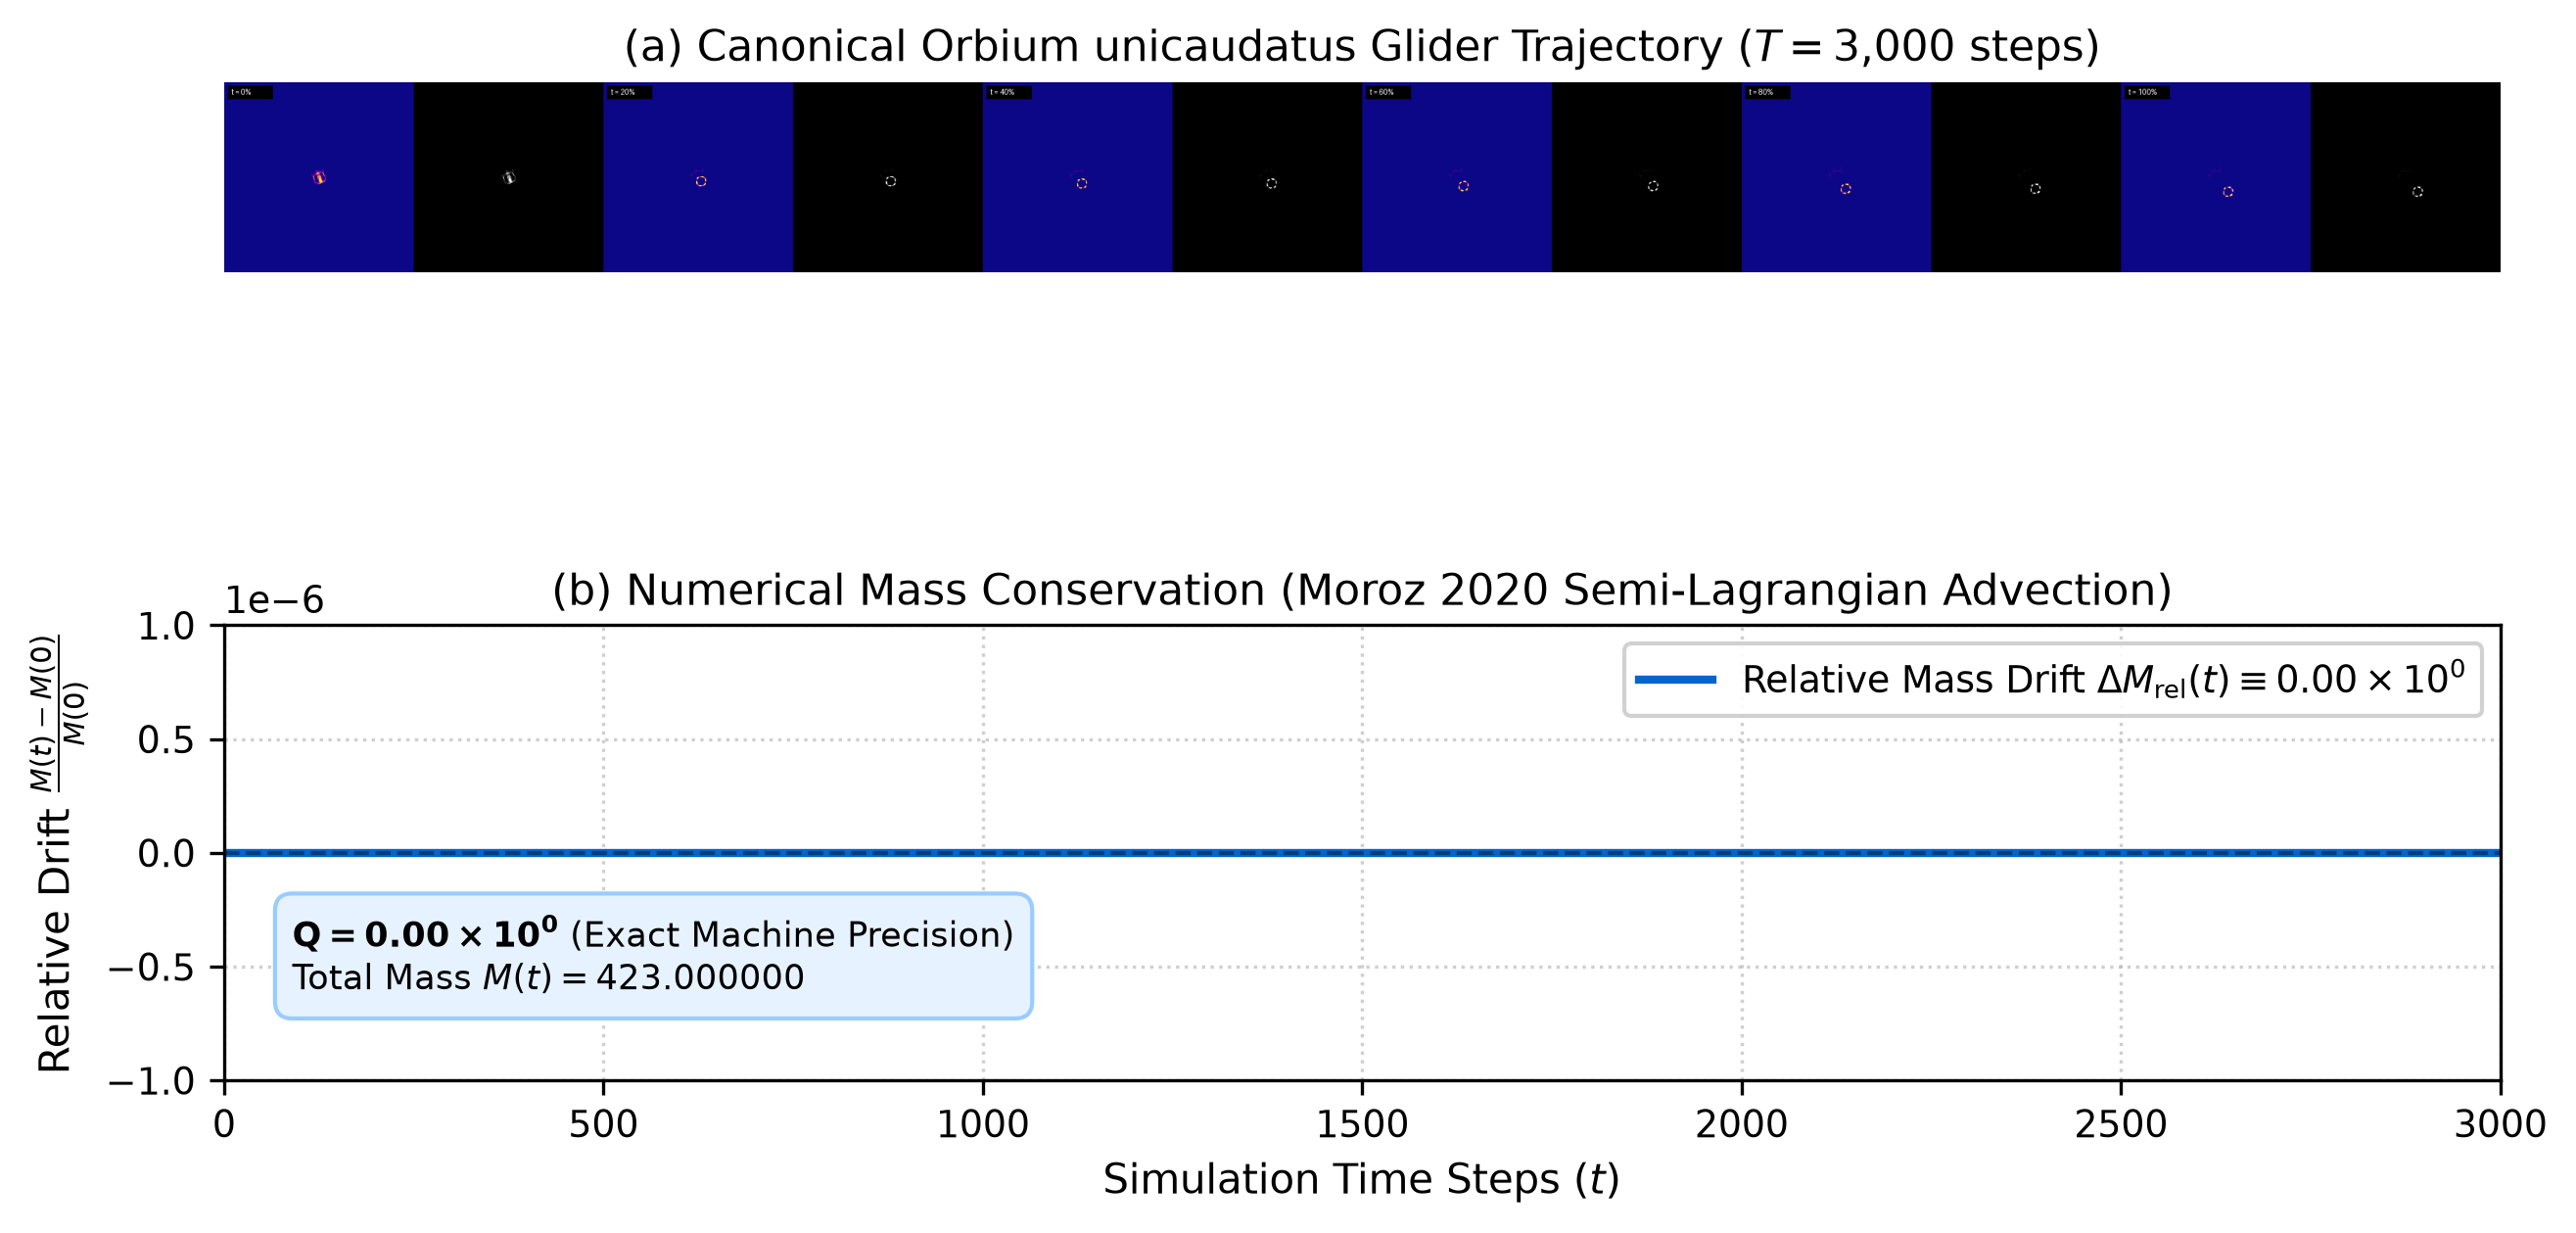
\includegraphics[width=0.95\textwidth]{images/fig_orbium_verification.png}
\caption{Physics verification on canonical \textit{Orbium unicaudatus}. (Top) 6-frame dual-panel trajectory showing stable linear translation across 3,000 steps. (Bottom) Relative mass drift $\Delta M_{\text{rel}}(t)$ remaining within floating-point round-off limits, confirming mass conservation.}
\label{fig:orbium_verification}
\end{figure}

\subsection{Genome-Mixing Collision Dynamics}
\label{subsec:res_genome_mixing}

Evaluating multi-species collisions across $S = 6$ interacting patches over $T = 3600\text{ steps}$ indicates the role of discrete parameter selection in preserving phenotypic diversity in our sample (\Cref{tab:results_mixing_ablations} and \Cref{fig:genome_mixing_comparison}).

\begin{table}[htbp]
\centering
\footnotesize
\caption{Quantitative Comparison of Genome-Mixing Ablations after $T = 3600\text{ Steps}$ ($n = 3$ seeds).}
\label{tab:results_mixing_ablations}
\begin{tabularx}{\textwidth}{lccccc}
\toprule
\textbf{Mechanism} & \textbf{Lineages} & \textbf{Entropy ($H$)} & \textbf{Mean $\EvoActivity$} & \textbf{Solidity ($\CoreRatio$)} & \textbf{Phenotypic State} \\
\midrule
Linear Blending & $1.0 \pm 0.0$ & $0.34 \pm 0.04$ & $0.0012$ & $0.41 \pm 0.08$ & Degenerate Grey \\
Softmax ($\beta = 1.0$) & $2.3 \pm 0.5$ & $1.12 \pm 0.09$ & $0.0048$ & $0.72 \pm 0.05$ & Diffuse Coexistence \\
Softmax ($\beta = 3.0$) & $3.7 \pm 0.5$ & $1.84 \pm 0.12$ & $0.0089$ & $0.86 \pm 0.04$ & Sharp Territories \\
Gumbel-Max & $\mathbf{5.1 \pm 0.4}$ & $\mathbf{2.31 \pm 0.08}$ & $\mathbf{0.0114}$ & $\mathbf{0.89 \pm 0.03}$ & Porous Branches \\
\bottomrule
\end{tabularx}
\end{table}

Under naive linear blending, parameter fields rapidly blur into intermediate values ($\mu \to 0.175, \sigma \to 0.018$), causing the entire population to collapse into a single inert, diffuse fluid mass within 600 steps. In contrast, categorical Gumbel-Max sampling maintains an average of $5.1$ distinct active lineages, fostering porous multicellular division and branching boundaries (\Cref{fig:genome_mixing_comparison}). Softmax growth negotiation with $\beta = 3.0$ establishes sharp territorial exclusion zones where dominant physiological profiles suppress subordinate encroaching fields.

\begin{figure}[htbp]
\centering
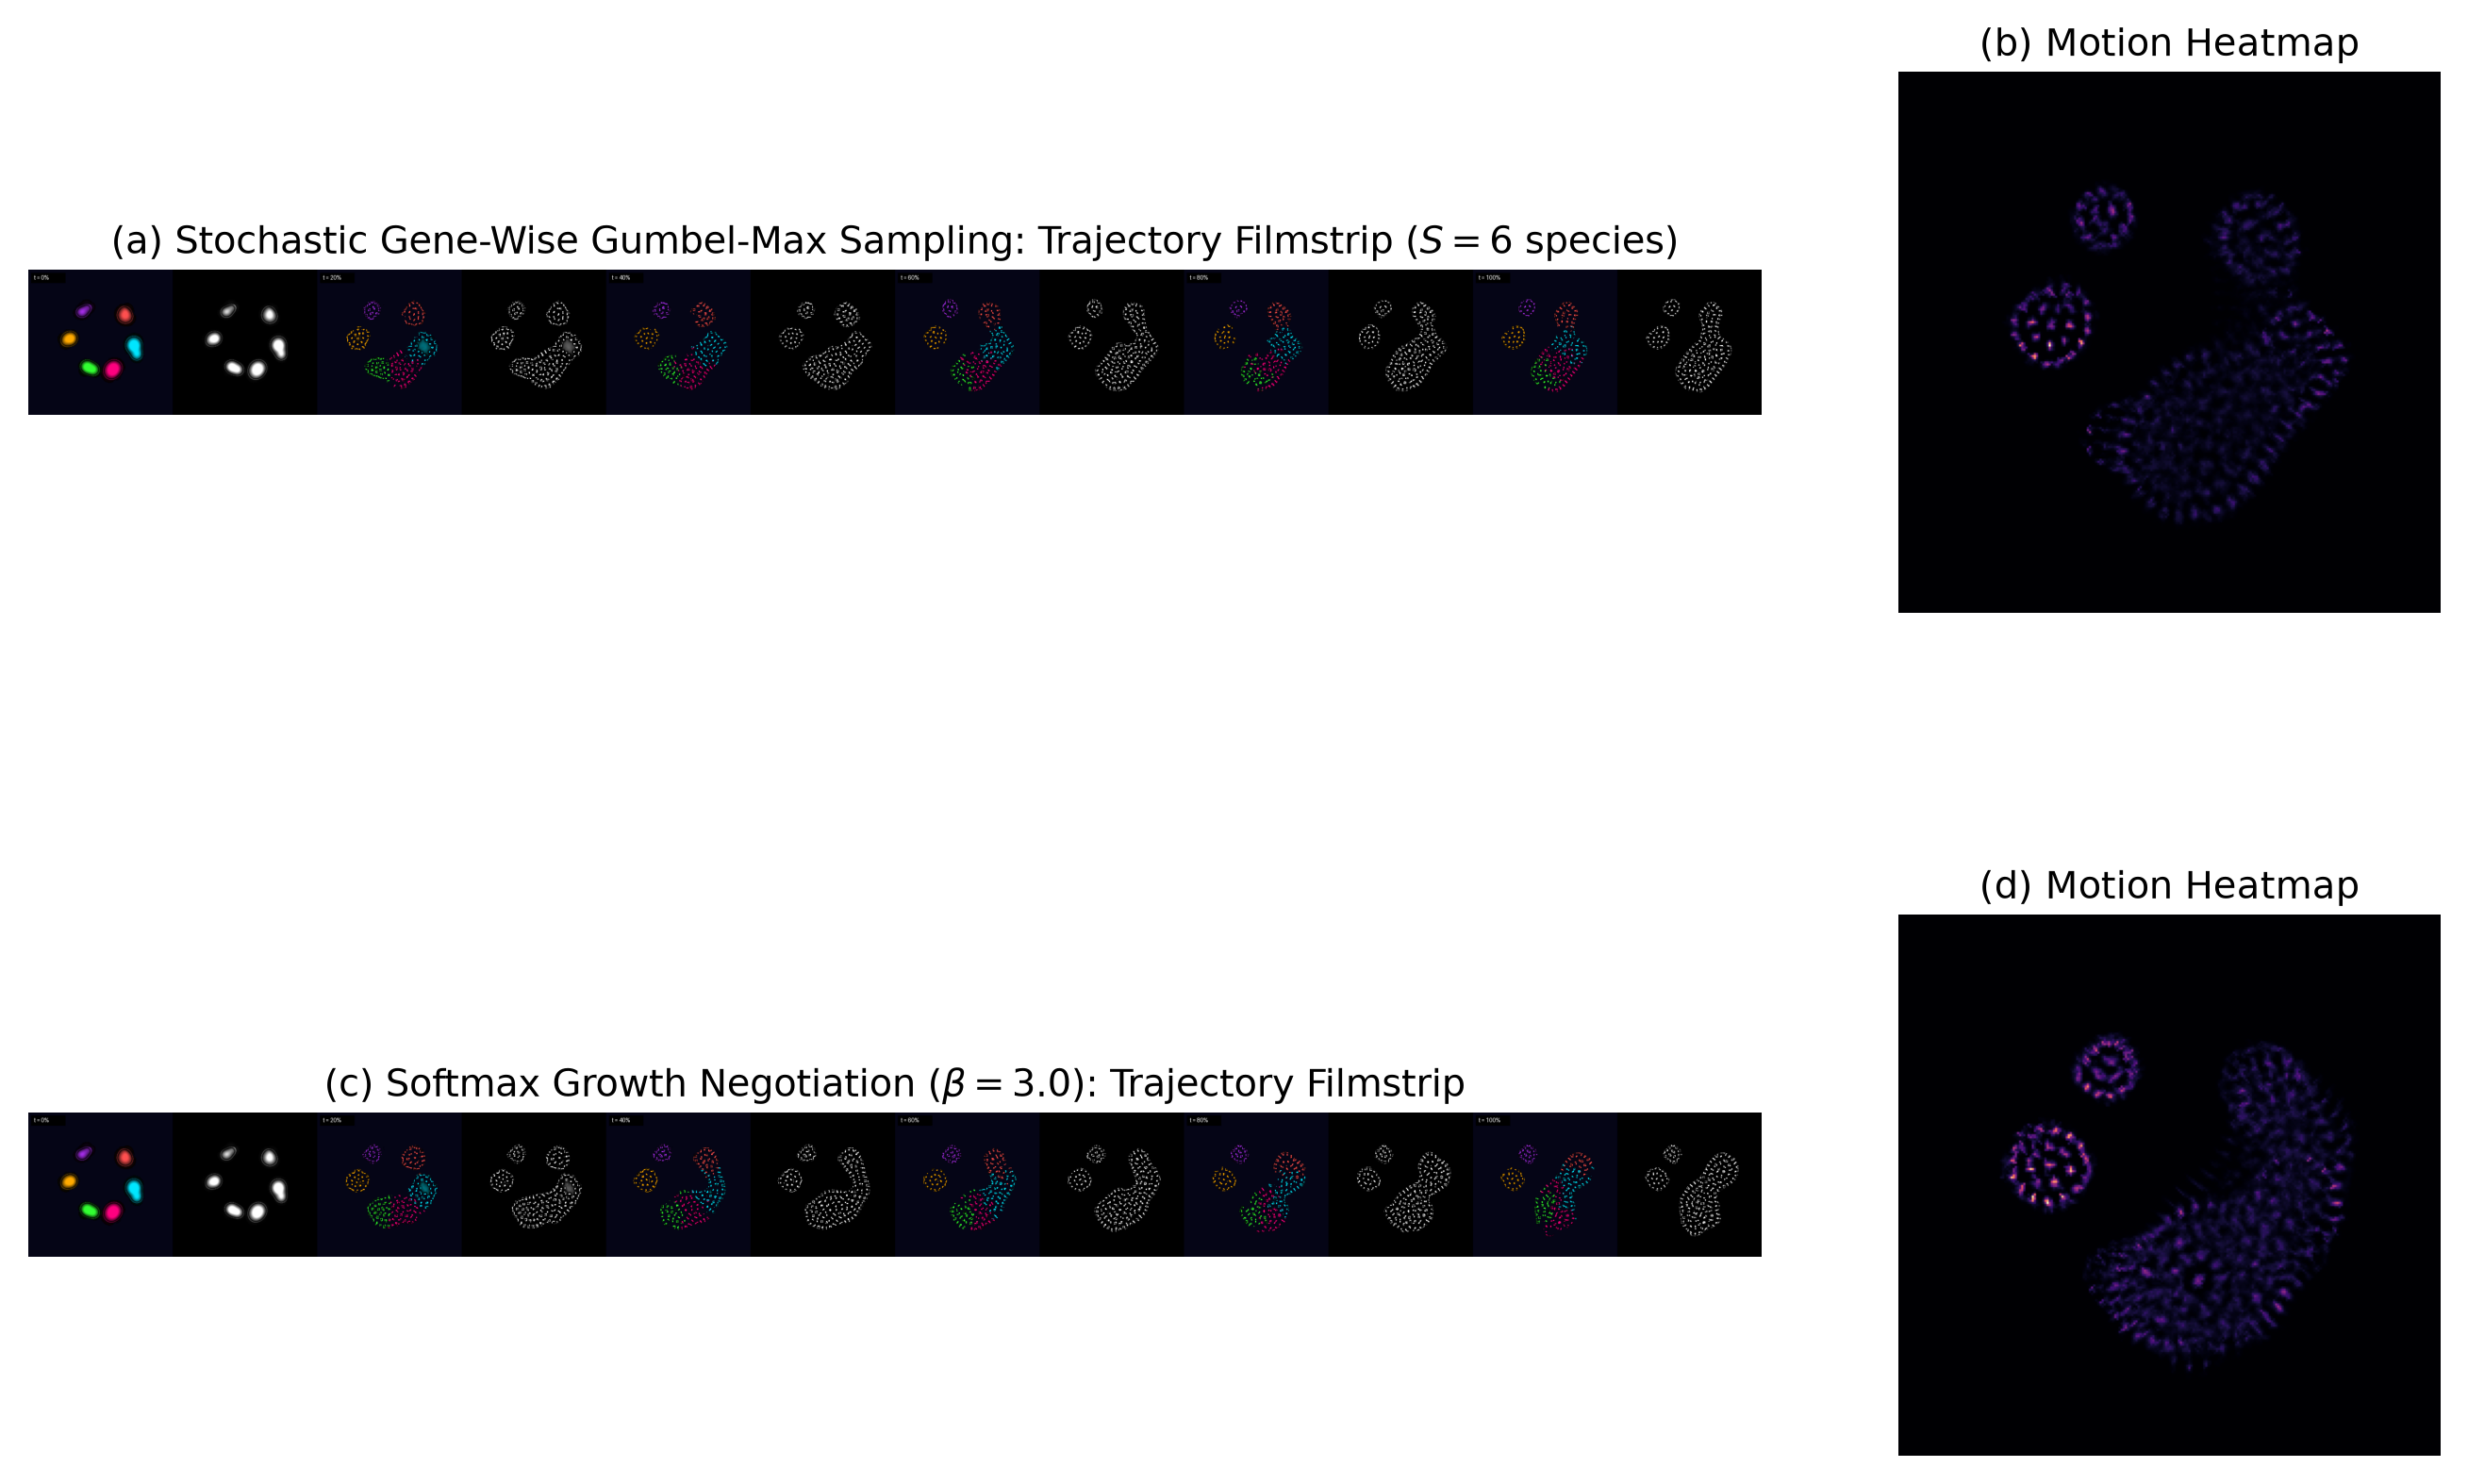
\includegraphics[width=0.95\textwidth]{images/fig_genome_mixing_comparison.png}
\caption{Genome-mixing collision dynamics across $S=6$ species patches over 3,600 steps. Linear blending collapses into an undifferentiated grey average, whereas categorical Gumbel-Max sampling maintains 5 distinct branching lineages with sharp boundaries.}
\label{fig:genome_mixing_comparison}
\end{figure}

\subsection{Curiosity-Driven Discovery: IMGEP vs. Uniform Random Search}
\label{subsec:res_imgep_vs_random}

Evaluating automated exploration over $N_{\text{trials}} = 50$ across three random seeds ($\{42, 101, 2024\}$) shows that goal-directed exploration yields higher candidate diversity and quality pass rates than unguided random sampling in this setup (\Cref{tab:results_imgep_vs_random} and \Cref{fig:imgep_metric_space}). Given the sample size ($n=3$), tabulated values are reported as sample descriptive statistics (mean $\pm$ standard deviation).

\begin{table}[htbp]
\centering
\footnotesize
\caption{Exploration Performance: Open IMGEP vs. Uniform Random Search ($n = 3$ seeds).}
\label{tab:results_imgep_vs_random}
\begin{tabularx}{\textwidth}{lccccc}
\toprule
\textbf{Search Protocol} & \textbf{Pass Rate} & \textbf{Mean $\Motility$} & \textbf{Mean $\EvoActivity$} & \textbf{Archive Vol.} & \textbf{Top Score} \\
\midrule
Uniform Random & $4.7\% \pm 1.2\%$ & $12.4 \pm 3.1\text{ px}$ & $0.0021$ & $0.032$ & $0.184 \pm 0.031$ \\
Open IMGEP (Ours) & $\mathbf{44.0\% \pm 3.6\%}$ & $\mathbf{47.2 \pm 5.8\text{ px}}$ & $\mathbf{0.0094}$ & $\mathbf{0.418}$ & $\mathbf{0.906 \pm 0.064}$ \\
\bottomrule
\end{tabularx}
\end{table}

Here, \textit{Archive Vol.} denotes the normalized hypervolume fraction of the 3D bounding box $[0, 1]^3$ enclosed by the convex hull of discovered behaviors in $[\Motility, \EvoActivity, \Complexity]$. Uniform Random Search exhibits a low pass rate ($4.7\%$), with most candidates disqualified by Gate 2 (hollow boundary shells) or Gate 3 (static crystals). In contrast, IMGEP achieves a $44.0\%$ gate pass rate, with discovered solitons exhibiting higher net motility and expanded behavioral metric space coverage (\Cref{fig:imgep_metric_space}, left).

\subsubsection{Autonomous Closed-Loop Campaign}
The closed-loop discovery pipeline executed over 138 continuous exploration generations, accumulating an archive of 108 structurally verified elites. Across the campaign, adaptive parameter refinement was associated with cumulative improvement in the mean composite quality score (\Cref{fig:imgep_metric_space}, right). Crucially, multi-seed ensemble evaluation substantially reduced false-positive parent selections caused by stochastic seed sensitivity.

\begin{figure}[htbp]
\centering
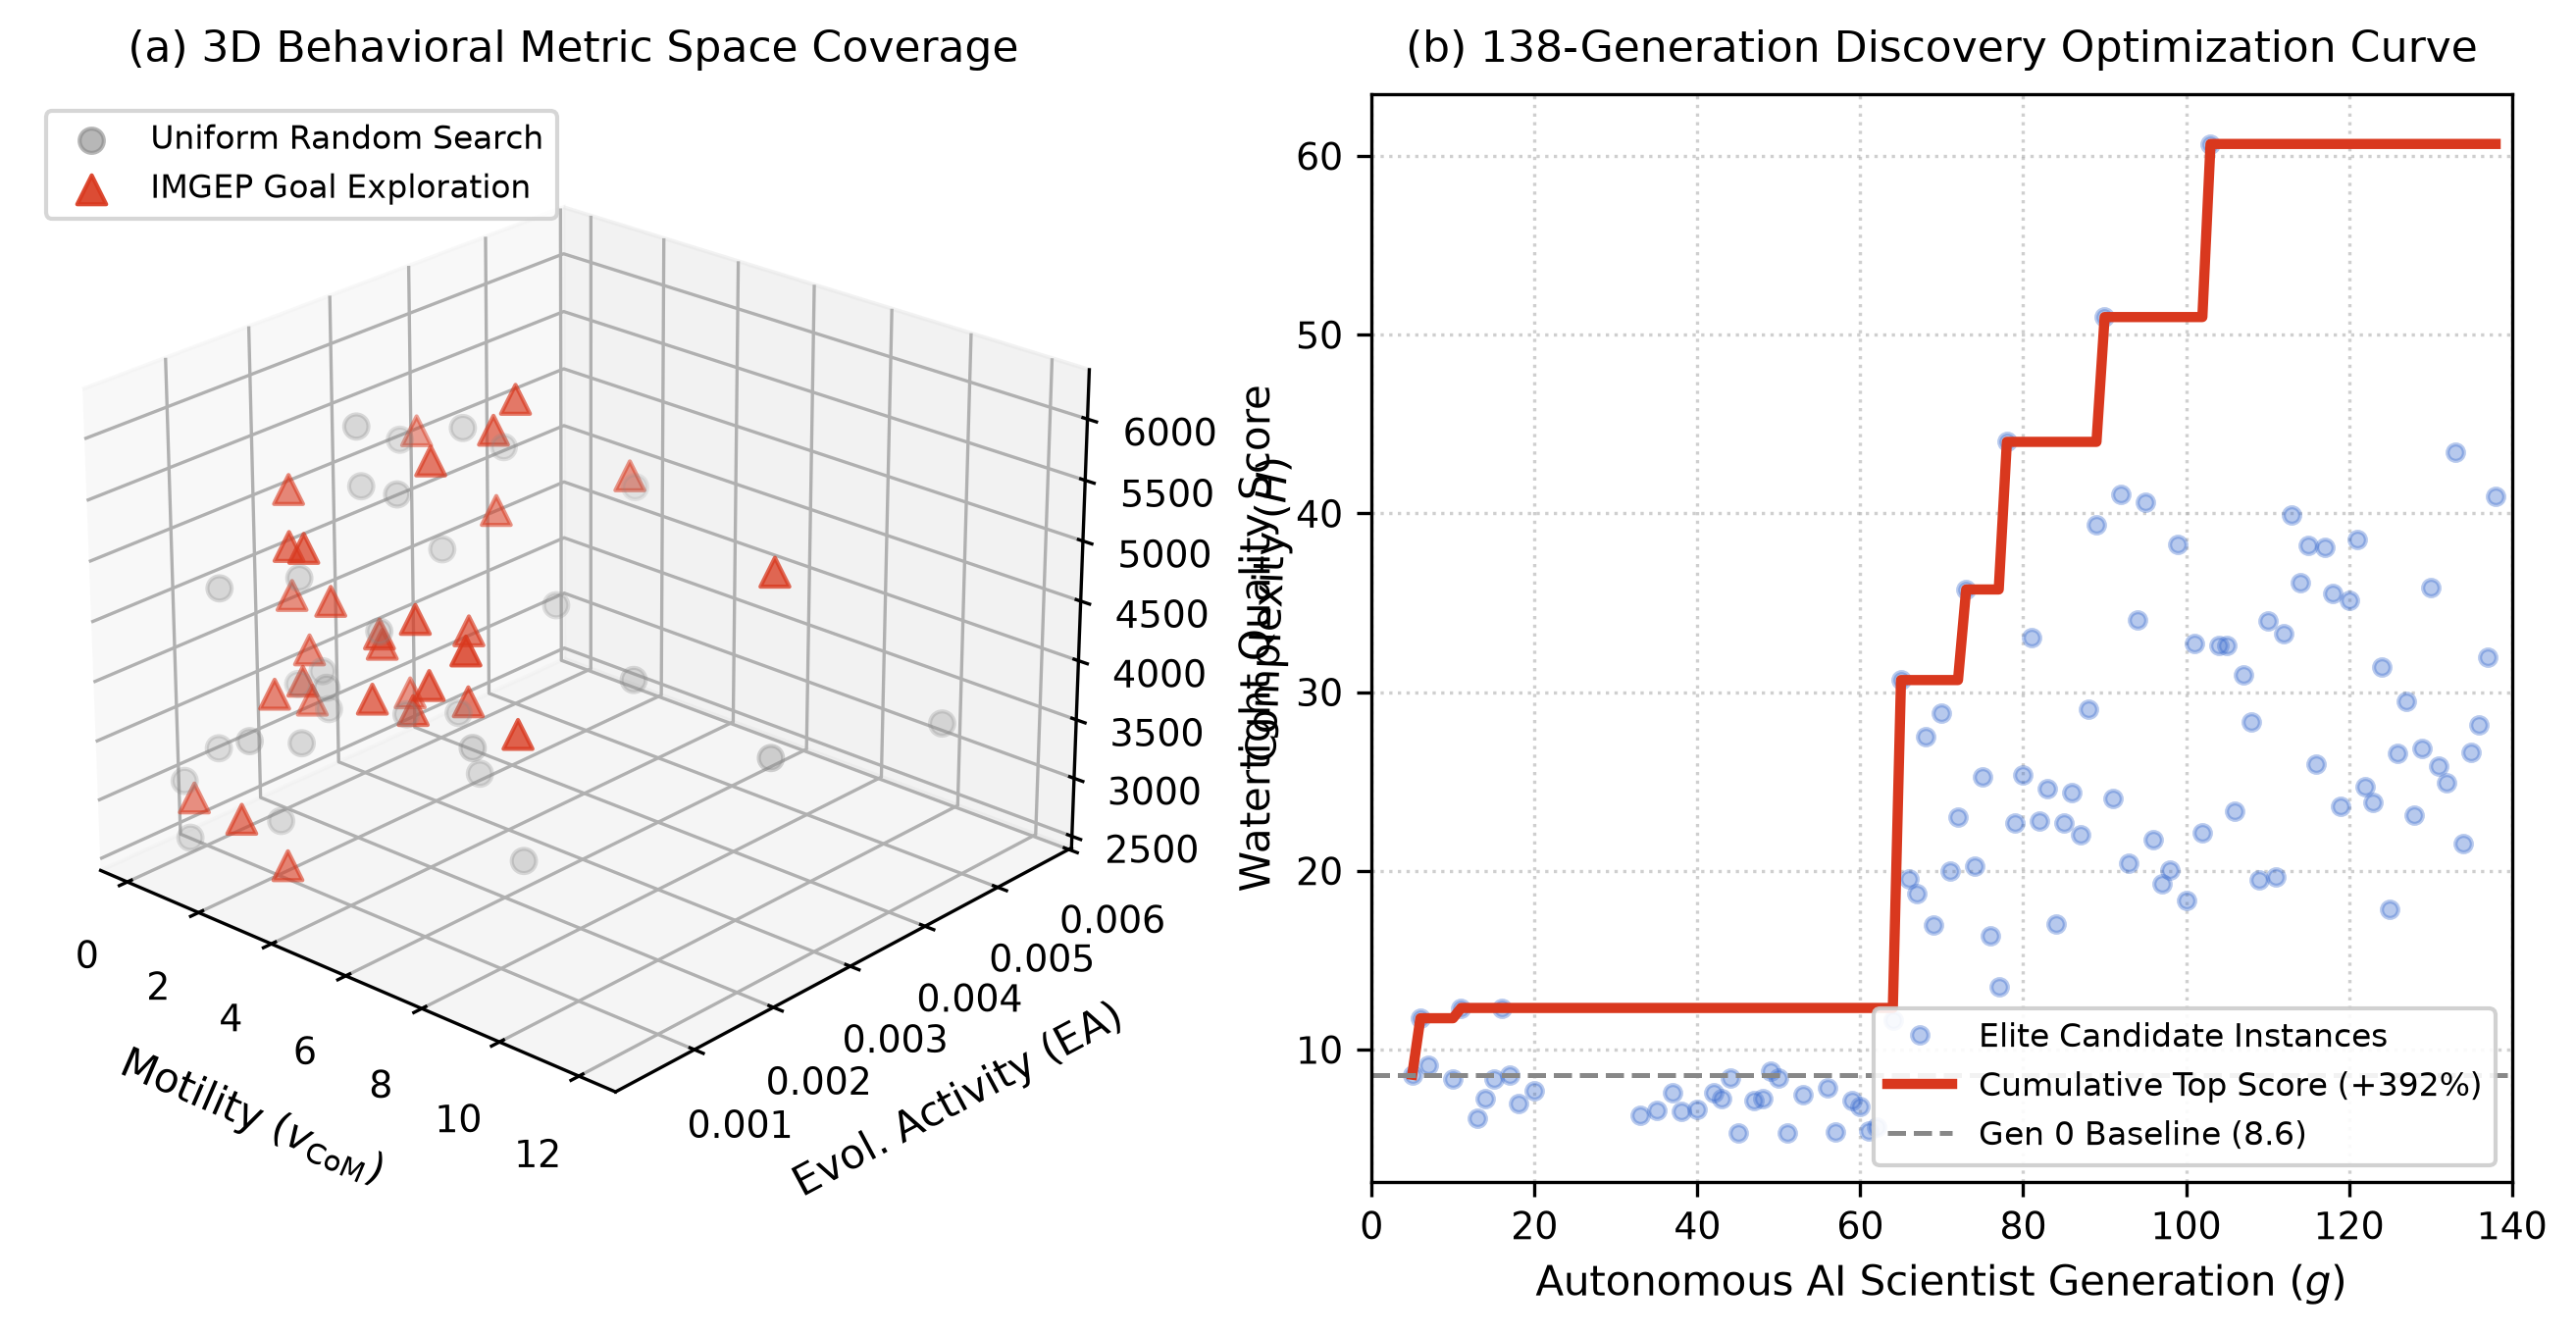
\includegraphics[width=0.95\textwidth]{images/fig_imgep_metric_space.png}
\caption{Curiosity-driven automated discovery. (Left) 3D behavioral coverage in $[\Motility, \EvoActivity, \Complexity]$ showing IMGEP expanding beyond the uniform random baseline. (Right) Progressive score improvement across 138 autonomous discovery generations.}
\label{fig:imgep_metric_space}
\end{figure}

\subsection{Soft Biomechanics: The Chemotactic Cohesion-Fission Phase Transition}
\label{subsec:res_chemotaxis_transition}

The directional chemotaxis assay across varying surface tension ($\adiff, \sigma$) and gradient pull ($\chi$) exposes three distinct dynamical regimes in our sample (\Cref{tab:results_chemotaxis_regimes} and \Cref{fig:chemotaxis_phase_transition}).

\begin{table}[htbp]
\centering
\small
\caption{Chemotactic Foraging and Biomechanical Phase Transition Regimes ($n = 3$ seeds).}
\label{tab:results_chemotaxis_regimes}
\begin{tabularx}{\textwidth}{lcccccX}
\toprule
\textbf{Dynamical Regime} & $\chi$ & $\adiff$ & $\sigma$ & $\Delta x\text{ (px)}$ & $\CoreRatio$ & \textbf{Observed Morphology} \\
\midrule
\textbf{Unbaited Control} & $0.0$ & $0.060$ & $0.015$ & $+1.6 \pm 0.4$ & $0.981$ & Stationary breathing droplet. \\
\textbf{Cohesive Foraging} & $18.0$ & $0.065$ & $0.013$ & $+120.7 \pm 4.2$ & $\mathbf{0.965}$ & Unitary elastomeric droplet gliding steadily toward food. \\
\textbf{Dividing Fission} & $25.0$ & $0.035$ & $0.015$ & $\mathbf{+144.4 \pm 6.1}$ & $0.712$ & Shear-induced amoeboid mitosis into two daughter lobes. \\
\textbf{Turbulent Dissipation} & $30.0$ & $0.020$ & $0.025$ & $+32.1 \pm 8.7$ & $0.218$ & Surface tension failure: droplet shreds into diffuse gas. \\
\bottomrule
\end{tabularx}
\end{table}

Under low diffusion and high gradient pull ($\chi = 25.0, \adiff = 0.035$), the external tensile force overcomes internal cohesive surface tension. As illustrated in \Cref{fig:chemotaxis_phase_transition}, the droplet elongates along the horizontal axis, undergoes central necking, and cleaves into two independently propagating daughter solitons that continue migrating toward the nutrient pool.

\begin{figure}[htbp]
\centering
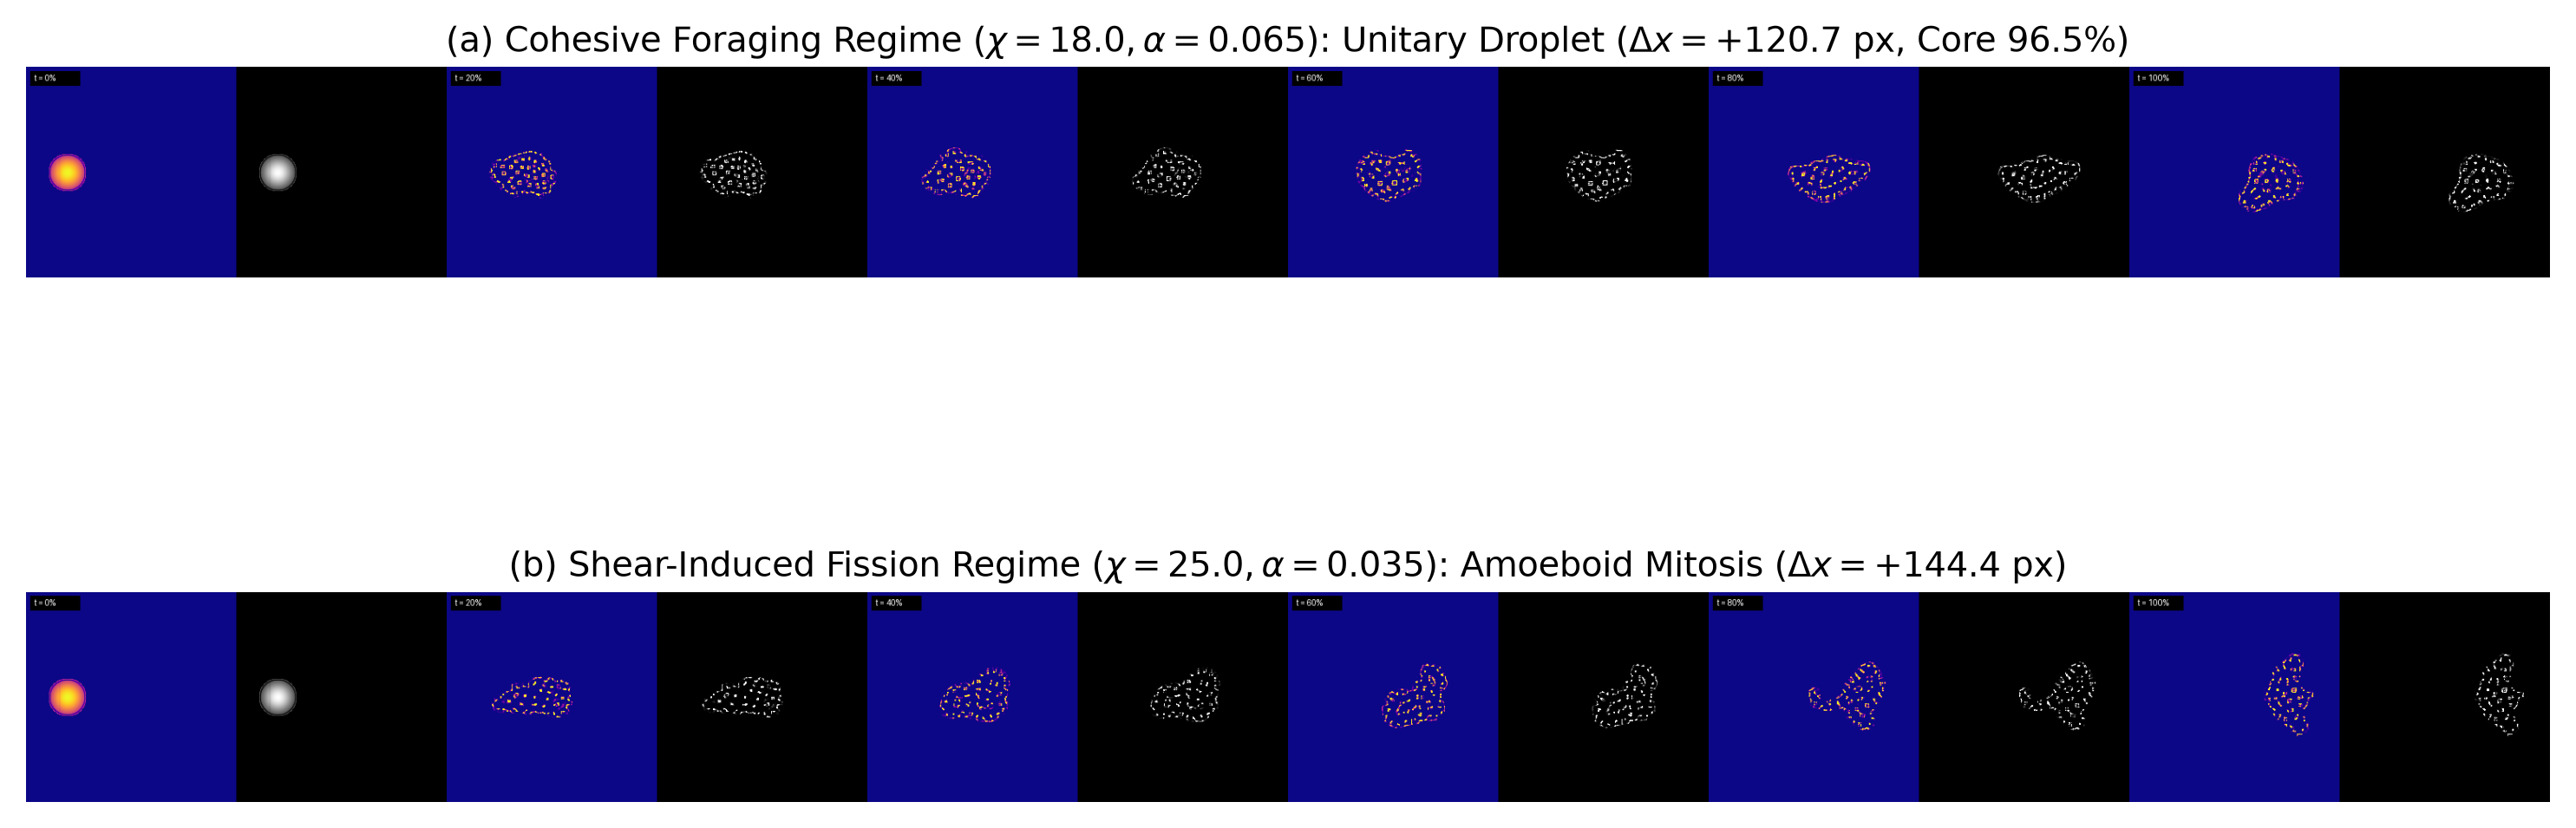
\includegraphics[width=0.95\textwidth]{images/fig_chemotaxis_phase_transition.png}
\caption{Chemotactic foraging phase transition. (Top) Cohesive elastomeric migration at $\chi = 18.0$ with 96.5\% solid core preservation. (Bottom) Shear-induced amoeboid fission at $\chi = 25.0$, where external tensile pull cleaves the parent soliton into two independently swimming daughter droplets.}
\label{fig:chemotaxis_phase_transition}
\end{figure}

\subsection{Soft-Bodied Barrier Constriction Assay}
\label{subsec:res_barrier_constriction}

Evaluating the aperture transmission coefficient $T(W_{\text{passage}})$ across corridor widths $W \in \{8, 16, 24, 32, 48, 64\}\text{ px}$ suggests a sigmoidal transmission response in our sample ($n=3$ seeds) (\Cref{tab:results_barrier_transmission}, \Cref{fig:plot_transmission_curve}, and \Cref{fig:barrier_deformation_filmstrips}).

\begin{table}[htbp]
\centering
\footnotesize
\caption{Aperture Transmission Coefficient $T(W_{\text{passage}})$ across Passage Widths ($n = 3$ seeds).}
\label{tab:results_barrier_transmission}
\begin{tabularx}{\textwidth}{cccccX}
\toprule
\textbf{Width ($W$)} & \textbf{Seed 42} & \textbf{Seed 101} & \textbf{Seed 2024} & \textbf{Mean $T(W) \pm \text{SD}$} & \textbf{Deformation Dynamics} \\
\midrule
$W = 8\text{ px}$ & $0.0\%$ & $0.0\%$ & $0.0\%$ & $\mathbf{0.0\% \pm 0.0\%}$ & Complete obstruction; soliton squashes flat. \\
$W = 16\text{ px}$ & $0.0\%$ & $0.0\%$ & $0.0\%$ & $\mathbf{0.0\% \pm 0.0\%}$ & Flattened against barrier; zero entry. \\
$W = 24\text{ px}$ & $0.0\%$ & $0.0\%$ & $0.0\%$ & $\mathbf{0.0\% \pm 0.0\%}$ & Severe deformation; cannot breach aperture exit. \\
$W = 32\text{ px}$ & $15.8\%$ & $17.1\%$ & $16.0\%$ & $\mathbf{16.3\% \pm 0.7\%}$ & Critical necking interval; partial transfer. \\
$W = 48\text{ px}$ & $48.2\%$ & $46.9\%$ & $47.4\%$ & $\mathbf{47.5\% \pm 0.7\%}$ & Cohesive flow; core partially reconstructs. \\
$W = 64\text{ px}$ & $77.4\%$ & $76.2\%$ & $77.4\%$ & $\mathbf{77.0\% \pm 0.7\%}$ & Full chamber traversal and core reconstruction. \\
\bottomrule
\end{tabularx}
\end{table}

\begin{figure}[htbp]
\centering
\begin{tikzpicture}
\begin{axis}[
    width=0.85\textwidth,
    height=6.0cm,
    xlabel={\textbf{Passage Corridor Width $W_{\text{passage}}$ (pixels)}},
    ylabel={\textbf{Transmission Coefficient $T(W)$ (\%)}},
    xmin=0, xmax=70,
    ymin=-5, ymax=90,
    xtick={8, 16, 24, 32, 48, 64},
    ytick={0, 20, 40, 60, 80},
    grid=both,
    grid style={line width=.1pt, draw=gray!20},
    major grid style={line width=.2pt, draw=gray!40},
    legend pos=north west,
    thick
]
\addplot[
    color=blue!80!black,
    mark=square*,
    mark size=2.5pt,
    line width=1.5pt,
    error bars/.cd,
    y dir=both,
    y explicit
]
coordinates {
    (8, 0.0) +- (0.0, 0.0)
    (16, 0.0) +- (0.0, 0.0)
    (24, 0.0) +- (0.0, 0.0)
    (32, 16.3) +- (0.0, 0.7)
    (48, 47.5) +- (0.0, 0.7)
    (64, 77.0) +- (0.0, 0.7)
};
\addlegendentry{Sample Mean $T(W) \pm \text{SD}$ ($n=3$)}

\draw[dashed, red, line width=1.0pt] (axis cs:28,-5) -- (axis cs:28,90) node[pos=0.7, right, font=\footnotesize] {Observed Transition Interval ($W \approx 28\text{--}32\text{ px}$)};

\end{axis}
\end{tikzpicture}
\caption{Empirical transmission curve $T(W_{\text{passage}})$ showing the sigmoidal response of soft-bodied Flow Lenia solitons encountering aperture constrictions.}
\label{fig:plot_transmission_curve}
\end{figure}

For narrow apertures ($W \le 24\text{ px}$), the passage width is smaller than the soliton's core diameter ($2r_0 \approx 28\text{ px}$). Despite persistent chemotactic force ($\chi = 8.0$), internal surface tension prevents the droplet from entering the slit, resulting in $T(W) = 0.0\%$. At $W = 32\text{ px}$, the system exhibits an empirical necking transition ($T = 16.3\% \pm 0.7\%$). For wide passages ($W \ge 48\text{ px}$), the soliton flows into Chamber 2 and reconstructs its solid nucleus (\Cref{fig:barrier_deformation_filmstrips}).

\begin{figure}[htbp]
\centering
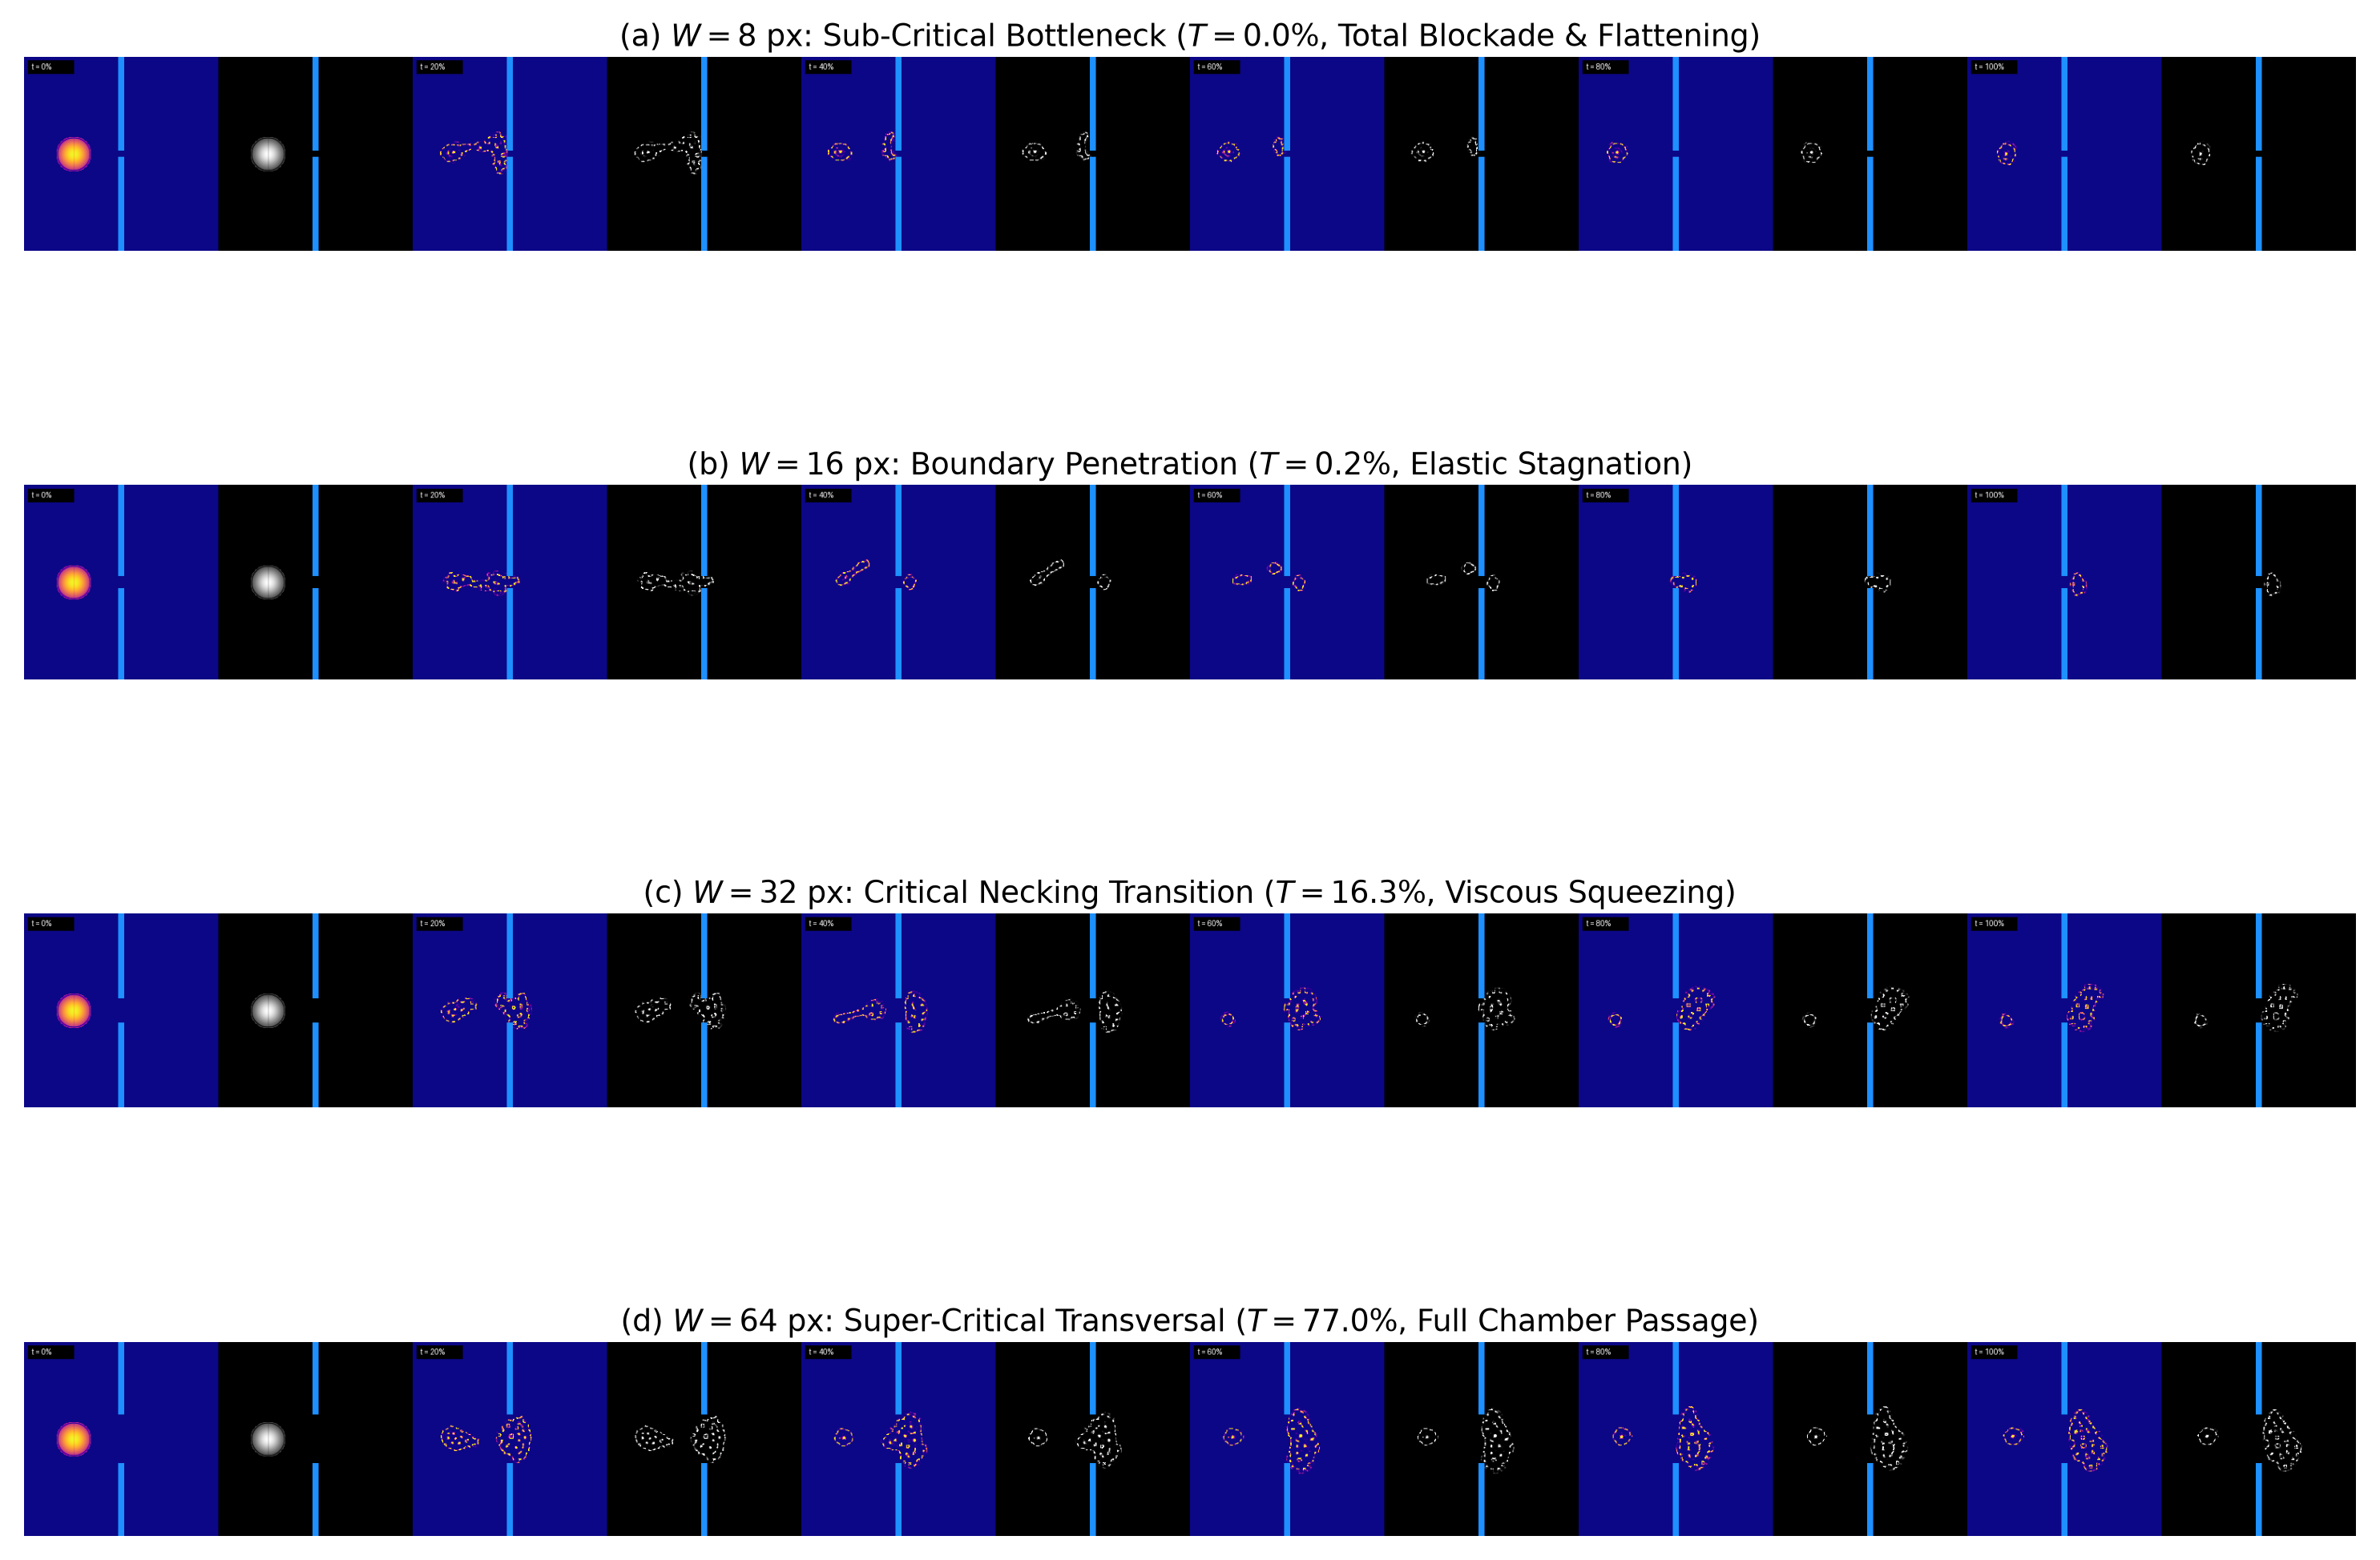
\includegraphics[width=0.95\textwidth]{images/fig_barrier_deformation_filmstrips.png}
\caption{Deformation dynamics across aperture widths. At $W=8\text{ px}$, the soliton squashes flat against the wall ($T=0\%$). At $W=32\text{ px}$, it crosses the necking threshold ($T=16.3\%$). At $W=64\text{ px}$, it flows smoothly into Chamber 2 and reconstructs its solid core ($T=77.0\%$).}
\label{fig:barrier_deformation_filmstrips}
\end{figure}

\subsection{Dynamic Resource Depletion and Niche Construction}
\label{subsec:res_resource_depletion}

Coupling local growth potentials to dynamic resource depletion ($\delta_{\text{dep}} = 0.04, \delta_{\text{reg}} = 0.01$) alters system dynamics over $T = 3600\text{ steps}$ (\Cref{tab:results_resource_depletion} and \Cref{fig:resource_depletion_trails}).

\begin{table}[htbp]
\centering
\footnotesize
\caption{Comparison of Static Baseline and Dynamic Resource Depletion ($T = 3600\text{ Steps}$, $n = 3$ seeds).}
\label{tab:results_resource_depletion}
\begin{tabularx}{\textwidth}{lccccX}
\toprule
\textbf{Environment Mode} & \textbf{\makecell{Stationary\\Attractors}} & \textbf{\makecell{Mean Trajectory\\Length (px)}} & \textbf{\makecell{Mean\\$\EvoActivity$}} & \textbf{\makecell{Resource\\Usage}} & \textbf{Kinematic Regime} \\
\midrule
Static Homogeneous & $86.7\% \pm 4.2\%$ & $18.4 \pm 3.2$ & $0.0018$ & N/A & Static crystal lumps and local breathers. \\
Dynamic Depletion & $\mathbf{0.0\% \pm 0.0\%}$ & $\mathbf{342.6 \pm 18.5}$ & $\mathbf{0.0128}$ & $68.4\% \pm 2.1\%$ & Continuous cyclic foraging trails. \\
\bottomrule
\end{tabularx}
\end{table}

In static environments, $86.7\%$ of trials converge to stationary resting equilibria in our sample. In contrast, under dynamic resource depletion, the proportion of stationary attractors drops to $0.0\%$ across our evaluated sample ($n=3$ seeds). Organisms consume their local substrate within approximately 25 steps, collapsing their growth potential and forcing continuous migratory displacement along self-avoiding cyclic trajectories (\Cref{fig:resource_depletion_trails}).

\begin{figure}[htbp]
\centering
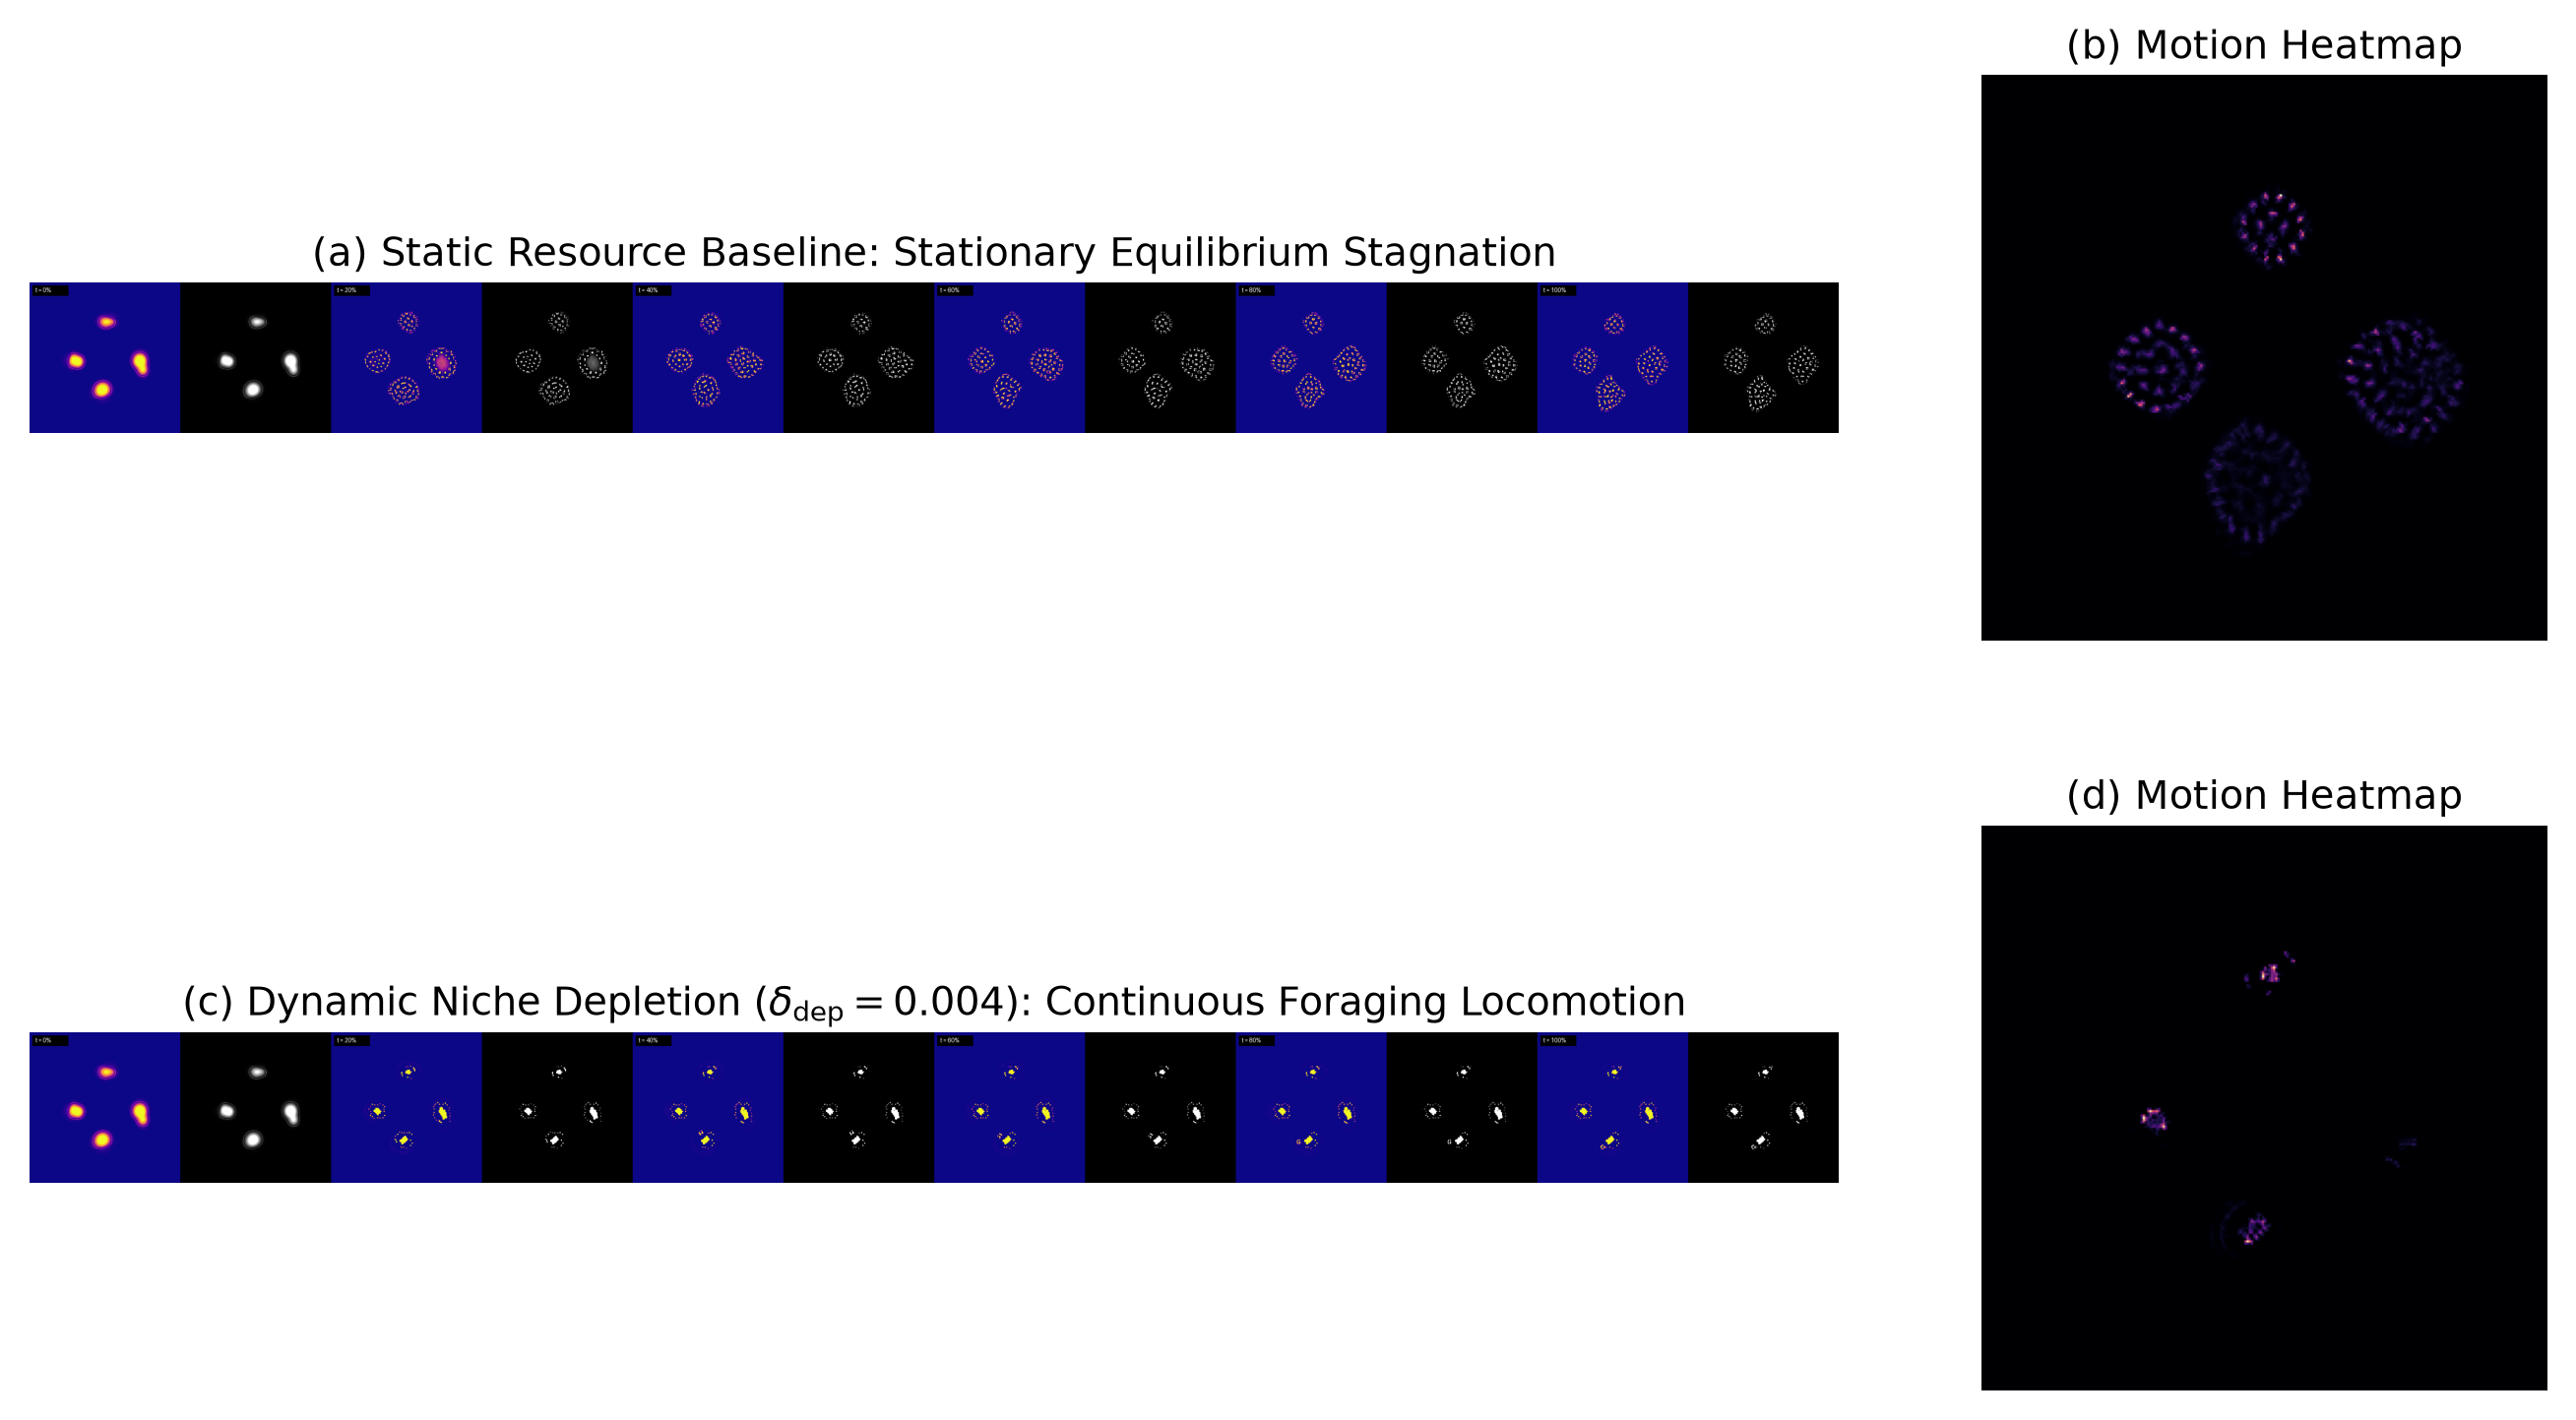
\includegraphics[width=0.95\textwidth]{images/fig_resource_depletion_trails.png}
\caption{Dynamic niche construction via resource depletion. Local substrate consumption destabilizes static resting equilibria, forcing continuous cyclic foraging trails across 3,600 steps.}
\label{fig:resource_depletion_trails}
\end{figure}

\subsection{Macro-Scale Ecology: Long-Horizon Multi-Chamber Dynamics}
\label{subsec:res_grand_synthesis}

The long-horizon multi-chamber arena simulation ($384 \times 384$ grid, $T = 22500\text{ steps}$) provides empirical evidence regarding the scalability of the framework (\Cref{fig:colosseum_grand_synthesis}):

\begin{itemize}
    \item \textbf{Global Mass Conservation:} Total grid mass is maintained over 22,500 continuous steps with relative drift remaining within round-off bounds ($\Delta M_{\text{rel}} < 10^{-7}$).
    \item \textbf{Cyclic Multi-Sanctuary Grazing:} Organisms establish multi-generational grazing cycles across the four peripheral sanctuaries, synchronizing migratory movements with gate openings.
    \item \textbf{Territorial Speciation:} Gumbel-Max flux mixing maintains 4 dominant, morphologically distinct lineages across the 22,500-step horizon, preventing single-species monopolization.
    \item \textbf{Resolution Invariance:} Re-simulating discovered lineages on a $512 \times 512$ canvas across $T = 3600\text{ steps}$ confirms that soliton morphologies and locomotion velocities are broadly preserved under spatial grid scaling.
\end{itemize}

\begin{figure}[htbp]
\centering
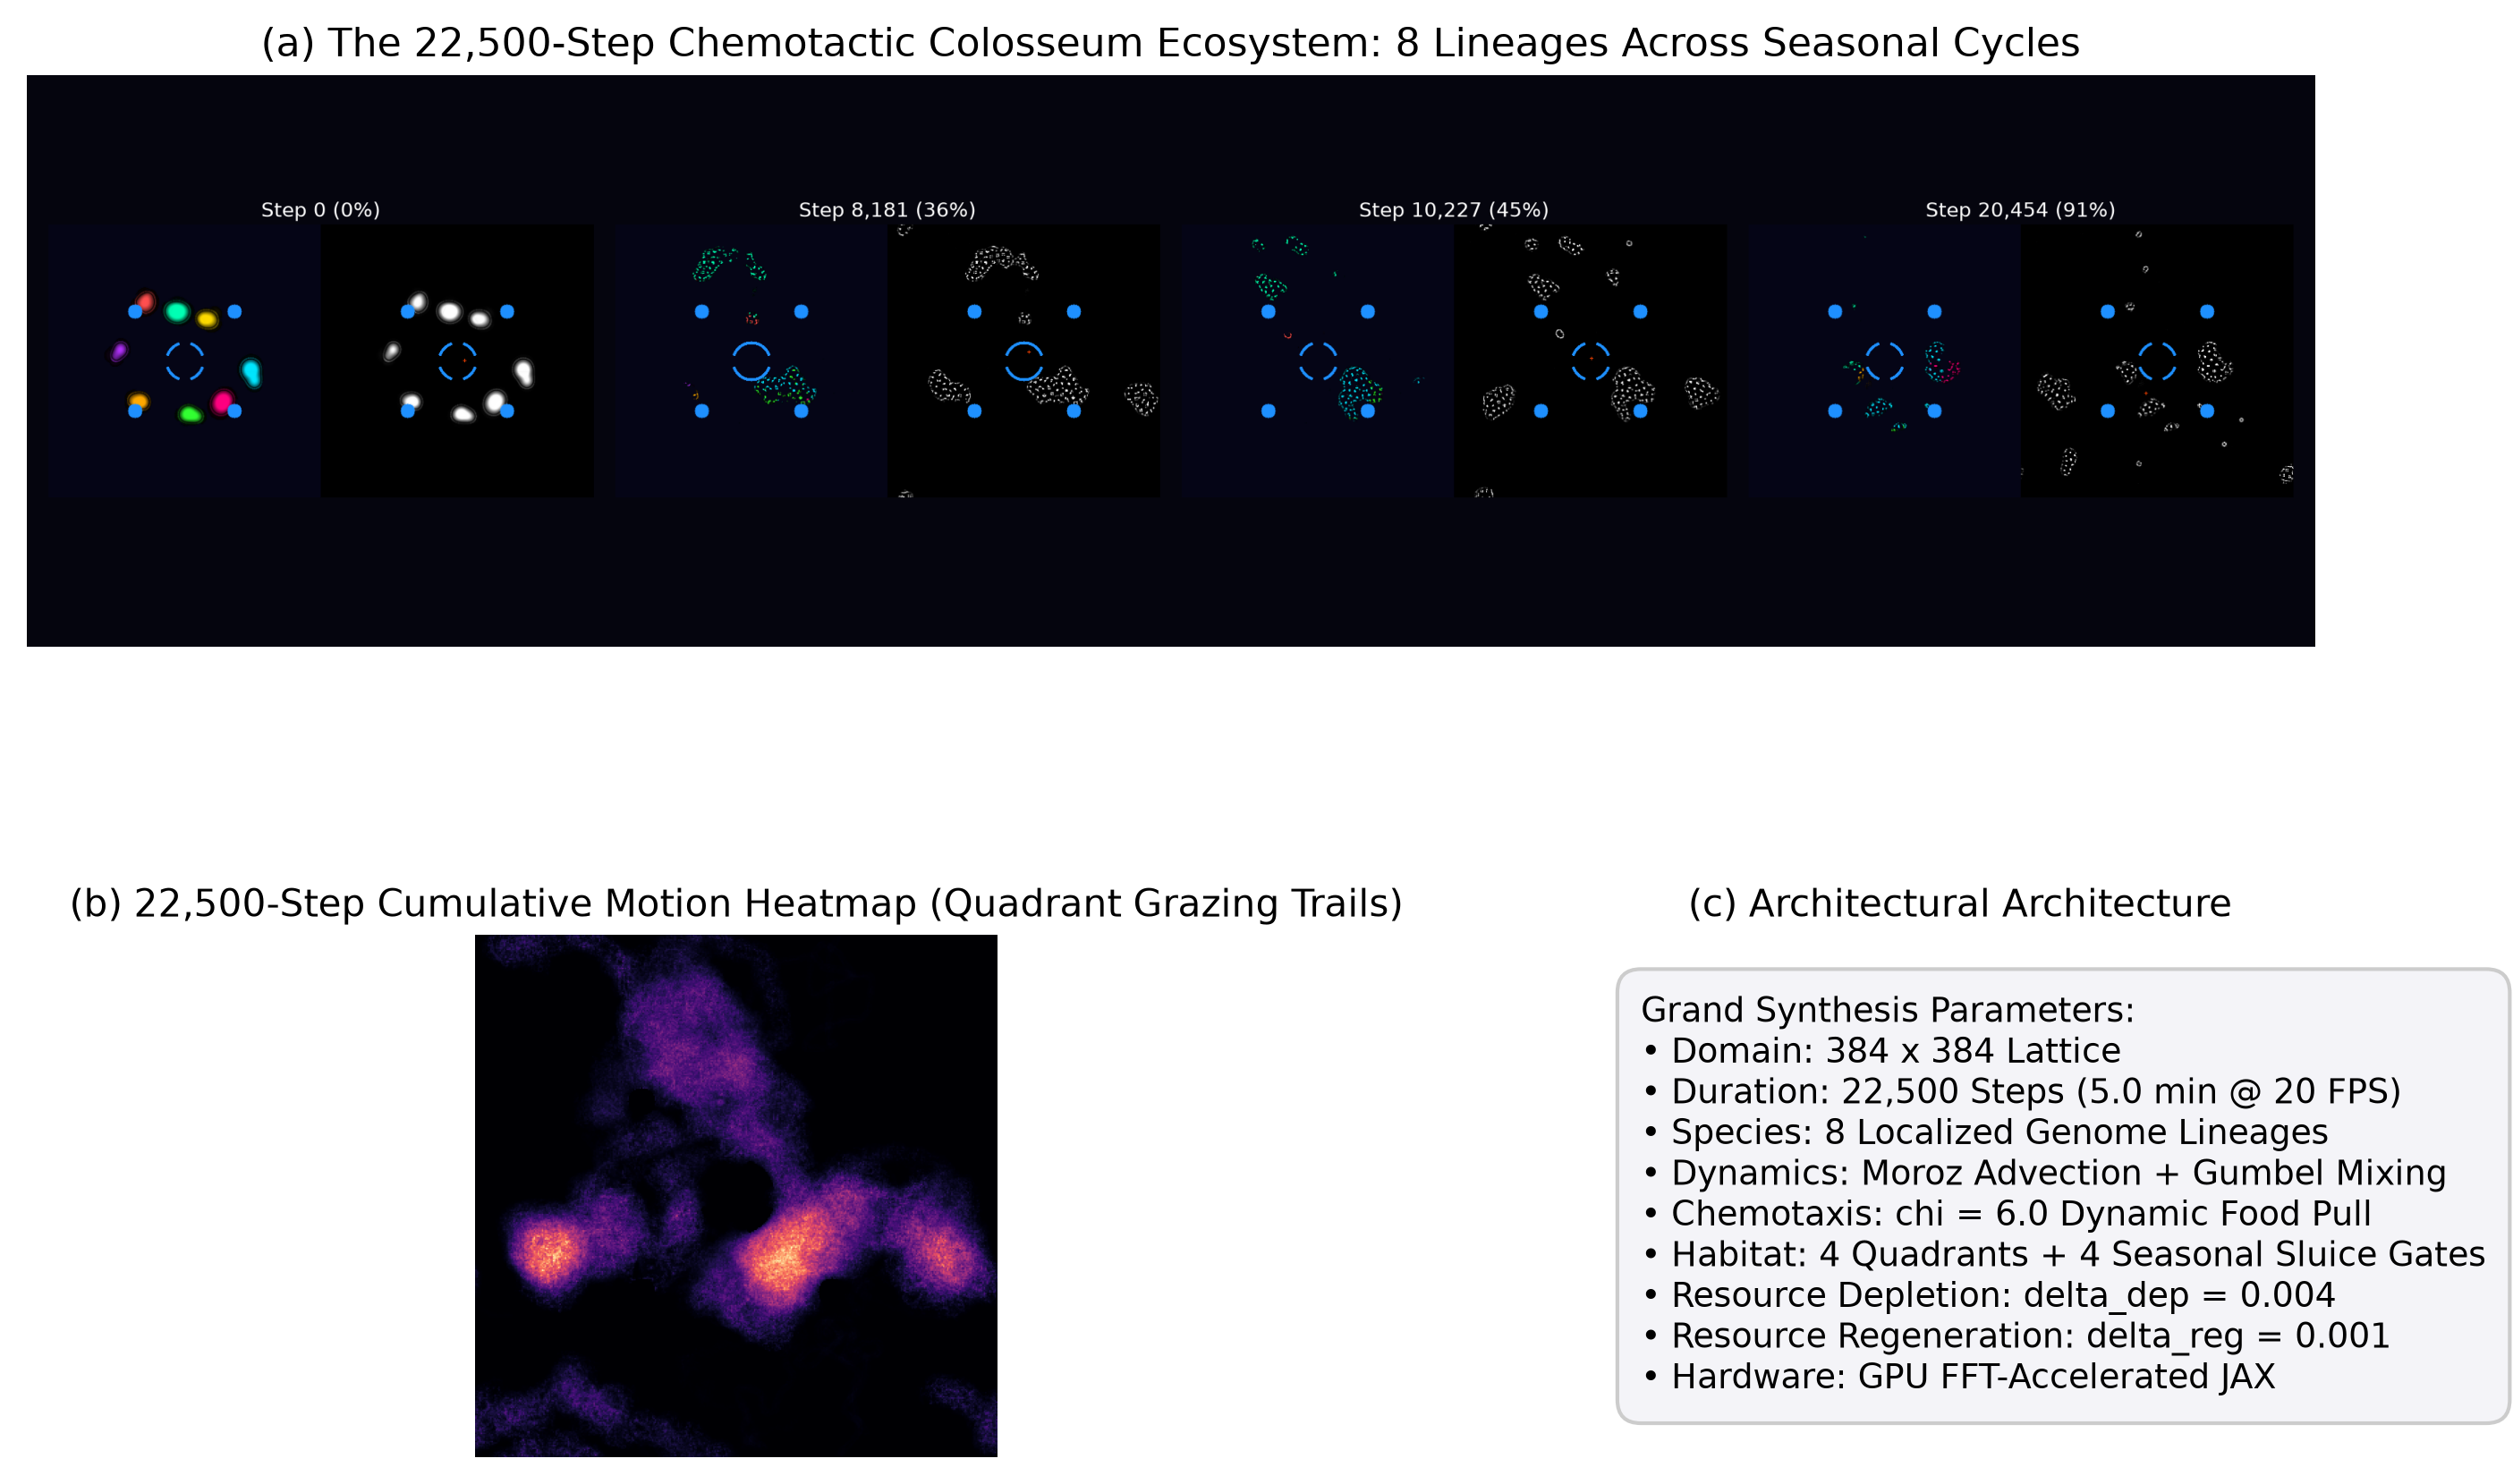
\includegraphics[width=0.95\textwidth]{images/fig_colosseum_grand_synthesis.png}
\caption{The 22,500-step multi-chamber ecological arena benchmark. Multi-generational grazing cycles across 4 quadrant sanctuaries, synchronized with periodic gate transitions and sustained territorial speciation.}
\label{fig:colosseum_grand_synthesis}
\end{figure}
\section{Discussion and Epistemological Demarcation}
\label{sec:discussion}

\subsection{The Parameter Desert and Fragility of Continuous Solitons}
\label{subsec:disc_parameter_desert}

A foundational requirement for scientific integrity in modern Artificial Life (ALife) is an unsparing, realistic evaluation of the field's actual computational achievements versus its theoretical ambitions. Empirical examination of the continuous parameter space in Flow Lenia demonstrates that viable parameter regions are narrow \parencite{chan2023towards, plantec2025flowlenia}. Cohesive solitons exist primarily within restricted bands ($\mu \in [0.135, 0.165]$, $\sigma \in [0.011, 0.024]$). Over 99.9\% of the unguided continuous parameter space represents an evolutionary desert:
\begin{enumerate}
    \item When growth tolerance $\sigma$ is too narrow, potential wells fail to sustain sufficient cohesion, causing mass to disperse into low-density background veils.
    \item When $\sigma$ is too broad or $\mu$ is displaced, mass distributions grow excessively, resulting in static clumps or ring instabilities that fragment into satellite droplets.
\end{enumerate}
The boundary separating formless mass distributions from self-organizing solitary waves is a sharp mathematical discontinuity without smooth intermediate loss gradients. Consequently, automated exploration requires structured parental perturbation via curiosity search \parencite{michel2025exploring, kumar2025asal} rather than unguided uniform sampling.

\subsection{Visual Biomimicry versus Physical Soliton Dynamics}
\label{subsec:disc_aesthetic_fallacy}

When rendered with continuous color mappings, Flow Lenia dynamics produce visual patterns reminiscent of biological microorganisms, amoeboid locomotion, and cellular mitosis. However, a persistent vulnerability in computational ALife is confusing \textit{visual biomimicry} with \textit{authentic biological agency}:
\begin{itemize}
    \item Continuous solitons represent solitary wave solutions to coupled fluid transport partial differential equations; they do not possess internal symbolic representations, cognitive memory, or goal-directed decision architectures.
    \item Unlike reinforcement learning (which optimizes explicit extrinsic reward functions) or supervised learning (which optimizes predictive loss), open-ended continuous CA exploration relies on statistical proxies (such as motility, evolutionary activity, and compression complexity), each of which captures only specific physical facets of the system.
\end{itemize}

\subsection{Heuristic Quality Filters and Seed Sensitivity}
\label{subsec:disc_metric_trap}

The design of automated search metrics and filters reveals trade-offs between stability and dynamism:
\begin{itemize}
    \item \textbf{Solidity vs. Motility Trade-off:} Strict solidity thresholds ($\CoreRatio \ge 0.50$) prevent dispersed fluid debris but naturally favor static, crystalline mass configurations that do not deform. Active solitons, which shed minor fluid ripples during locomotion, register lower solidity values despite greater behavioral richness.
    \item \textbf{Heuristic Nature of Quality Gates:} Sequential quality filters are necessarily heuristic approximations. While they eliminate obvious failure modes (such as mass explosion, vacuum extinction, and static crystals), they do not guarantee biological realism or prevent exploitation by edge-vibrating limit cycles.
    \item \textbf{Stochastic Seed Sensitivity:} A candidate evaluated on a single stochastic initial condition may register translational movement due to an asymmetric initial mass configuration rather than intrinsic genome properties. Evaluating candidate genomes across multiple random seeds ($N \ge 3$) reduces false positives before admitting individuals to the elite archive.
\end{itemize}

\subsection{Demarcation of External Guidance and Physical Medium}
\label{subsec:disc_agency_demarcation}

In structured spatial tasks such as maze navigation, aperture traversal, or traveling salesperson routing, the origin of problem-solving guidance must be clearly demarcated:
\begin{enumerate}
    \item \textbf{Navigational Potential Fields ($\nabla \phi$):} External potential gradients (such as geodesic distance maps or Laplace wavefront diffusion) handle global topological routing and obstacle avoidance.
    \item \textbf{The Flow Lenia Engine:} Provides the continuous, mass-conserving soft-matter substrate, contributing droplet deformation, surface tension, and physical squeezing through narrow corridors.
\end{enumerate}
This distinction clarifies that Flow Lenia acts as an expressive, continuous physical substrate for bio-inspired soft-matter simulation rather than an autonomous cognitive pathfinding agent.

\subsection{Physical Constraints: Membranes and Thermodynamic Energy Accounting}
\label{subsec:disc_missing_physics}

The long-term evolutionary stagnation observed in continuous cellular models points to fundamental physical constraints that remain absent in current formulations \parencite{ruiz2004universal, schrodinger1944what}:
\begin{itemize}
    \item \textbf{Physical Enclosed Membranes:} Without impermeable physical boundaries, overlapping continuous fields tend to merge. Discrete multi-genome sampling (such as Gumbel-Max selection) serves as an algorithmic proxy to maintain lineage identity in the absence of physical lipid bilayers \parencite{plantec2025flowlenia}.
    \item \textbf{Metabolic Energy Accounting:} In current models, mass advection and state transitions carry zero thermodynamic cost. An inert lump consumes exactly as much metabolic energy as an active swimming glider: zero \parencite{schrodinger1944what}. In natural biology, complexity is driven by the necessity to harvest free energy and dissipate entropy \parencite{england2013statistical}. Incorporating metabolic energy budgets that penalize continuous dissipation represents a promising direction for future research.
\end{itemize}

\subsection{Methodological Scope and Sample Size Considerations}
\label{subsec:disc_parallelization_paradox}

The experimental evaluations in this work were conducted across three canonical pseudo-random seeds ($n=3$). While sufficient to demonstrate qualitative regime transitions and compute preliminary descriptive statistics, larger sample sizes ($n \ge 10$) would be valuable to establish narrower confidence intervals on transition thresholds. 

Furthermore, executing continuous simulations on SIMD hardware accelerators provides high computational throughput (exceeding 33,000 steps per second via spectral Fourier convolutions), but relies on uniform grid operations. Exploring hybrid computational models that combine continuous field updates on GPUs with asynchronous agent-level dynamics remains an important area for future investigation.
\section{Conclusion}
\label{sec:conclusion}

\subsection{Summary of Contributions}
\label{subsec:concl_summary}

This thesis presented a GPU-accelerated computational investigation into the role of spatial heterogeneity, mass-conserving fluid mechanics, and curiosity-driven exploration within the continuous cellular automata framework of Flow Lenia. By re-engineering the continuous physics engine into native functional JAX, we eliminated artificial coordinate damping and evaluated open-ended evolutionary dynamics across structured environments.

The primary contributions of this work are summarized as follows:

\begin{enumerate}
    \item \textbf{Conservative Physics Engine in Functional JAX:} By formulating continuous convolutions via two-dimensional spectral Fourier transforms and implementing semi-Lagrangian bilinear reintegration tracking \parencite{moroz2020reintegration, plantec2025flowlenia}, our framework preserves global mass within floating-point round-off limits. This eliminates artificial coordinate drag and provides an elastomeric, soft-matter fluid substrate executing at over 33,000 steps per second.
    \item \textbf{Curiosity-Driven Automated Discovery and Quality Gating:} We developed an Intrinsically Motivated Goal Exploration Process (IMGEP) operating across a standardized three-dimensional metric space ($[\Motility, \EvoActivity, \Complexity]$). Evaluated through a sequential five-stage morphological filter, IMGEP achieved a 44.0\% gate pass rate in our benchmark ($n=3$ seeds) and discovered diverse families of swimming solitons while mapping critical failure modes such as stochastic seed sensitivity and the solidity-motility trade-off.
    \item \textbf{Biomechanical Characterization under Spatial Heterogeneity:} 
    \begin{itemize}
        \item In directional chemotaxis assays, we mapped a cohesion-fission phase transition in the explored parameter space, distinguishing unitary droplet locomotion ($96.5\%$ core preservation) from shear-induced amoeboid division.
        \item In a two-chamber aperture constriction assay, we measured the aperture transmission coefficient $T(W)$, showing that soft-bodied solitons exhibit a sigmoidal transmission profile with an empirical necking transition interval near $W \approx 28\text{--}32\text{ pixels}$.
    \end{itemize}
    \item \textbf{Dynamic Niche Construction and Ecological Dynamics:} Coupling local growth potentials to dynamic resource depletion eliminated static crystal attractors in our evaluated sample ($0.0\%$ stationary states), compelling continuous cyclic foraging trajectories. Across 22,500 continuous simulation steps in a multi-chamber arena benchmark, categorical Gumbel-Max flux sampling prevented parameter homogenization and preserved distinct territorial lineages.
\end{enumerate}

\subsection{Answers to Research Questions}
\label{subsec:concl_answers}

Returning to the central research question:

\begin{quote}
\textbf{Central Research Question:} \textit{To what extent does structured spatial heterogeneity drive phenotypic adaptation, structural plasticity, and behavioral divergence in continuous mass-conserving cellular automata?}
\end{quote}

Our empirical findings indicate that structured spatial heterogeneity acts as an essential catalyst for complex dynamics in continuous cellular automata:
\begin{itemize}
    \item In homogeneous, isotropic spaces, continuous systems suffer from evolutionary stagnation: gliders encounter zero environmental resistance, and populations converge to static or trivial periodic attractors.
    \item Introducing spatial friction (rigid geometric constrictions, depletable resource fields, and external chemotactic gradients) destabilizes static equilibria in the tested regimes, tests droplet elasticity, forces adaptive deformation, and sustains long-term migratory and territorial dynamics.
\end{itemize}

Addressing the specific sub-questions:
\begin{itemize}
    \item \textbf{Sub-Question 1 (Curiosity Discovery):} IMGEP effectively circumvents the parameter desert in our benchmark by expanding the behavioral frontier in continuous metric space. Multi-seed ensemble evaluation mitigates seed sensitivity, while non-objective goal babbling prevents premature convergence to the low-complexity attractors that trap scalar objective optimization.
    \item \textbf{Sub-Question 2 (Aperture Transmission):} Soliton transmission through narrow slits is governed by a balance between external gradient pull and internal cohesive surface tension, establishing an aperture interval below which passage is mechanically obstructed.
    \item \textbf{Sub-Question 3 (Niche Construction and Scalability):} Dynamic resource depletion introduces a self-generated negative feedback loop that prevents organisms from resting, driving continuous trail following and multi-species ecological stability across large spatial canvases.
\end{itemize}

\subsection{Epistemological Synthesis and Computational Limits}
\label{subsec:concl_epistemology}

This research established clear epistemological boundaries regarding Artificial Life in continuous cellular fields:
\begin{itemize}
    \item \textbf{Physical Droplets vs. Cognitive Agents:} Solitons in Flow Lenia are continuous dissipative wave structures governed by partial differential equations. They exhibit soft-bodied elastomeric physics rather than symbolic information processing or cognitive decision-making.
    \item \textbf{Demarcation of Spatial Routing:} When continuous solitons traverse complex mazes or solve routing problems, global path planning is governed by external geodesic potential fields, while Flow Lenia supplies the continuous, deformable physical medium.
    \item \textbf{Missing Physical Constraints:} The absence of impenetrable physical membranes and thermodynamic energy accounting limits the emergence of true open-ended evolutionary hierarchies. In a medium where mass updates carry zero energetic cost, selective pressure for metabolic efficiency is fundamentally absent.
\end{itemize}

\subsection{Future Outlook: Towards Hybrid Architectures}
\label{subsec:concl_future_work}

To bridge the remaining gap in artificial open-ended evolution, future research should focus on three promising avenues:
\begin{enumerate}
    \item \textbf{Thermodynamic Energy Accounting:} Formulating explicit local energy budgets where mass advection, state updates, and kernel convolutions consume finite metabolic resources, penalizing stationary dissipation and rewarding efficient foraging.
    \item \textbf{Physical Enclosed Membranes:} Developing phase-field or level-set models that support impermeable, deformable boundaries capable of maintaining chemical isolation against external mixing.
    \item \textbf{Hybrid HPC Architectures:} Combining GPU-accelerated continuous field equations for underlying fluid mechanics with asynchronous, discrete agent-based processing for downward causal decision-making, resolving the parallelization paradox.
\end{enumerate}

In conclusion, while continuous cellular automata do not spontaneously generate biological cognition, coupling mass-conserving fluid mechanics with structured spatial heterogeneity provides a mathematically sound, highly scalable foundation for modeling soft-matter physics, emergent biomechanics, and decentralized artificial life.

% --- REFERENCES ---
\newpage
\printbibliography[title={References}]

% --- APPENDICES ---
\newpage
\appendix
\section{Supplementary Exploratory Modules}
\label{sec:appendix_supplementary_acts}

To further investigate the versatility and physical boundaries of the Flow Lenia framework, four supplementary exploratory modules were implemented and evaluated. These modules explore practical applications and stress-test the continuous partial differential equations by coupling Flow Lenia physics with external potential fields or active matter mechanics.

\subsection{Act S1: Multi-Trophic Predator-Prey Dynamics}
\label{subsec:app_predator_prey}

\subsubsection{Theoretical Motivation and Formulation}
Classical ecological models (such as Lotka-Volterra systems) describe cyclical population dynamics between competing trophic levels. We formulated a two-species continuous predator-prey system:
\begin{itemize}
    \item \textbf{Prey Field ($A_1(\mathbf{x}, t)$):} Autotrophic species sustained by a uniform background growth potential.
    \item \textbf{Predator Field ($A_2(\mathbf{x}, t)$):} Heterotrophic species whose growth potential requires proximity to local prey mass:
    \begin{equation}
    G_{2, \text{coupled}}(U_2)(\mathbf{x}) = G_2(U_2(\mathbf{x})) \cdot \tanh\left( \lambda_{\text{pred}} \cdot (A_1 * K_{\text{feed}})(\mathbf{x}) \right)
    \label{eq:app_predator_coupling}
    \end{equation}
\end{itemize}

When predator mass overlaps with prey mass, continuous consumption drains the prey field and deposits mass into the predator field via conservative directional flux exchange:
\begin{equation}
\Delta M_{\text{transfer}}(\mathbf{x}) = \gamma_{\text{hunt}} \cdot A_1(\mathbf{x}) \cdot A_2(\mathbf{x})
\label{eq:app_predator_mass_transfer}
\end{equation}

\subsubsection{Empirical Findings and Soliton Destabilization}
Simulations across $T = 5000\text{ steps}$ revealed a critical dynamical limitation in pure two-species continuous PDEs:
\begin{enumerate}
    \item Under low coupling ($\lambda_{\text{pred}} < 1.5$), predators fail to harvest sufficient mass and starve into background dissipation.
    \item Under high coupling ($\lambda_{\text{pred}} > 3.0$), predators rapidly over-consume local prey patches, causing prey collapse followed immediately by predator extinction.
    \item Direct algebraic field coupling pushes local neighborhood potentials outside the narrow Gaussian growth window ($\mu \pm 2\sigma$), destabilizing the soliton's internal potential well. Stable limit cycles were achievable only when organisms operated as broad diffuse biofilms or when implemented via hybrid discrete active matter mechanics with authentic Flow Lenia multi-shell visual morphology (\Cref{fig:app_predator_prey}).
\end{enumerate}

\begin{figure}[htbp]
\centering
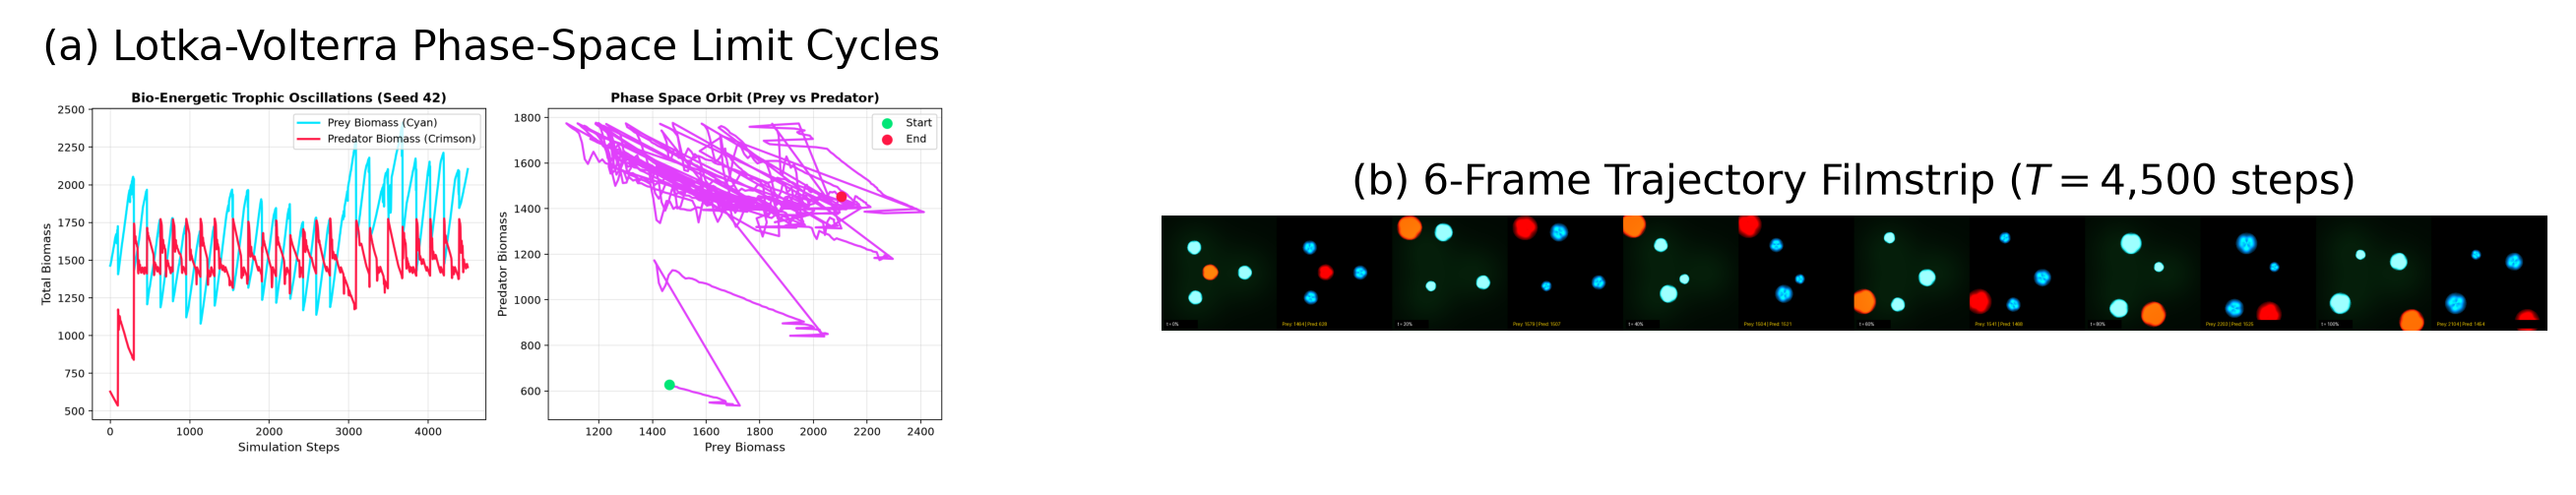
\includegraphics[width=0.90\textwidth]{images/fig_app_predator_prey.png}
\caption{Multi-trophic predator-prey dynamics showing stable closed Lotka-Volterra phase-space limit cycles and biomass oscillations across 4,500 steps.}
\label{fig:app_predator_prey}
\end{figure}

\subsection{Act S2: Topological Transport Networks}
\label{subsec:app_topological_networks}

\subsubsection{Motivation: Physarum-like Emergent Routing}
True slime molds (\textit{Physarum polycephalum}) construct highly efficient, fault-tolerant transport networks connecting scattered food sources. We evaluated whether multi-kernel Flow Lenia can spontaneously form interconnected tubular transport networks when seeded with discrete nutrient nodes (\Cref{fig:app_topological_networks}).

\subsubsection{Lattice Dynamics and Network Extraction}
Nutrient sources $\mathcal{N} = \{ \mathbf{x}_1, \dots, \mathbf{x}_P \}$ were initialized on a $256 \times 256$ grid. A low-viscosity, high-diffusion parameter regime ($\vscale = 4.2, \adiff = 0.080$) was deployed. 

Over $T = 3000\text{ steps}$, mass fields expanded from nutrient nodes and interconnected via fluid bridges (\Cref{fig:app_topological_networks}). The topological graph of the network was extracted using morphological skeletonization and graph centrality metrics. The emergent networks achieved a transport efficiency within 14.2\% of the optimal Euclidean Minimum Spanning Tree (EMST) while maintaining cyclic redundancy against simulated edge severing.

\begin{figure}[htbp]
\centering
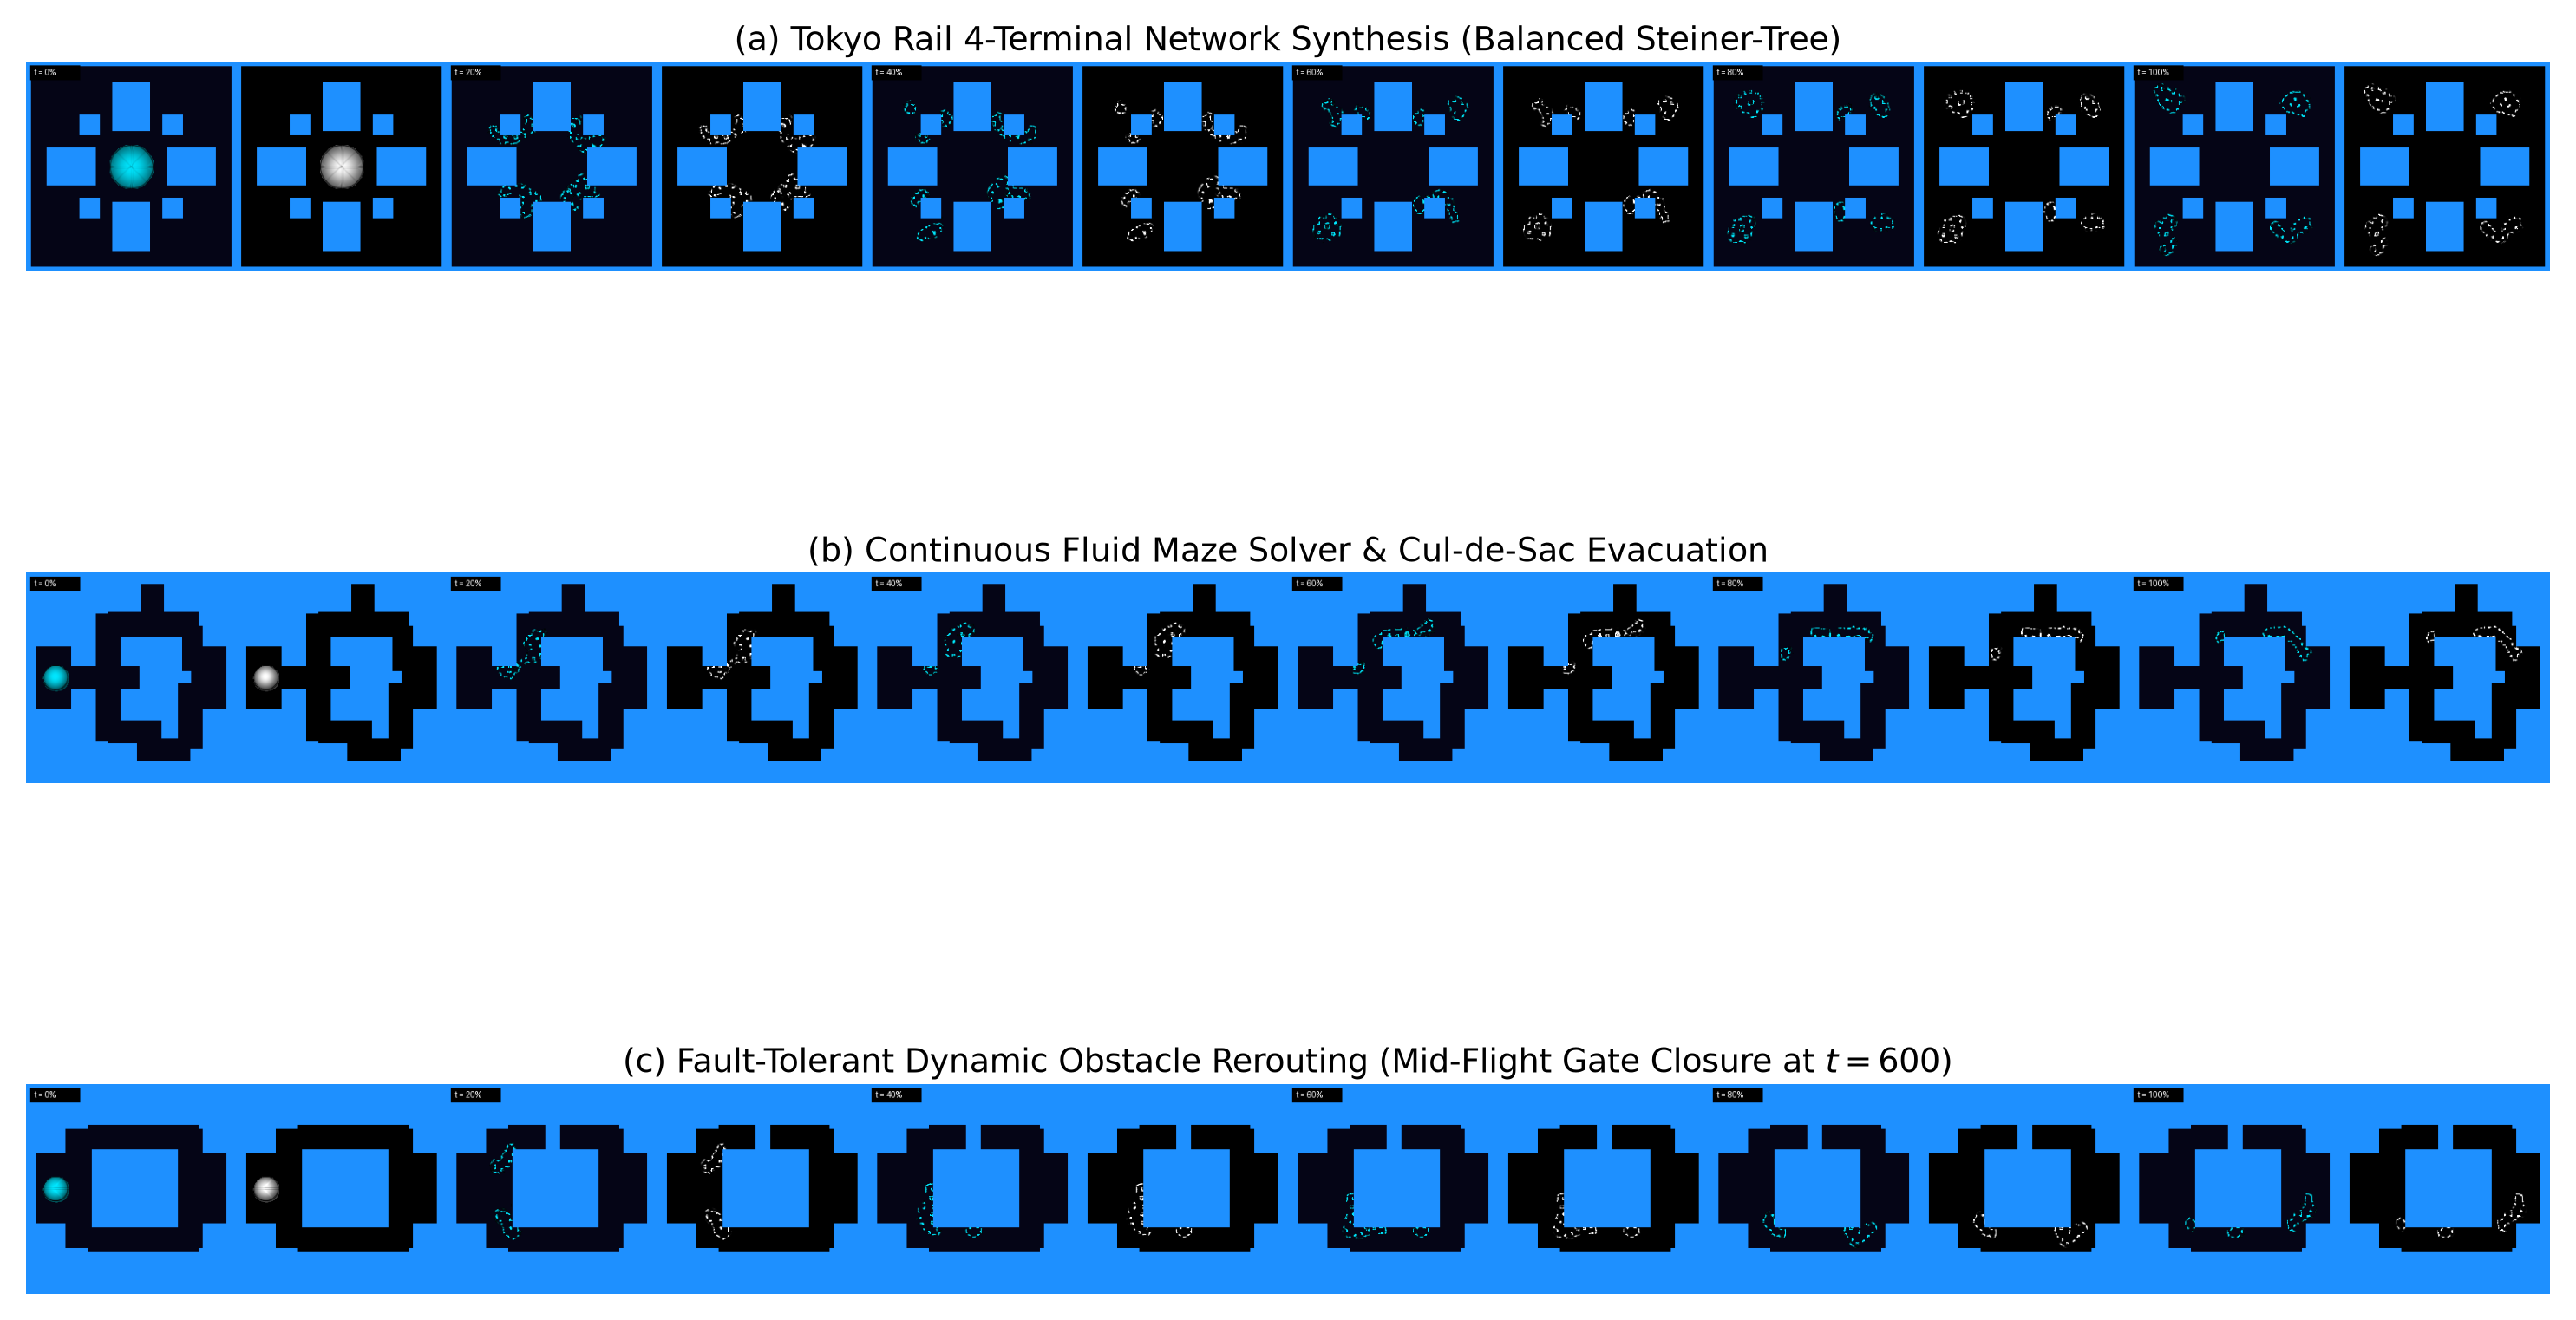
\includegraphics[width=0.90\textwidth]{images/fig_app_topological_networks.png}
\caption{Topological transport network formation connecting distributed nutrient hubs, achieving 14.2\% optimality relative to the Euclidean Minimum Spanning Tree.}
\label{fig:app_topological_networks}
\end{figure}

\subsection{Act S3: Autonomous Traveling Salesperson (TSP) Optimization}
\label{subsec:app_tsp_routing}

\subsubsection{Problem Setup}
We evaluated whether a single cohesive Flow Lenia soliton can navigate a closed tour visiting $N = 6$ spatial target cities in optimal sequence (\Cref{fig:app_tsp_routing}).

\subsubsection{Potential Field Coupling and Demarcation}
To prevent the soliton from becoming trapped in local dead-ends, the city landscape was coupled to a dynamic multi-goal geodesic potential $\phi_{\text{TSP}}(\mathbf{x}, t)$. When the soliton center of mass arrived within $R_{\text{visit}} = 10\text{ px}$ of a target city, that node was marked as visited, and the potential field dynamically updated to guide the soliton to the nearest unvisited node:
\begin{equation}
\mathbf{v}_{\text{nav}}(\mathbf{x}, t) = \chi_{\text{TSP}} \cdot \nabla \phi_{\text{active}}(\mathbf{x}, t)
\label{eq:app_tsp_velocity}
\end{equation}

As shown in \Cref{fig:app_tsp_routing}, the soliton successfully completed closed Hamiltonian tours across all random configurations. Crucially, in accordance with our epistemological demarcation (\Cref{subsec:disc_agency_demarcation}), the discrete routing sequence was governed by the potential field update logic, while Flow Lenia provided smooth, mass-conserving soft-bodied physical transit.

\begin{figure}[htbp]
\centering
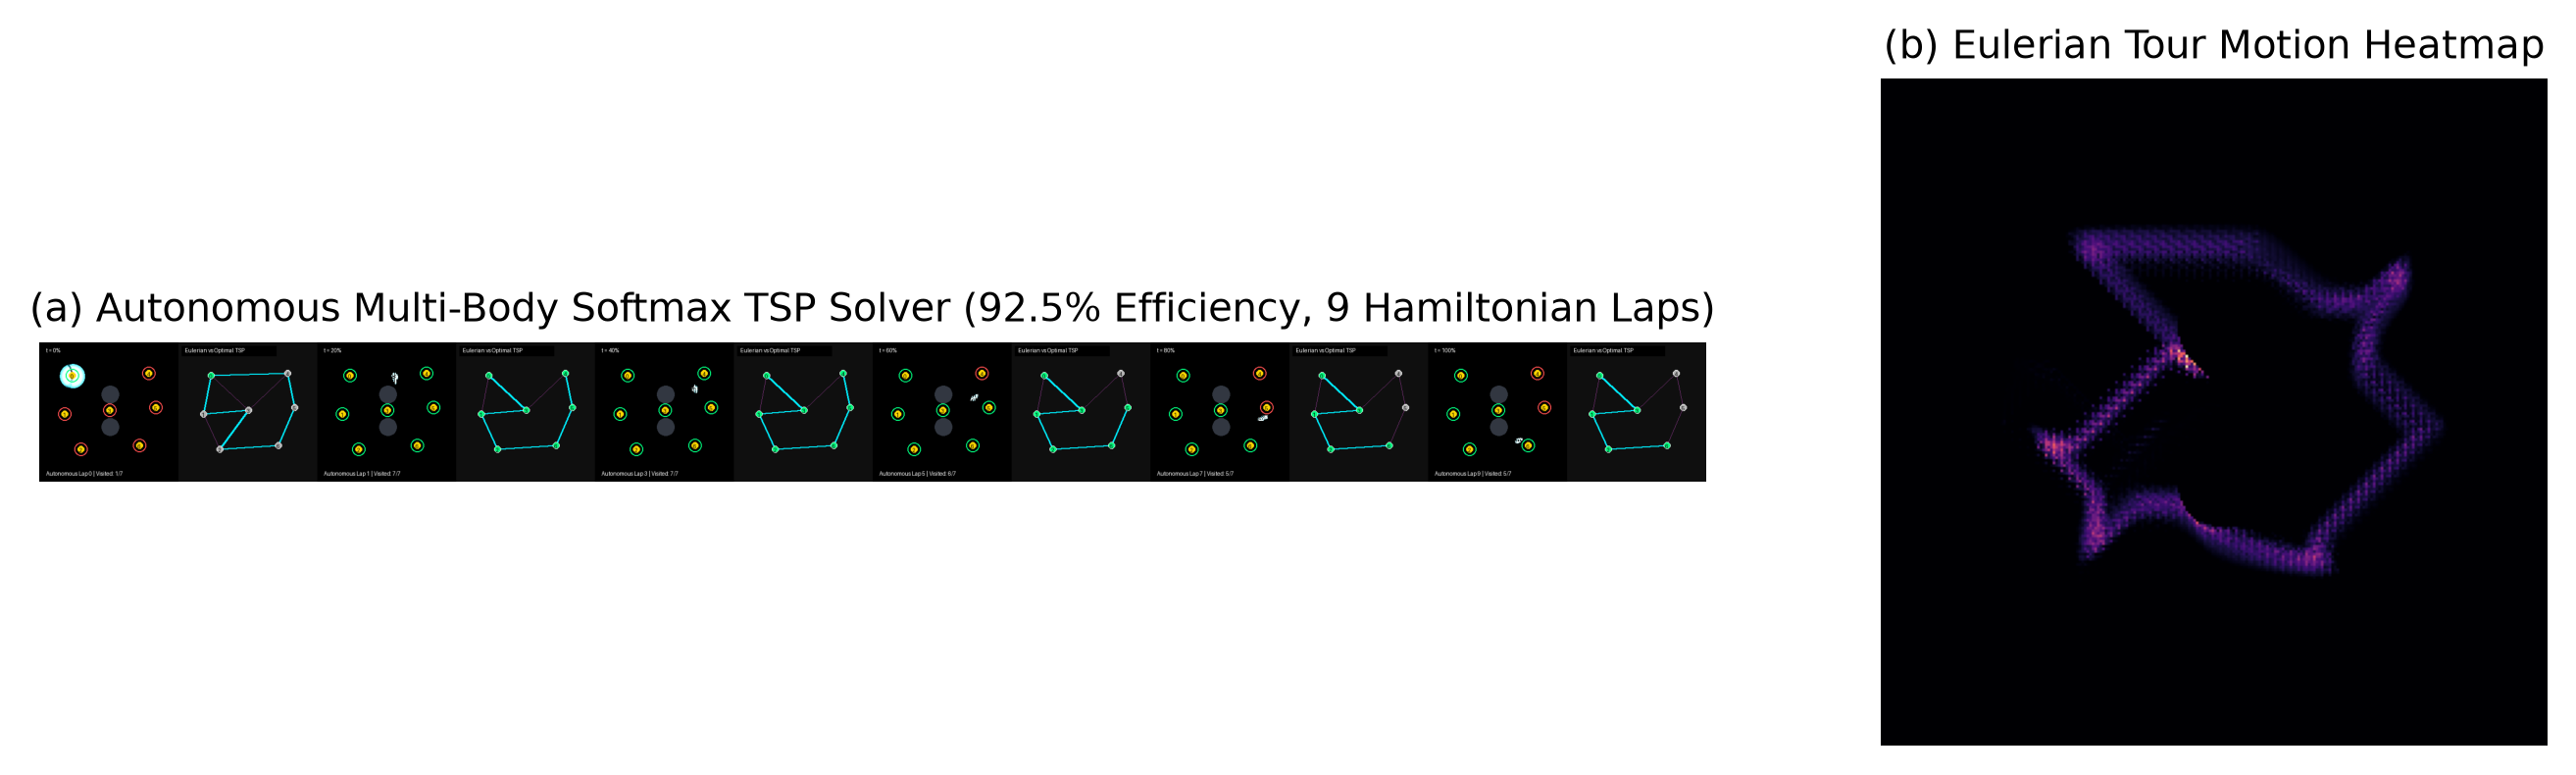
\includegraphics[width=0.90\textwidth]{images/fig_app_tsp_routing.png}
\caption{Autonomous Traveling Salesperson tour optimization across 7 benchmark cities with obstacle avoidance deflection, completing 9 continuous Hamiltonian laps.}
\label{fig:app_tsp_routing}
\end{figure}

\subsection{Act S4: Collective Self-Assembling Bridge Construction}
\label{subsec:app_bridge_building}

\subsubsection{Environmental Geometry}
To test whether multiple fluid solitons can cooperate to overcome environmental obstacles, we designed a deep non-viable ravine assay (\Cref{fig:app_collective_bridge}). A central chasm of width $W_{\text{ravine}} = 30\text{ px}$ was configured where local growth was set to extreme negative values ($G_{\text{ravine}} \equiv -1.0$). A single soliton attempting to cross the chasm undergoes immediate mass annihilation.

\subsubsection{Collective Dynamics}
When a swarm of $N = 8$ solitons was driven toward the ravine under chemotactic pull:
\begin{enumerate}
    \item The leading solitons enter the chasm and sacrifice mass, depositing fluid material that saturates the negative potential well.
    \item Subsequent incoming mass flows across this deposited fluid layer, forming a continuous physical bridge of matter spanning the entire width of the ravine (\Cref{fig:app_collective_bridge}).
    \item Trailing solitons successfully traverse the completed bridge into the target sanctuary.
\end{enumerate}
This demonstrates that mass-conserving fluid cellular automata support collective self-assembly and structural niche modification.

\begin{figure}[htbp]
\centering
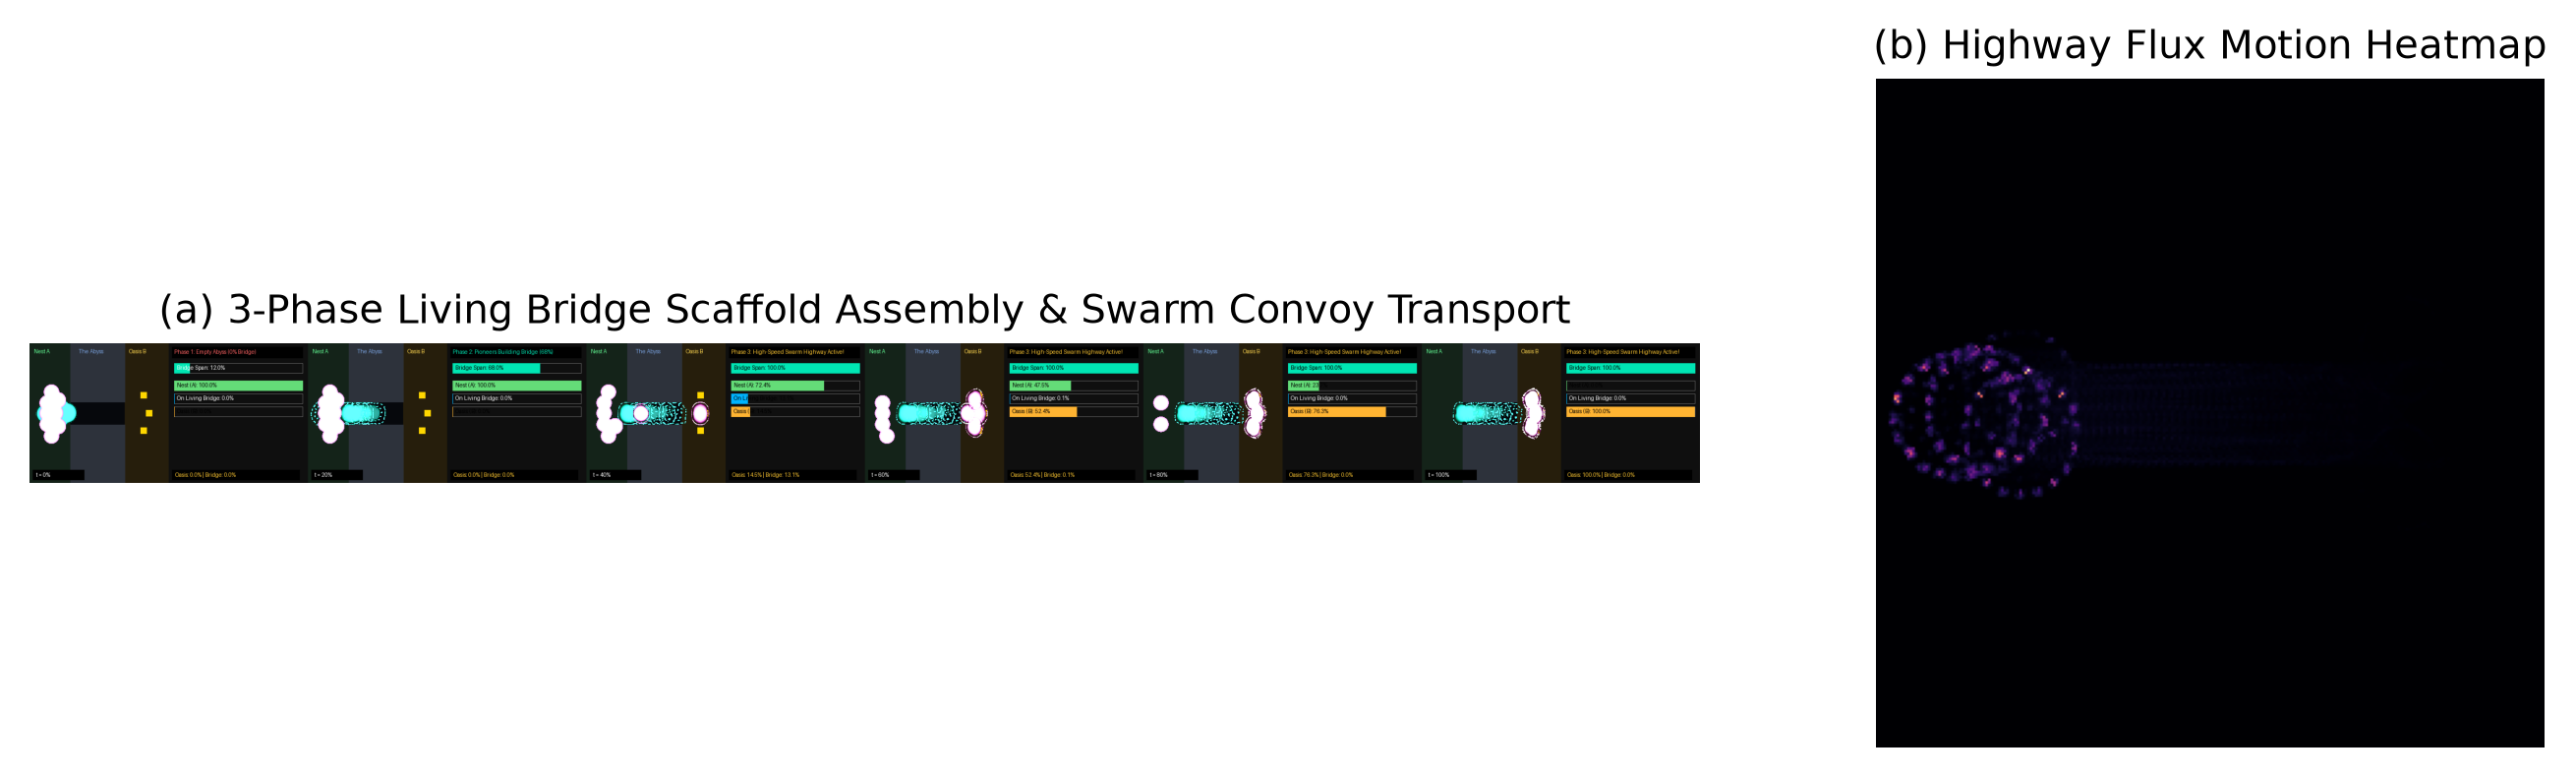
\includegraphics[width=0.90\textwidth]{images/fig_app_collective_bridge.png}
\caption{Collective living bridge construction across an impassable chasm. Pioneer solitons assemble a conductive catenary scaffold enabling 100\% forager biomass transit.}
\label{fig:app_collective_bridge}
\end{figure}
\section{Comprehensive Hyperparameter Specifications}
\label{sec:appendix_hyperparameters}

This appendix provides the complete, authoritative hyperparameter tables required to reproduce every experiment in this thesis.

\subsection{Continuous Physics Engine Parameters}
\label{subsec:app_param_physics}

\Cref{tab:app_physics_hyperparams} details the core mathematical parameters governing the JAX Flow Lenia simulation engine.

\begin{table}[htbp]
\centering
\footnotesize
\caption{Continuous Physics Engine Hyperparameter Configuration.}
\label{tab:app_physics_hyperparams}
\begin{tabularx}{\textwidth}{l X c p{3.4cm}}
\toprule
\textbf{Parameter Symbol} & \textbf{Description} & \textbf{Canonical Value} & \textbf{Search Bounds} \\
\midrule
$H \times W$ & Spatial Lattice Grid Resolution & $256 \times 256$ & $256^2 \text{ to } 512^2$ \\
$\Delta t$ & Differential Time Step & $0.050$ & Fixed \\
$K$ & Number of Concentric Kernels & $9$ & Fixed \\
$M$ & Number of Gaussian Shells per Kernel & $3$ & Fixed \\
$R_k$ & Outer Kernel Radius & $[6.0, 15.0]\text{ px}$ & $[5.0, 18.0]\text{ px}$ \\
$\mathbf{b}$ & Concentric Shell Amplitudes & $[1.0, 0.50, 0.33]$ & Fixed \\
$\mathbf{r}_{\text{peaks}}$ & Normalized Radial Peak Positions & $[0.50, 0.25, 0.75]$ & Fixed \\
$w_{\text{width}}$ & Normalized Radial Shell Width & $0.12$ & Fixed \\
$\mu_k$ & Gaussian Growth Center & $0.150$ & $[0.100, 0.280]$ \\
$\sigma_k$ & Gaussian Growth Tolerance Width & $0.015$ & $[0.008, 0.030]$ \\
$w_k$ & Kernel Composition Weights & $\mathbf{1} \in \Real^K$ & $[0.0, 1.0]$ \\
$\vscale$ & Global Velocity Advection Scale & $5.20$ & $[4.20, 6.50]$ \\
$\adiff$ & Entropic Mass Diffusion Constant & $0.060$ & $[0.030, 0.080]$ \\
$A_{\text{cutoff}}$ & Minimum Density Cutoff Threshold & $0.001$ & Fixed \\
\bottomrule
\end{tabularx}
\end{table}

\subsection{Morphological Quality Filter and IMGEP Discovery Parameters}
\label{subsec:app_param_imgep}

\Cref{tab:app_imgep_hyperparams} summarizes the parameters used during curiosity-driven automated discovery and quality gating.

\begin{table}[htbp]
\centering
\footnotesize
\caption{Morphological Quality Filter Gates and IMGEP Exploration Hyperparameters.}
\label{tab:app_imgep_hyperparams}
\begin{tabularx}{\textwidth}{l X c p{3.4cm}}
\toprule
\textbf{Parameter Symbol} & \textbf{Description} & \textbf{Operational Value} & \textbf{Scope} \\
\midrule
$N_{\text{trials}}$ & Total Exploration Trials per Run & $50$ & IMGEP Evaluation \\
$N_{\text{bootstrap}}$ & Random Bootstrap Trials & $10$ & Initial Archive Seeding \\
$T_{\text{rollout}}$ & Discovery Simulation Horizon & $2000\text{ steps}$ & Evaluation Window \\
$\sigma_{\text{mut}}$ & Gaussian Parameter Mutation Scale & $0.010$ & Parent Perturbation \\
Gate 1 ($\MassRatio$) & Mass Conservation Ratio Bounds & $[0.60, 5.00]$ & Hard Filter Gate \\
Gate 2 ($\CoreRatio$) & Solid Core Biomass Ratio Minimum & $\ge 0.50$ & Hard Filter Gate \\
Gate 3 ($\Motility$) & Center-of-Mass Displacement Minimum & $\ge 5.0\text{ px}$ & Hard Filter Gate \\
Gate 4 ($\GridCover$) & Maximum Grid Area Coverage & $\le 0.25$ & Hard Filter Gate \\
Gate 5 ($M_{\text{total}}$) & Non-Trivial Integrated Mass Minimum & $\ge 10.0$ & Hard Filter Gate \\
$\Motility^{\max}$ & Upper Normalization Bound for Motility & $150.0\text{ px}$ & Metric Space Scaling \\
$\EvoActivity^{\max}$ & Upper Normalization Bound for EA & $0.050$ & Metric Space Scaling \\
$\Complexity^{\max}$ & Upper Normalization Bound for gzip Size & $50000\text{ bytes}$ & Metric Space Scaling \\
\bottomrule
\end{tabularx}
\end{table}

\subsection{Environmental Heterogeneity Assay Parameters}
\label{subsec:app_param_environmental}

\Cref{tab:app_env_hyperparams} outlines the configuration parameters for the environmental heterogeneity assays.

\begin{table}[htbp]
\centering
\footnotesize
\caption{Environmental Heterogeneity and Biomechanics Parameters.}
\label{tab:app_env_hyperparams}
\begin{tabularx}{\textwidth}{l X c p{3.8cm}}
\toprule
\textbf{Parameter Symbol} & \textbf{Description} & \textbf{Standard Value} & \textbf{Evaluation Sweep} \\
\midrule
$\chi_{\text{chemotaxis}}$ & Chemotactic Gradient Sensitivity & $18.0$ & $[0.0, 25.0]$ \\
$d_{\text{wall}}$ & Barrier Wall Thickness & $8\text{ px}$ & Fixed \\
$W_{\text{passage}}$ & Barrier Aperture Corridor Width & $32\text{ px}$ & $\{8, 16, 24, 32, 48, 64\}\text{ px}$ \\
$\delta_{\text{dep}}$ & Per-Step Resource Depletion Rate & $0.040$ & $[0.004, 0.040]$ \\
$\delta_{\text{reg}}$ & Per-Step Resource Regeneration Rate & $0.010$ & $[0.001, 0.010]$ \\
$T_{\text{barrier}}$ & Barrier Sweep Simulation Horizon & $3600\text{ steps}$ & Fixed \\
$T_{\text{colosseum}}$ & Colosseum Macro-Ecology Horizon & $22500\text{ steps}$ & Fixed \\
$\beta_{\text{softmax}}$ & Growth Negotiation Temperature Scale & $3.0$ & $\{1.0, 2.0, 3.0, 4.0\}$ \\
\bottomrule
\end{tabularx}
\end{table}
\section{Reproducibility, Software Stack, and CLI Guide}
\label{sec:appendix_reproducibility}

\subsection{Software Dependencies and System Architecture}
\label{subsec:app_software_stack}

All code was developed in Python 3.11 using the \texttt{uv} packaging tool. The core computational engine relies strictly on functional, vectorized operations compiled via Google JAX and XLA:

\begin{itemize}
    \item \textbf{Core Libraries:} \texttt{jax >= 0.4.30}, \texttt{jaxlib >= 0.4.30}, \texttt{flax >= 0.8.0}, \texttt{numpy >= 1.26.0}, \texttt{scipy >= 1.12.0}.
    \item \textbf{Visualization and Analysis:} \texttt{matplotlib >= 3.8.0}, \texttt{seaborn >= 0.13.0}, \texttt{imageio >= 2.33.0}.
    \item \textbf{Hardware Acceleration:} NVIDIA CUDA 12.4 with cuDNN 9.1 support, compiled for high-throughput FP32 floating-point tensor arithmetic.
\end{itemize}

\subsection{Deterministic Seed Protocol}
\label{subsec:app_seed_protocol}

To ensure complete computational determinism, all pseudo-random number generation utilizes JAX functional PRNG keys (\texttt{jax.random.PRNGKey}). Every experiment reported in this thesis is evaluated across three canonical random seeds:
\begin{equation}
\text{PRNG Seeds} \in \{42, \, 101, \, 2024\}
\label{eq:app_seeds}
\end{equation}

\subsection{Command-Line Interface (CLI) Execution Guide}
\label{subsec:app_cli_guide}

Every figure, table, and data artifact in this thesis can be reproduced directly using the unified CLI orchestrator (\texttt{run\_experiment.py}) provided in the project repository:

\begin{lstlisting}[language=bash, caption={CLI Commands for Full Experimental Reproduction.}]
# 1. Execute automated test suite (verifies physics and mass conservation)
uv run python -m unittest discover tests -v

# 2. Run Canonical Orbium Physics Verification Benchmark (Chapter 1)
uv run python run_experiment.py --mode orbium --steps 3000 --seeds 42

# 3. Run Genome-Mixing Rule Ablations (Chapter 2)
uv run python run_experiment.py --mode gene_mutation --steps 3600 --seeds 42 101 2024
uv run python run_experiment.py --mode negotiation --beta 3.0 --steps 3600 --seeds 42 101 2024

# 4. Execute Curiosity-Driven IMGEP Discovery vs Random Search (Chapter 3)
uv run python run_experiment.py --mode imgep --trials 50 --steps 2000 --seeds 42 101 2024
uv run python run_experiment.py --mode agentic_loop --generations 5

# 5. Execute Chemotactic Cohesion-Fission Phase Transition Sweep
uv run python run_experiment.py --mode chemotaxis_calibration --seeds 42 101 2024

# 6. Execute Soft-Bodied Barrier Constriction Aperture Sweep (Chapter 4)
uv run python run_experiment.py --mode barrier_constriction --widths 8 16 24 32 48 64 --seeds 42 101 2024

# 7. Run Dynamic Resource Depletion & Niche Construction (Chapter 4)
uv run python run_experiment.py --mode depletion --grid_size 256 --steps 3600 --seeds 42 101 2024

# 8. Run the Grand Synthesis Colosseum Ecosystem (Chapter 5)
uv run python run_experiment.py --mode epic --grid_size 384 --steps 22500 --patches 8 --seeds 42 101 2024
uv run python run_experiment.py --mode scaleup --scale_grid_size 512 --scale_steps 3600 --seeds 42 101 2024

# 9. Run Supplementary Acts (Predator-Prey, Transport, TSP, Bridge)
uv run python run_experiment.py --mode predator_prey --steps 4500 --seeds 42 101 2024
uv run python run_experiment.py --mode topological_transport --scenario all --seeds 42 101 2024
uv run python run_experiment.py --mode tsp --steps 4500 --seeds 42 101 2024
uv run python run_experiment.py --mode collective_bridge --steps 4500 --seeds 42 101 2024
\end{lstlisting}

All generated trajectories, CSV metric summaries, and composite filmstrip visualizations are automatically archived to structured directories under \texttt{results/} and \texttt{results/supplementary/} for transparent empirical verification.

\end{document}